%%%%%%%%%%%%%%%%%%%%%%%%
%
% $Autor: Wings $
% $Datum: 2019-07-09 09:26:07Z $
% $Pfad: Vorlesungen/WS_19_20/Projekte/KandaNeuralnetwork/latex - Ausarbeitung/Kapitel/Hardware.tex $
% $Version: 4440 $
%
%%%%%%%%%%%%%%%%%%%%%%%%


%todo GitLab\ToDo\TinyML
% TinyML Seite 222

\section{Arduino Nano 33 BLE Sense}



\url{https://www.reichelt.de/de/de/arduino-nano-33-ble-sense-nrf52840-ohne-header-ard-nano-33bles-p261306.html?PROVID=2788&gclid=Cj0KCQjwna2FBhDPARIsACAEc_Uui0sowk2McNvt69o9wzQJtqHWW2n5l_OHng2pSRcmfYqUsiosbdUaAp47EALw_wcB&&r=1}

\subsection{ARD NANO 33BLE S}

Arduino Nano BLE Sense - klein, stromsparend und mit Bluetooth, basierend auf dem  Microcontroller nRF52480.

Dieses kompakte und zuverlässige Nano-Board enthält das Modul NINA B306 für BLE- und Bluetooth 5-Kommunikation. Das Modul basiert auf dem nordischen Prozessor nRF 52840, der einen leistungsstarken Cortex M4F enthält. Es verfügt über einen großen Satz an Sensoren, die die Erstellung innovativer und interaktiver Designs ermöglichen.

Seine Architektur, die vollständig mit Arduino IDE Online und Offline kompatibel ist, verfügt über eine 9-achsige Trägheitsmesseinheit (IMU) mit Temperatur-, Druck-, Feuchtigkeits-, Licht-, Farb- und sogar Gestensensoren sowie über ein Mikrofon, das über die spezialisierten Bibliotheken verwaltet wird. Der im Vergleich zu anderen Boards gleicher Größe geringere Stromverbrauch und der Nano-Formfaktor eröffnen ein breites Anwendungsspektrum.

Dies ermöglicht die Entwicklung von tragbaren Geräten und gestenbasierten Projekten, die mit anderen Geräten aus nächster Nähe kommunizieren müssen.

Der Arduino Nano 33 BLE Sense ist dank des Multiprotokolls BT 5.0 Radio ideal für interaktive Automatisierungsprojekte.

Hinweis: Dieses Board wird ohne integriertem Header geliefert.



\url{https://store.arduino.cc/arduino-nano-33-ble-sense}


\begin{figure}[!h]
  \centering
  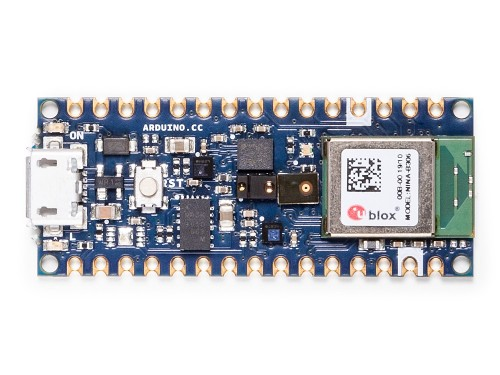
\includegraphics[width=50mm]{Arduino/ArduinoNano33BLESense}
  
  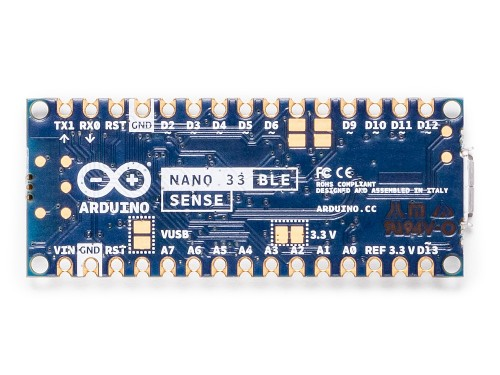
\includegraphics[width=50mm]{Arduino/ArduinoNano33BLESense2}
  
  \caption{Arduino Nano 33 BLE Sense \href{https://store.arduino.cc/arduino-nano-33-ble-sense}{Arduino Store}}
\end{figure}


\section{Tutorial}



\subsection{Was wir bauen}

Wir werden eine eingebettete Anwendung erstellen, die ein Modell zur Klassifizierung von Bildern verwendet, die von einer Kamera aufgenommen wurden. Das Modell wird so trainiert, dass es erkennt, wenn eine Person in der Kameraeingabe vorhanden ist. Das bedeutet, dass unsere Anwendung in der Lage sein wird, die An- oder Abwesenheit einer Person zu erkennen und eine entsprechende Ausgabe zu erzeugen.

Dies ist im Wesentlichen der intelligente Vision-Sensor, den wir etwas früher beschrieben haben. Wenn eine Person erkannt wird, lässt unser Beispielcode eine LED aufleuchten - aber Sie können ihn erweitern, um alle möglichen Projekte zu steuern.

\url{https://github.com/tensorflow/tensorflow/tree/master/tensorflow/lite/micro/examples/person_detection}


\subsection{Bemerkung}

TensorFlow Lite fügt regelmäßig Unterstützung für neue Geräte hinzu. Wenn also das Gerät, das Sie verwenden möchten, hier nicht aufgeführt ist, lohnt es sich, in der \FILE{README.md} des Beispiels nachzusehen. Sie können dort auch nach aktualisierten Deployment-Anweisungen suchen, wenn Sie bei der Ausführung dieser Schritte auf Probleme stoßen.


Anders als bei den vorherigen Kapiteln benötigen Sie für diese Anwendung zusätzliche Hardware. Da keines der beiden Boards eine integrierte Kamera hat, empfehlen wir den Kauf eines Kameramoduls. Diese Informationen finden Sie im Abschnitt über das jeweilige Gerät.

\subsection{Kamera-Module}

Kameramodule sind elektronische Bauteile auf Basis von Bildsensoren, die Bilddaten digital erfassen. Der Bildsensor wird mit einem Objektiv und einer Steuerelektronik kombiniert und das Modul wird in einer Form hergestellt, die einfach an ein Elektronikprojekt angebracht werden kann.

Lassen Sie uns zunächst die Struktur unserer Anwendung durchgehen. Es ist viel einfacher, als Sie vielleicht erwarten.


\subsection{Anwendungsarchitektur}

Inzwischen haben wir festgestellt, dass eingebettete Anwendungen für maschinelles Lernen die folgende Abfolge von Dingen tun:

\begin{itemize}
  \item Erhalten Sie eine Eingabe.
  \item Verarbeiten Sie die Eingabe vor, um Merkmale zu extrahieren, die für die Eingabe in ein Modell geeignet sind.
  \item Ausführen der Inferenz auf die verarbeitete Eingabe.
  \item Die Ausgabe des Modells nachverarbeiten, um sie sinnvoll zu nutzen.
  \item Verwenden Sie die resultierenden Informationen, um etwas zu bewirken.
\end{itemize}

In Kapitel 7 haben wir gesehen, wie dies auf die Wake-Word-Erkennung angewendet wird, die Audio als Eingabe verwendet. Dieses Mal werden wir als Eingabe Bilddaten verwenden. Das hört sich vielleicht komplizierter an, ist aber in Wirklichkeit viel einfacher zu handhaben als Audio.

Bilddaten werden üblicherweise als ein Array von Pixelwerten dargestellt. Wir werden unsere Bilddaten von eingebetteten Kameramodulen beziehen, die alle Daten in diesem Format bereitstellen. Unser Modell erwartet auch, dass seine Eingabe ein Array von Pixelwerten ist. Aus diesem Grund müssen wir nicht viel Vorarbeit leisten, bevor wir die Daten in unser Modell einspeisen.

Angesichts der Tatsache, dass wir nicht viel Vorverarbeitung machen müssen, wird unsere Anwendung ziemlich einfach sein. Sie nimmt einen Schnappschuss der Daten von einer Kamera auf, speist ihn in ein Modell ein und bestimmt, welche Ausgabeklasse erkannt wurde. Anschließend zeigt sie das Ergebnis auf einfache Weise an.

Bevor wir weitermachen, wollen wir ein wenig mehr über das Modell erfahren, das wir verwenden werden.

\subsection{Einführung in unser Modell}

In Kapitel 7 haben wir gelernt, dass faltungsneuronale Netze neuronale Netze sind, die für die Arbeit mit mehrdimensionalen Tensoren ausgelegt sind, bei denen die Informationen in den Beziehungen zwischen Gruppen benachbarter Werte enthalten sind. Sie sind besonders gut für die Arbeit mit Bilddaten geeignet.

Unser Personenerkennungsmodell ist ein neuronales Faltungsnetzwerk, das auf dem Visual Wake Words-Datensatz trainiert wurde. Dieser Datensatz besteht aus 115.000 Bildern, von denen jedes mit der Angabe versehen ist, ob es eine Person enthält oder nicht.

Das Modell ist 250 KB groß und damit deutlich größer als unser Sprachmodell. Diese zusätzliche Größe belegt nicht nur mehr Speicher, sondern bedeutet auch, dass es viel länger dauert, eine einzelne Inferenz auszuführen.

Das Modell akzeptiert 96 × 96-Pixel-Graustufenbilder als Eingabe. Jedes Bild wird als 3D-Tensor mit der Form (96, 96, 1) bereitgestellt, wobei die letzte Dimension einen 8-Bit-Wert enthält, der ein einzelnes Pixel repräsentiert. Der Wert gibt den Farbton des Pixels an, der von 0 (vollständig schwarz) bis 255 (vollständig weiß) reicht.

Unsere Kameramodule können Bilder in verschiedenen Auflösungen zurückgeben, daher müssen wir sicherstellen, dass sie auf 96 × 96 Pixel verkleinert werden. Außerdem müssen wir vollfarbige Bilder in Graustufen umwandeln, damit sie mit dem Modell funktionieren.

\url{https://arxiv.org/abs/1906.05721}


Sie denken vielleicht, dass 96 × 96 Pixel eine winzige Auflösung ist, aber sie ist mehr als ausreichend, um eine Person in jedem Bild zu erkennen. Modelle, die mit Bildern arbeiten, akzeptieren oft erstaunlich kleine Auflösungen. Eine Erhöhung der Eingabegröße eines Modells führt zu abnehmenden Erträgen, und die Komplexität des Netzwerks steigt stark an, wenn die Größe der Eingabe skaliert. Aus diesem Grund arbeiten selbst moderne Bildklassifizierungsmodelle in der Regel mit einer maximalen Auflösung von 320 × 320 Pixeln.

Das Modell gibt zwei Wahrscheinlichkeiten aus: eine, die die Wahrscheinlichkeit angibt, dass eine Person in der Eingabe vorhanden war, und eine andere, die die Wahrscheinlichkeit angibt, dass niemand dort war. Die Wahrscheinlichkeiten reichen von 0 bis 255.

Unser Personenerkennungsmodell verwendet die MobileNet-Architektur, eine bekannte und erprobte Architektur, die für die Bildklassifizierung auf Geräten wie Mobiltelefonen entwickelt wurde. In Kapitel 10 werden Sie erfahren, wie dieses Modell an Mikrocontroller angepasst wurde und wie Sie Ihr eigenes Modell trainieren können. Lassen Sie uns nun weiter erkunden, wie unsere Anwendung funktioniert.


\subsection{Alle beweglichen Teile}


Figure~\ref{tflite:Ablauf} shows the structure of our person detection application.

\begin{figure}
  \centering
  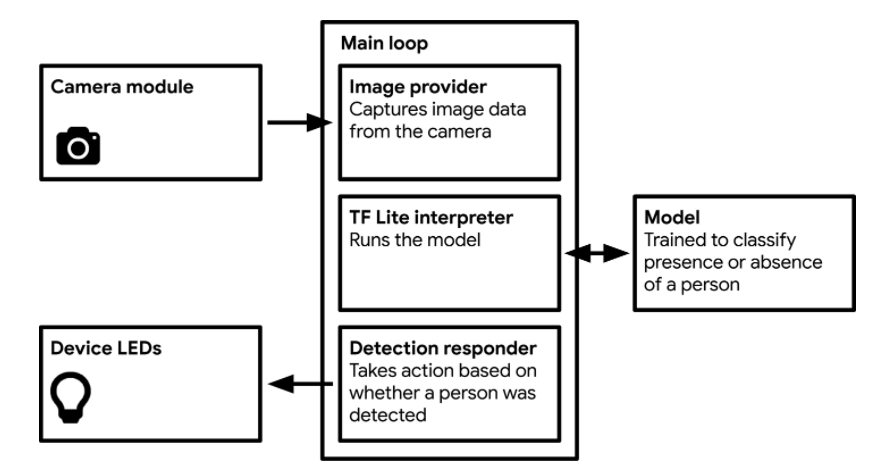
\includegraphics[width=0.9\textwidth]{Arduino/tfLiteAblauf}
  \caption{Diagram of the components of our person detection application}\label{tflite:Ablauf}
\end{figure}

Wie wir bereits erwähnt haben, ist dies viel einfacher als die Wake-Word-Anwendung, da wir die Bilddaten direkt in das Modell übergeben können - es ist keine Vorverarbeitung erforderlich.

Ein weiterer Aspekt, der die Dinge einfach hält, ist, dass wir die Ausgabe des Modells nicht mitteln. Unser Wake-Word-Modell wurde mehrmals pro Sekunde ausgeführt, so dass wir seine Ausgabe mitteln mussten, um ein stabiles Ergebnis zu erhalten. Unser Personenerkennungsmodell ist viel größer und braucht viel länger, um die Inferenz auszuführen. Das bedeutet, dass es keine Notwendigkeit gibt, seine Ausgabe zu mitteln.

Der Code besteht aus fünf Hauptteilen:

\textbf{Main loop}

Wie die anderen Beispiele läuft auch unsere Anwendung in einer Endlosschleife. Da unser Modell jedoch viel größer und komplexer ist, dauert es länger, bis die Inferenz ausgeführt wird. Je nach Gerät können wir eine Inferenz alle paar Sekunden erwarten, anstatt mehrere Inferenzen pro Sekunde.

\textbf{Image provider}

Diese Komponente erfasst Bilddaten von der Kamera und schreibt sie in den Eingangstensor. Die Methoden zur Erfassung von Bildern variieren von Gerät zu Gerät, daher kann diese Komponente überschrieben und angepasst werden.

\textbf{TensorFlow Lite interpreter}

Der Interpreter führt das TensorFlow Lite Modell aus und transformiert das Eingabebild in einen Satz von Wahrscheinlichkeiten.

\textbf{Modell}

Das Modell wird als Datenarray eingebunden und vom Interpreter ausgeführt. Mit 250 KB ist dieses Modell unangemessen groß, um es an das TensorFlow GitHub Repository zu übergeben. Aus diesem Grund wird es vom Makefile heruntergeladen, wenn das Projekt gebaut wird. Wenn Sie einen Blick darauf werfen wollen, können Sie es selbst unter \FILE{tf\_lite\_micro\_person\_data\_grayscale.zip} herunterladen.

\textbf{Detection responder}


Der Erkennungsresponder nimmt die vom Modell ausgegebenen Wahrscheinlichkeiten und verwendet die Ausgabefähigkeiten des Geräts, um sie anzuzeigen. Wir können ihn für verschiedene Gerätetypen überschreiben. In unserem Beispielcode leuchtet eine LED auf, aber Sie können ihn so erweitern, dass er so ziemlich alles tun kann.

Um ein Gefühl dafür zu bekommen, wie diese Teile zusammenpassen, werfen wir einen Blick auf ihre Tests.

\textbf{Durch die Tests gehen}

Diese Anwendung ist schön einfach, da es nur ein paar Tests zu durchlaufen gibt. Sie können sie alle im GitHub-Repository finden:

\FILE{person\_detection\_test.cc}

Zeigt, wie eine Inferenz auf ein Array, das ein einzelnes Bild repräsentiert, ausgeführt werden kann

\FILE{image\_provider\_test.cc}


Zeigt, wie Sie den Bildanbieter verwenden, um ein Bild aufzunehmen

\FILE{detection\_responder\_test.cc}

Zeigt, wie der Erkennungsresponder verwendet wird, um die Ergebnisse der Erkennung auszugeben.

Beginnen wir mit der Untersuchung von \FILE{person\_detection\_test.cc}, um zu sehen, wie die Inferenz auf Bilddaten ausgeführt wird. Da dies das dritte Beispiel ist, das wir durchlaufen haben, sollte Ihnen dieser Code ziemlich vertraut vorkommen. Sie sind auf dem besten Weg, ein eingebetteter ML-Entwickler zu werden!

\textbf{Der Grundablauf}

Beginnen wir mit der Datei \FILE{Person\_detection\_test.cc}. Wir beginnen damit, dass wir die Ops hineinziehen, die unser Modell benötigen wird:

\begin{code}
    

%\lstinputlisting[firstline=1,lastline=136,firstnumber=10,language=c++]{../Code/Nano33BLESense/person_detection/person_detection_test.cc}    

  \begin{lstlisting}
namespace tflite {
    namespace ops {
        namespace micro {
            TfLiteRegistration* Register_DEPTHWISE_CONV_2D();
            TfLiteRegistration* Register_CONV_2D();
            TfLiteRegistration* Register_AVERAGE_POOL_2D();
        }  // namespace micro
    }  // namespace ops
}  // namespace tflite
  \end{lstlisting}
\end{code}


Als nächstes definieren wir eine Tensor-Arena, die für das Modell angemessen groß ist. Wie üblich wurde diese Zahl durch Versuch und Irrtum ermittelt:


\begin{code}
    \begin{lstlisting}
const int tensor_arena_size = 70 * 1024;
uint8_t tensor_arena[tensor_arena_size];
  \end{lstlisting}
\end{code}

Anschließend führen wir die typischen Einrichtungsarbeiten durch, um den Interpreter einsatzbereit zu machen, wozu auch die Registrierung der erforderlichen Ops mit dem \PYTHON{MicroMutableOpResolver} gehört:

\begin{code}
    \begin{lstlisting}
// Set up logging.
tflite::MicroErrorReporter micro_error_reporter;
tflite::ErrorReporter* error_reporter = &micro_error_reporter;

// Map the model into a usable data structure. This doesn't involve any
// copying or parsing, it's a very lightweight operation.
const tflite::Model* model = ::tflite::GetModel(g_person_detect_model_data);
if (model->version() != TFLITE_SCHEMA_VERSION) {
    error_reporter->Report(
    "Model provided is schema version %d not equal "
    "to supported version %d.\n",
    model->version(), TFLITE_SCHEMA_VERSION);
}

// Pull in only the operation implementations we need.
tflite::MicroMutableOpResolver micro_mutable_op_resolver;
micro_mutable_op_resolver.AddBuiltin(
tflite::BuiltinOperator_DEPTHWISE_CONV_2D,
tflite::ops::micro::Register_DEPTHWISE_CONV_2D());
micro_mutable_op_resolver.AddBuiltin(tflite::BuiltinOperator_CONV_2D,
tflite::ops::micro::Register_CONV_2D());
micro_mutable_op_resolver.AddBuiltin(
tflite::BuiltinOperator_AVERAGE_POOL_2D,
tflite::ops::micro::Register_AVERAGE_POOL_2D());

// Build an interpreter to run the model with.
tflite::MicroInterpreter interpreter(model, micro_mutable_op_resolver,
tensor_arena, tensor_arena_size,
error_reporter);
interpreter.AllocateTensors();
  \end{lstlisting}
\end{code}

Unser nächster Schritt ist die Überprüfung des Eingabetensors. Wir prüfen, ob er die erwartete Anzahl von Dimensionen hat und ob seine Dimensionen angemessen dimensioniert sind:

\begin{code}
    \begin{lstlisting}
// Get information about the memory area to use for the model's input.
TfLiteTensor* input = interpreter.input(0);

// Make sure the input has the properties we expect.
TF_LITE_MICRO_EXPECT_NE(nullptr, input);
TF_LITE_MICRO_EXPECT_EQ(4, input->dims->size);
TF_LITE_MICRO_EXPECT_EQ(1, input->dims->data[0]);
TF_LITE_MICRO_EXPECT_EQ(kNumRows, input->dims->data[1]);
TF_LITE_MICRO_EXPECT_EQ(kNumCols, input->dims->data[2]);
TF_LITE_MICRO_EXPECT_EQ(kNumChannels, input->dims->data[3]);
TF_LITE_MICRO_EXPECT_EQ(kTfLiteUInt8, input->type);
  \end{lstlisting}
\end{code}

Daraus können wir erkennen, dass die Eingabe technisch gesehen ein 5D-Tensor ist. Die erste Dimension ist nur ein Wrapper, der ein einzelnes Element enthält. Die folgenden zwei Dimensionen stellen die Zeilen und Spalten der Pixel des Bildes dar. Die letzte Dimension enthält die Anzahl der Farbkanäle, die zur Darstellung jedes Pixels verwendet werden.

Die Konstanten, die die erwarteten Dimensionen angeben, \PYTHON{kNumRows}, \PYTHON{kNumCols} und \PYTHON{kNumChannels}, sind in \FILE{model\_settings.h} definiert. Sie sehen folgendermaßen aus:

\begin{code}
    \begin{lstlisting}
constexpr int kNumCols = 96;
constexpr int kNumRows = 96;
constexpr int kNumChannels = 1;
  \end{lstlisting}
\end{code}

Wie Sie sehen können, wird erwartet, dass das Modell eine Bitmap mit $96 \times 96$ Pixeln akzeptiert. Das Bild wird in Graustufen dargestellt, mit einem Farbkanal für jedes Pixel.

Als nächstes im Code kopieren wir ein Testbild in den Eingangstensor mit einer einfachen for-Schleife:

\begin{code}
    \begin{lstlisting}
// Copy an image with a person into the memory area used for the input.
const uint8_t* person_data = g_person_data;
for (int i = 0; i < input->bytes; ++i) {
    input->data.uint8[i] = person_data[i];
}
  \end{lstlisting}
\end{code}

Die Variable, die die Bilddaten speichert, \PYTHON{g\_person\_data}, wird in der Datei \FILE{person\_image\_data.h} definiert. Um zu vermeiden, dass dem Repository weitere große Dateien hinzugefügt werden, werden die Daten selbst zusammen mit dem Modell heruntergeladen, als Teil von \FILE{tf\_lite\_micro\_person\_data\_grayscale.zip}, wenn die Tests zum ersten Mal ausgeführt werden.

Nachdem wir den Eingabetensor aufgefüllt haben, führen wir die Inferenz durch. Es ist so einfach wie immer:

\begin{code}
    \begin{lstlisting}
// Run the model on this input and make sure it succeeds.
TfLiteStatus invoke_status = interpreter.Invoke();
if (invoke_status != kTfLiteOk) {
    error_reporter->Report("Invoke failed\n");
}
TF_LITE_MICRO_EXPECT_EQ(kTfLiteOk, invoke_status);
  \end{lstlisting}
\end{code}

Wir überprüfen nun den Ausgangstensor, um sicherzustellen, dass er die erwartete Größe und Form hat:

\begin{code}
    \begin{lstlisting}
TfLiteTensor* output = interpreter.output(0);
TF_LITE_MICRO_EXPECT_EQ(4, output->dims->size);
TF_LITE_MICRO_EXPECT_EQ(1, output->dims->data[0]);
TF_LITE_MICRO_EXPECT_EQ(1, output->dims->data[1]);
TF_LITE_MICRO_EXPECT_EQ(1, output->dims->data[2]);
TF_LITE_MICRO_EXPECT_EQ(kCategoryCount, output->dims->data[3]);
TF_LITE_MICRO_EXPECT_EQ(kTfLiteUInt8, output->type);
  \end{lstlisting}
\end{code}

Die Ausgabe des Modells hat vier Dimensionen. Die ersten drei sind nur Umhüllungen für die vierte, die ein Element für jede Kategorie enthält, für die das Modell trainiert wurde.

Die Gesamtzahl der Kategorien ist als Konstante kCategoryCount verfügbar, die sich zusammen mit einigen anderen hilfreichen Werten in \FILE{model\_settings.h} befindet:

\begin{code}
    \begin{lstlisting}
constexpr int kCategoryCount = 3;
constexpr int kPersonIndex = 1;
constexpr int kNotAPersonIndex = 2;
extern const char* kCategoryLabels[kCategoryCount];
  \end{lstlisting}
\end{code}

Wie \PYTHON{kCategoryCount} zeigt, gibt es drei Kategorien in der Ausgabe. Die erste ist zufällig eine unbenutzte Kategorie, die wir ignorieren können. Die Kategorie "Person" kommt an zweiter Stelle, wie wir an ihrem Index erkennen können, der in der Konstante \PYTHON{kPersonIndex} gespeichert ist. An dritter Stelle steht die Kategorie "keine Person", deren Index durch \PYTHON{kNotAPersonIndex} angezeigt wird.

Es gibt auch ein Array von Kategoriebezeichnungen, kCategoryLabels, das in \FILE{model\_settings.cc} implementiert ist:

\begin{code}
    \begin{lstlisting}
const char* kCategoryLabels[kCategoryCount] = {
    "unused",
    "person",
    "notperson",
};
  \end{lstlisting}
\end{code}



\subsection{Extra Dimensions}

Wie \PYTHON{kCategoryCount} zeigt, gibt es drei Kategorien in der Ausgabe. Die erste ist zufällig eine unbenutzte Kategorie, die wir ignorieren können. Die Kategorie "Person" kommt an zweiter Stelle, wie wir an ihrem Index erkennen können, der in der Konstante kPersonIndex gespeichert ist. An dritter Stelle steht die Kategorie "keine Person", deren Index durch kNotAPersonIndex angezeigt wird.

Es gibt auch ein Array von Kategoriebezeichnungen, \PYTHON{kCategoryLabels}, das in \FILE{model\_settings.cc} implementiert ist:
Wie \PYTHON{kCategoryCount} zeigt, gibt es drei Kategorien in der Ausgabe. Die erste ist zufällig eine unbenutzte Kategorie, die wir ignorieren können. Die Kategorie "Person" kommt an zweiter Stelle, wie wir an ihrem Index erkennen können, der in der Konstante \PYTHON{kPersonIndex} gespeichert ist. An dritter Stelle steht die Kategorie "keine Person", deren Index durch \PYTHON{kNotAPersonIndex} angezeigt wird.

Es gibt auch ein Array von Kategoriebezeichnungen, \PYTHON{kCategoryLabels}, das in \FILE{model\_settings.cc} implementiert ist:

\begin{code}
    \begin{lstlisting}
uint8_t person_score = output->data.uint8[kPersonIndex];
uint8_t no_person_score = output->data.uint8[kNotAPersonIndex];
error_reporter->Report(
"person data.  person score: %d, no person score: %d\n", person_score,
no_person_score);
TF_LITE_MICRO_EXPECT_GT(person_score, no_person_score);
  \end{lstlisting}
\end{code}

Da der einzige Dateninhalt des Ausgabetensors die drei \PYTHON{uint8}-Werte sind, die die Klassenwerte darstellen, wobei der erste unbenutzt ist, können wir direkt auf die Werte zugreifen, indem wir \PYTHON{output->data.uint8[kPersonIndex]} und \PYTHON{output->data.uint8[kNotAPersonIndex]} verwenden. Als uint8-Typen haben sie einen Minimalwert von 0 und einen Maximalwert von 255.





\subsection{NOTE}

Wenn die Werte für "Person" und "keine Person" ähnlich sind, kann dies bedeuten, dass das Modell nicht sehr sicher in seiner Vorhersage ist. In diesem Fall können Sie das Ergebnis als nicht schlüssig betrachten.

Als nächstes testen wir auf ein Bild ohne Person, das von \PYTHON{g\_no\_person\_data} gehalten wird:


\begin{code}
    \begin{lstlisting}
const uint8_t* no_person_data = g_no_person_data;
for (int i = 0; i < input->bytes; ++i) {
    input->data.uint8[i] = no_person_data[i];
}
  \end{lstlisting}
\end{code}


Nachdem die Inferenz gelaufen ist, behaupten wir dann, dass der Wert "keine Person" höher ist:

\begin{code}
    \begin{lstlisting}
person_score = output->data.uint8[kPersonIndex];
no_person_score = output->data.uint8[kNotAPersonIndex];
error_reporter->Report(
"no person data.  person score: %d, no person score: %d\n", person_score,
no_person_score);
TF_LITE_MICRO_EXPECT_GT(no_person_score, person_score);
  \end{lstlisting}
\end{code}

Wie Sie sehen können, geht hier nichts Ausgefallenes vor sich. Wir geben zwar Bilder anstelle von Skalaren oder Spektrogrammen ein, aber der Prozess der Inferenz ist ähnlich zu dem, was wir zuvor gesehen haben.

Das Ausführen des Tests ist ähnlich einfach. Geben Sie einfach den folgenden Befehl aus dem Stammverzeichnis des TensorFlow-Repositorys ein:

\begin{code}
    \begin{lstlisting}
make -f tensorflow/lite/micro/tools/make/Makefile \
test_person_detection_test
  \end{lstlisting}
\end{code}

Wenn der Test das erste Mal ausgeführt wird, werden das Modell und die Bilddaten heruntergeladen. Wenn Sie einen Blick auf die heruntergeladenen Dateien werfen möchten, finden Sie diese in \FILE{tensorflow/lite/micro/tools/make/downloads/person\_model\_grayscale}. Siehe \url{../Code/Nano33BLESense/person_detection_int8}. Achtung ist eine C-Datei.

Als Nächstes schauen wir uns die Schnittstelle für den Bildanbieter an.



\subsection{The Image Provider}

Der Image-Provider ist dafür verantwortlich, Daten von der Kamera abzugreifen und sie in einem Format zurückzugeben, das für das Schreiben in den Eingabetensor des Modells geeignet ist. Die Datei \FILE{image\_provider.h} definiert seine Schnittstelle:

\begin{code}
    \begin{lstlisting}
TfLiteStatus GetImage(tflite::ErrorReporter* error_reporter, int image_width,
int image_height, int channels, uint8_t* image_data);
  \end{lstlisting}
\end{code}

Da die eigentliche Implementierung plattformspezifisch ist, gibt es eine Referenzimplementierung in \FILE{person\_detection/image\_provider.cc}, die Dummy-Daten zurückgibt.

Der Test in \FILE{image\_provider\_test.cc} ruft diese Referenzimplementierung auf, um zu zeigen, wie sie verwendet wird. Als erstes müssen wir ein Array erstellen, das die Bilddaten enthält. Dies geschieht in der folgenden Zeile:

\begin{code}
    \begin{lstlisting}
uint8_t image_data[kMaxImageSize];
  \end{lstlisting}
\end{code}

Die Konstante \PYTHON{kMaxImageSize} stammt aus unserem alten Freund, \FILE{model\_settings.h}.

Nachdem wir dieses Array eingerichtet haben, können wir die Funktion \PYTHON{GetImage()} aufrufen, um ein Bild von der Kamera zu erfassen:

\begin{code}
    \begin{lstlisting}
TfLiteStatus get_status =
GetImage(error_reporter, kNumCols, kNumRows, kNumChannels, image_data);
TF_LITE_MICRO_EXPECT_EQ(kTfLiteOk, get_status);
TF_LITE_MICRO_EXPECT_NE(image_data, nullptr);
  \end{lstlisting}
\end{code}

Wir rufen sie mit einer ErrorReporter-Instanz auf, mit der Anzahl der gewünschten Spalten, Zeilen und Kanäle und mit einem Zeiger auf unser Array \PYTHON{image\_data}. Die Funktion wird die Bilddaten in dieses Array schreiben. Wir können den Rückgabewert der Funktion überprüfen, um festzustellen, ob der Erfassungsprozess erfolgreich war; er wird auf \PYTHON{kTfLiteError} gesetzt, wenn es ein Problem gibt, oder andernfalls auf \PYTHON{kTfLiteOk}.

Schließlich geht der Test durch die zurückgegebenen Daten, um zu zeigen, dass alle Speicherplätze lesbar sind. Auch wenn das Bild technisch gesehen Zeilen, Spalten und Kanäle hat, werden die Daten in der Praxis in ein 1D-Array gepresst:

\begin{code}
    \begin{lstlisting}
uint32_t total = 0;
for (int i = 0; i < kMaxImageSize; ++i) {
    total += image_data[i];
}
  \end{lstlisting}
\end{code}

Um diesen Test auszuführen, verwenden Sie den folgenden Befehl:

\begin{code}
    \begin{lstlisting}
make -f tensorflow/lite/micro/tools/make/Makefile \
test_image_provider_test
  \end{lstlisting}
\end{code}

Wir werden die gerätespezifischen Implementierungen von \FILE{image\_provider.cc} später im Kapitel untersuchen; für den Moment wollen wir uns die Schnittstelle des Erkennungsresponders ansehen.

\subsection{The Detection Responder}

Unser letzter Test zeigt, wie der Erkennungsresponder verwendet wird. Dies ist der Code, der für die Übermittlung der Ergebnisse der Inferenz verantwortlich ist. Seine Schnittstelle ist in \FILE{detection\_responder.h} definiert, und der Test befindet sich in \FILE{detection\_responder\_test.cc}.

Die Schnittstelle ist ziemlich einfach:

\begin{code}
    \begin{lstlisting}
void RespondToDetection(tflite::ErrorReporter* error_reporter,
uint8_t person_score, uint8_t no_person_score);
  \end{lstlisting}
\end{code}

Wir rufen es einfach mit den Werten für die beiden Kategorien "Person" und "keine Person" auf, und es entscheidet, was von da an zu tun ist.

Die Referenzimplementierung in \FILE{detection\_responder.cc} protokolliert nur diese Werte. Der Test in \FILE{detection\_responder\_test.cc} ruft die Funktion ein paar Mal auf:

\begin{code}
    \begin{lstlisting}
RespondToDetection(error_reporter, 100, 200);
RespondToDetection(error_reporter, 200, 100);
  \end{lstlisting}
\end{code}

Um den Test auszuführen und die Ausgabe zu sehen, verwenden Sie den folgenden Befehl:

\begin{code}
    \begin{lstlisting}
make -f tensorflow/lite/micro/tools/make/Makefile \
test_detection_responder_test
  \end{lstlisting}
\end{code}

Wir haben alle Tests und die Schnittstellen, die sie ausüben, erkundet. Lassen Sie uns nun das Programm selbst durchgehen.

\subsection{Detecting People}

Die Kernfunktionen der Anwendung befinden sich in DATEI{main\_functions.cc}. Sie sind kurz und bündig, und wir haben viel von ihrer Logik in den Tests gesehen.

Zuerst holen wir uns alle Funktionen, die unser Modell benötigt:

\begin{code}
    \begin{lstlisting}
namespace tflite {
    namespace ops {
        namespace micro {
            TfLiteRegistration* Register_DEPTHWISE_CONV_2D();
            TfLiteRegistration* Register_CONV_2D();
            TfLiteRegistration* Register_AVERAGE_POOL_2D();
        }  // namespace micro
    }  // namespace ops
}  // namespace tflite
  \end{lstlisting}
\end{code}

Als nächstes deklarieren wir eine Reihe von Variablen, um die wichtigen beweglichen Teile zu halten:

\begin{code}
    \begin{lstlisting}
tflite::ErrorReporter* g_error_reporter = nullptr;
const tflite::Model* g_model = nullptr;
tflite::MicroInterpreter* g_interpreter = nullptr;
TfLiteTensor* g_input = nullptr;
  \end{lstlisting}
\end{code}

Danach weisen wir etwas Arbeitsspeicher für Tensoroperationen zu:

\begin{code}
    \begin{lstlisting}
constexpr int g_tensor_arena_size = 70 * 1024;
static uint8_t tensor_arena[kTensorArenaSize];
  \end{lstlisting}
\end{code}

In der Funktion \PYTHON{function}, die ausgeführt wird, bevor irgendetwas anderes passiert, erstellen wir einen Fehlerreporter, laden unser Modell, richten eine Interpreterinstanz ein und holen uns eine Referenz auf den Eingabetensor des Modells:

\begin{code}
    \begin{lstlisting}
void setup() {
    // Set up logging.
    static tflite::MicroErrorReporter micro_error_reporter;
    g_error_reporter = &micro_error_reporter;
    
    // Map the model into a usable data structure. This doesn't involve any
    // copying or parsing, it's a very lightweight operation.
    g_model = tflite::GetModel(g_person_detect_model_data);
    if (g_model->version() != TFLITE_SCHEMA_VERSION) {
        g_error_reporter->Report(
        "Model provided is schema version %d not equal "
        "to supported version %d.",
        g_model->version(), TFLITE_SCHEMA_VERSION);
        return;
    }
    
    // Pull in only the operation implementations we need.
    static tflite::MicroMutableOpResolver micro_mutable_op_resolver;
    micro_mutable_op_resolver.AddBuiltin(
    tflite::BuiltinOperator_DEPTHWISE_CONV_2D,
    tflite::ops::micro::Register_DEPTHWISE_CONV_2D());
    micro_mutable_op_resolver.AddBuiltin(tflite::BuiltinOperator_CONV_2D,
    tflite::ops::micro::Register_CONV_2D());
    micro_mutable_op_resolver.AddBuiltin(
    tflite::BuiltinOperator_AVERAGE_POOL_2D,
    tflite::ops::micro::Register_AVERAGE_POOL_2D());
    
    // Build an interpreter to run the model with.
    static tflite::MicroInterpreter static_interpreter(
    model, micro_mutable_op_resolver, tensor_arena, kTensorArenaSize,
    error_reporter);
    interpreter = &static_interpreter;
    
    // Allocate memory from the tensor_arena for the model's tensors.
    TfLiteStatus allocate_status = interpreter->AllocateTensors();
    if (allocate_status != kTfLiteOk) {
        error_reporter->Report("AllocateTensors() failed");
        return;
    }
    
    // Get information about the memory area to use for the model's input.
    input = interpreter->input(0);
}
  \end{lstlisting}
\end{code}

Der nächste Teil des Codes wird kontinuierlich in der Hauptschleife des Programms aufgerufen. Er holt sich zunächst ein Bild über den Image-Provider und übergibt eine Referenz auf den Input-Tensor, damit das Bild direkt dorthin geschrieben wird:

\begin{code}
    \begin{lstlisting}
void loop() {
    // Get image from provider.
    if (kTfLiteOk != GetImage(g_error_reporter, kNumCols, kNumRows, kNumChannels,
    g_input->data.uint8)) {
        g_error_reporter->Report("Image capture failed.");
    }
  \end{lstlisting}
\end{code}


Dann wird die Inferenz ausgeführt, der Ausgabetensor abgerufen und die "Person"- und "Keine Person"-Bewertungen daraus gelesen. Diese Scores werden an die Funktion \PYTHON{RespondToDetection()} des Erkennungsresponders übergeben:
    
\begin{code}
    \begin{lstlisting}
    // Run the model on this input and make sure it succeeds.
    if (kTfLiteOk != g_interpreter->Invoke()) {
        g_error_reporter->Report("Invoke failed.");
    }
    
    TfLiteTensor* output = g_interpreter->output(0);
    
    // Process the inference results.
    uint8_t person_score = output->data.uint8[kPersonIndex];
    uint8_t no_person_score = output->data.uint8[kNotAPersonIndex];
    RespondToDetection(g_error_reporter, person_score, no_person_score);
}
  \end{lstlisting}
\end{code}

Nachdem \PYTHON{RespondToDetection()} die Ausgabe der Ergebnisse beendet hat, kehrt die Funktion \PYTHON{loop()} zurück und ist bereit, von der Hauptschleife des Programms erneut aufgerufen zu werden.

Die Schleife selbst wird in der Funktion \PYTHON{main()} des Programms definiert, die sich in main.cc befindet. Sie ruft die Funktion \PYTHON{setup()} einmal auf und ruft dann die Funktion \PYTHON{loop()} wiederholt und unendlich oft auf:

\begin{code}
    \begin{lstlisting}
int main(int argc, char* argv[]) {
    setup();
    while (true) {
        loop();
    }
}
  \end{lstlisting}
\end{code}

Und das ist das gesamte Programm! Dieses Beispiel ist großartig, weil es zeigt, dass die Arbeit mit anspruchsvollen maschinellen Lernmodellen überraschend einfach sein kann. Das Modell enthält die gesamte Komplexität, und wir müssen es nur mit Daten füttern.

Bevor wir weitermachen, können Sie das Programm lokal ausführen, um es auszuprobieren. Die Referenzimplementierung des Bildanbieters gibt nur Dummy-Daten zurück, so dass Sie keine aussagekräftigen Erkennungsergebnisse erhalten werden, aber Sie werden zumindest den Code bei der Arbeit sehen.

Verwenden Sie zunächst diesen Befehl, um das Programm zu erstellen:

\begin{code}
    \begin{lstlisting}
make -f tensorflow/lite/micro/tools/make/Makefile person_detection
  \end{lstlisting}
\end{code}

Sobald der Build abgeschlossen ist, können Sie das Beispiel mit dem folgenden Befehl ausführen:

\begin{code}
    \begin{lstlisting}
tensorflow/lite/micro/tools/make/gen/osx_x86_64/bin/ \
person_detection
  \end{lstlisting}
\end{code}

Sie werden sehen, wie die Ausgabe des Programms vorbeiläuft, bis Sie es mit Strg-C beenden:

\begin{code}
    \begin{lstlisting}
person score:129 no person score 202
person score:129 no person score 202
person score:129 no person score 202
person score:129 no person score 202
person score:129 no person score 202
person score:129 no person score 202
  \end{lstlisting}
\end{code}

Im nächsten Abschnitt gehen wir den gerätespezifischen Code durch, der Kamerabilder erfasst und die Ergebnisse auf jeder Plattform ausgibt. Wir zeigen auch, wie Sie diesen Code einsetzen und ausführen.

\subsection{Einsatz auf Mikrocontrollern}

In diesem Abschnitt stellen wir unseren Code auf zwei bekannten Geräten bereit:

\begin{itemize}
    \item  Arduino Nano 33 BLE Sense
    \item SparkFun Edge
\end{itemize}

Diesmal gibt es einen großen Unterschied: Da keines dieser Geräte eine eingebaute Kamera hat, empfehlen wir Ihnen, ein Kameramodul für das jeweilige Gerät zu kaufen. Jedes Gerät hat seine eigene Implementierung von \FILE{image\_provider.cc}, die mit dem Kameramodul zusammenarbeitet, um Bilder zu erfassen. Es gibt auch einen gerätespezifischen Ausgabecode in \FILE{detection\_responder.cc}.

Dies ist schön und einfach, so dass es eine ausgezeichnete Vorlage für die Erstellung Ihrer eigenen bildverarbeitungsbasierten ML-Anwendungen ist.

Beginnen wir mit der Erkundung der Arduino-Implementierung.


\subsection{Arduino}

Als Arduino-Board hat das Arduino Nano 33 BLE Sense Zugriff auf ein riesiges Ökosystem kompatibler Hardware und Bibliotheken von Drittanbietern. Wir verwenden ein Kameramodul eines Drittanbieters, das für die Zusammenarbeit mit Arduino entwickelt wurde, zusammen mit einigen Arduino-Bibliotheken, die eine Schnittstelle zu unserem Kameramodul bilden und die von diesem ausgegebenen Daten sinnvoll nutzen.

\subsection{Welches Kameramodul Sie kaufen sollten}

Dieses Beispiel verwendet das Arducam Mini 2MP Plus Kameramodul. Es lässt sich einfach an den Arduino Nano 33 BLE Sense anschließen und kann über die Stromversorgung des Arduino-Boards mit Strom versorgt werden. Es hat ein großes Objektiv und kann qualitativ hochwertige 2-Megapixel-Bilder aufnehmen - allerdings werden wir die integrierte Bildskalierungsfunktion verwenden, um eine kleinere Auflösung zu erhalten. Sie ist nicht besonders stromsparend, aber ihre hohe Bildqualität macht sie ideal für den Aufbau von Bildaufnahme-Applikationen, z. B. für die Aufnahme von Wildtieren.

\subsection{Aufnehmen von Bildern mit dem Arduino}

Wir verbinden das Arducam-Modul über eine Reihe von Pins mit dem Arduino-Board. Um Bilddaten zu erhalten, senden wir einen Befehl vom Arduino-Board an die Arducam, der sie anweist, ein Bild aufzunehmen. Das Arducam wird dies tun und das Bild in seinem internen Datenpuffer speichern. Anschließend senden wir weitere Befehle, die es uns ermöglichen, die Bilddaten aus dem internen Puffer der Arducam zu lesen und sie im Speicher des Arduino zu speichern. Um all dies zu tun, verwenden wir die offizielle Arducam-Bibliothek.

Das Arducam-Kameramodul hat einen 2-Megapixel-Bildsensor, mit einer Auflösung von 1920 × 1080. Unser Personenerkennungsmodell hat eine Eingabegröße von nur 96 × 96, so dass wir nicht alle diese Daten benötigen. Tatsächlich hat der Arduino selbst nicht genug Speicher, um ein 2-Megapixel-Bild zu speichern, das mehrere Megabyte groß wäre.

Glücklicherweise ist die Arducam-Hardware in der Lage, ihre Ausgabe auf eine viel kleinere Auflösung von 160 × 120 Pixel zu verkleinern. Wir können dies in unserem Code leicht auf 96 × 96 verkleinern, indem wir nur die zentralen 96 × 96 Pixel beibehalten. Erschwerend kommt hinzu, dass die verkleinerte Ausgabe der Arducam mit JPEG kodiert ist, einem gängigen Kompressionsformat für Bilder. Unser Modell benötigt ein Array von Pixeln, kein JPEG-codiertes Bild, was bedeutet, dass wir die Ausgabe der Arducam dekodieren müssen, bevor wir sie verwenden. Wir können dies mit einer Open-Source-Bibliothek tun.

Unsere letzte Aufgabe besteht darin, die Farbbildausgabe der Arducam in Graustufen zu konvertieren, was unser Modell zur Personenerkennung erwartet. Wir werden die Graustufendaten in den Eingabetensor unseres Modells schreiben.

Der Image-Provider ist in \FILE{arduino/image\_provider.cc} implementiert. Wir werden hier nicht jedes Detail erklären, da der Code spezifisch für das Arducam-Kameramodul ist. Gehen wir stattdessen Schritt für Schritt durch, was auf hoher Ebene passiert.

Die Funktion \PYTHON{GetImage()} ist die Schnittstelle des Bildanbieters zur Außenwelt. Sie wird in der Hauptschleife unserer Anwendung aufgerufen, um einen Frame mit Bilddaten zu erhalten. Wenn sie das erste Mal aufgerufen wird, müssen wir die Kamera initialisieren. Dies geschieht mit einem Aufruf der Funktion \PYTHON{InitCamera()}, wie folgt:




\begin{code}
    \begin{lstlisting}
static bool g_is_camera_initialized = false;
if (!g_is_camera_initialized) {
    TfLiteStatus init_status = InitCamera(error_reporter);
    if (init_status != kTfLiteOk) {
        error_reporter->Report("InitCamera failed");
        return init_status;
    }
    g_is_camera_initialized = true;
}
  \end{lstlisting}
\end{code}

Die Funktion \PYTHON{InitCamera()} ist weiter oben in \FILE{image\_provider.cc} definiert. Wir werden sie hier nicht durchgehen, da sie sehr gerätespezifisch ist, und wenn Sie sie in Ihrem eigenen Code verwenden möchten, können Sie sie einfach kopieren und einfügen. Es konfiguriert die Arduino-Hardware für die Kommunikation mit der Arducam und bestätigt dann, dass die Kommunikation funktioniert. Schließlich weist sie die Arducam an, 160 × 120-Pixel-JPEG-Bilder auszugeben.

Die nächste Funktion, die von \PYTHON{GetImage()} aufgerufen wird, ist \PYTHON{PerformCapture()}:

\begin{code}
    \begin{lstlisting}
TfLiteStatus capture_status = PerformCapture(error_reporter);
  \end{lstlisting}
\end{code}

Wir werden auch hier nicht ins Detail gehen. Es sendet lediglich einen Befehl an das Kameramodul, der es anweist, ein Bild aufzunehmen und die Bilddaten in seinem internen Puffer zu speichern. Dann wartet es auf die Bestätigung, dass ein Bild aufgenommen wurde. Zu diesem Zeitpunkt warten die Bilddaten im internen Puffer der Arducam, aber es gibt noch keine Bilddaten auf dem Arduino selbst.

Die nächste Funktion, die wir aufrufen, ist \PYTHON{ReadData()}:

\begin{code}
    \begin{lstlisting}
TfLiteStatus read_data_status = ReadData(error_reporter);
  \end{lstlisting}
\end{code}

Die Funktion \PYTHON{ReadData()} verwendet weitere Befehle, um die Bilddaten von der Arducam zu holen. Nachdem die Funktion ausgeführt wurde, wird die globale Variable \PYTHON{jpeg\_buffer} mit den von der Kamera abgerufenen JPEG-kodierten Bilddaten gefüllt.

Wenn wir das JPEG-kodierte Bild haben, ist unser nächster Schritt, es in rohe Bilddaten zu dekodieren. Dies geschieht mit der Funktion \PYTHON{DecodeAndProcessImage()}:

\begin{code}
    \begin{lstlisting}
TfLiteStatus decode_status = DecodeAndProcessImage(
error_reporter, image_width, image_height, image_data);
  \end{lstlisting}
\end{code}

Die Funktion verwendet eine Bibliothek namens \FILE{JPEGDecoder}, um die JPEG-Daten zu dekodieren und direkt in den Eingangstensor des Modells zu schreiben. Dabei beschneidet sie das Bild und verwirft einige der 160 × 120 Daten, so dass nur 96 × 96 Pixel übrig bleiben, etwa in der Mitte des Bildes. Außerdem wird die 16-Bit-Farbdarstellung des Bildes auf 8-Bit-Graustufen reduziert.

Nachdem das Bild erfasst und im Eingabetensor gespeichert wurde, können wir die Inferenz ausführen. Als nächstes zeigen wir, wie die Ausgabe des Modells angezeigt wird

\subsection{Reagieren auf Erkennungen am Arduino}

Der Arduino Nano 33 BLE Sense verfügt über eine eingebaute RGB-LED, d. h. eine einzelne Komponente, die unterschiedliche rote, grüne und blaue LEDs enthält, die Sie separat steuern können. Bei der Implementierung des Erkennungsresponders blinkt die blaue LED jedes Mal, wenn eine Inferenz ausgeführt wird. Wenn eine Person erkannt wird, leuchtet die grüne LED; wenn eine Person nicht erkannt wird, leuchtet die rote LED.

Die Implementierung befindet sich in \FILE{arduino/detection\_responder.cc}. Lassen Sie uns kurz durchgehen.

Die Funktion \PYTHON{RespondToDetection()} akzeptiert zwei Wertungen, eine für die Kategorie "Person" und die andere für "keine Person". Beim ersten Aufruf werden die blauen, grünen und gelben LEDs für die Ausgabe eingerichtet:

\begin{code}
    \begin{lstlisting}
void RespondToDetection(tflite::ErrorReporter* error_reporter,
uint8_t person_score, uint8_t no_person_score) {
    static bool is_initialized = false;
    if (!is_initialized) {
        pinMode(led_green, OUTPUT);
        pinMode(led_blue, OUTPUT);
        is_initialized = true;
    }
  \end{lstlisting}
\end{code}

    Um anzuzeigen, dass eine Inferenz gerade abgeschlossen wurde, schalten wir als nächstes alle LEDs aus und lassen dann die blaue LED ganz kurz aufblinken:
    
\begin{code}
    \begin{lstlisting}
    // Note: The RGB LEDs on the Arduino Nano 33 BLE
    // Sense are on when the pin is LOW, off when HIGH.
    
    // Switch the person/not person LEDs off
    digitalWrite(led_green, HIGH);
    digitalWrite(led_red, HIGH);
    
    // Flash the blue LED after every inference.
    digitalWrite(led_blue, LOW);
    delay(100);
    digitalWrite(led_blue, HIGH);
  \end{lstlisting}
\end{code}

    Sie werden feststellen, dass diese LEDs im Gegensatz zu den eingebauten LEDs des Arduinos mit LOW eingeschaltet und mit HIGH ausgeschaltet werden. Das liegt einfach daran, wie die LEDs mit der Platine verbunden sind.

Als Nächstes schalten wir die entsprechenden LEDs ein und aus, je nachdem, welcher Kategorienwert höher ist:
    
\begin{code}
    \begin{lstlisting}
    // Switch on the green LED when a person is detected,
    // the red when no person is detected
    if (person_score > no_person_score) {
        digitalWrite(led_green, LOW);
        digitalWrite(led_red, HIGH);
    } else {
        digitalWrite(led_green, HIGH);
        digitalWrite(led_red, LOW);
    }
  \end{lstlisting}
\end{code}

    Schließlich verwenden wir die Instanz \PYTHON{error\_reporter}, um die Ergebnisse auf der seriellen Schnittstelle auszugeben:
    
\begin{code}
    \begin{lstlisting}
    error_reporter->Report("Person score: %d No person score: %d", person_score,
    no_person_score);
}
  \end{lstlisting}
\end{code}

Und das war's! Der Kern der Funktion ist eine einfache if-Anweisung, und Sie könnten leicht eine ähnliche Logik verwenden, um andere Arten von Ausgaben zu steuern. Es hat etwas sehr Spannendes, wenn eine so komplexe visuelle Eingabe in eine einzige boolesche Ausgabe umgewandelt wird: "Person" oder "keine Person".

\subsection{Ausführen des Beispiels}

Die Ausführung dieses Beispiels ist ein wenig komplexer als unsere anderen Arduino-Beispiele, da wir die Arducam mit dem Arduino-Board verbinden müssen. Außerdem müssen wir die Bibliotheken installieren und konfigurieren, die die Schnittstelle zur Arducam bilden und deren JPEG-Ausgabe dekodieren. Aber keine Sorge, es ist trotzdem sehr einfach!

Um dieses Beispiel zu implementieren, benötigen wir Folgendes:

\begin{itemize}
  \item An Arduino Nano 33 BLE Sense board
  \item An Arducam Mini 2MP Plus
  \item Jumper cables (and optionally a breadboard)
  \item A micro-USB cable
  \item The Arduino IDE
\end{itemize}

Unsere erste Aufgabe besteht darin, das Arducam mit Hilfe von Jumper-Kabeln an den Arduino anzuschließen. Dies ist kein Elektronikbuch, daher werden wir nicht auf die Details der Verwendung der Kabel eingehen. Stattdessen zeigt Tabelle~\ref{ArducamPins}, wie die Pins angeschlossen werden sollten. Die Pins sind auf jedem Gerät beschriftet.

\begin{table}
  \centering
  
  \begin{tabular}{ll}    
    Arducam pin & Arduino pin \\
    CS   & D7 (unlabeled, immediately to the right of D6) \\
    MOSI & D11 \\
    MISO & D12 \\
    SCK  & D13 \\
    GND  & GND (either pin marked GND is fine) \\
    VCC  & 3.3 V \\
    SDA  & A4 \\
    SCL  & A5 \\
\end{tabular}
  \caption{ Arducam Mini 2MP Plus to Arduino Nano 33 BLE Sense connections}\label{ArducamPins}
  
\end{table}

Nachdem Sie die Hardware eingerichtet haben, können Sie mit der Installation der Software fortfahren.

\subsection{Tip}

Es besteht immer die Möglichkeit, dass sich der Erstellungsprozess geändert hat, seit dieses Buch geschrieben wurde, also überprüfen Sie \FILE{README.md} auf die neuesten Anweisungen.

Die Projekte in diesem Buch sind als Beispielcode in der TensorFlow Lite Arduino-Bibliothek verfügbar. Wenn Sie die Bibliothek noch nicht installiert haben, öffnen Sie die Arduino IDE und wählen Sie Bibliotheken verwalten aus dem Menü Werkzeuge. Suchen Sie im erscheinenden Fenster nach der Bibliothek mit dem Namen \FILE{Arduino\_TensorFlowLite} und installieren Sie sie. Sie sollten in der Lage sein, die neueste Version zu verwenden, aber wenn Sie auf Probleme stoßen, ist die Version, die mit diesem Buch getestet wurde, 1.14-ALPHA.

\subsection{Bemerkung}

Sie können die Bibliothek auch aus einer .zip-Datei installieren, die Sie entweder vom TensorFlow Lite Team herunterladen oder mit dem TensorFlow Lite for Microcontrollers Makefile selbst erzeugen können. Wenn Sie letzteres bevorzugen, lesen Sie Anhang A.

Nachdem Sie die Bibliothek installiert haben, erscheint das Beispiel \FILE{person\_detection} im Menü File unter \FILE{Examples->Arduino\_TensorFlowLite}, wie in Abbildung~\ref{tinyML9-2} gezeigt.

\begin{figure}
  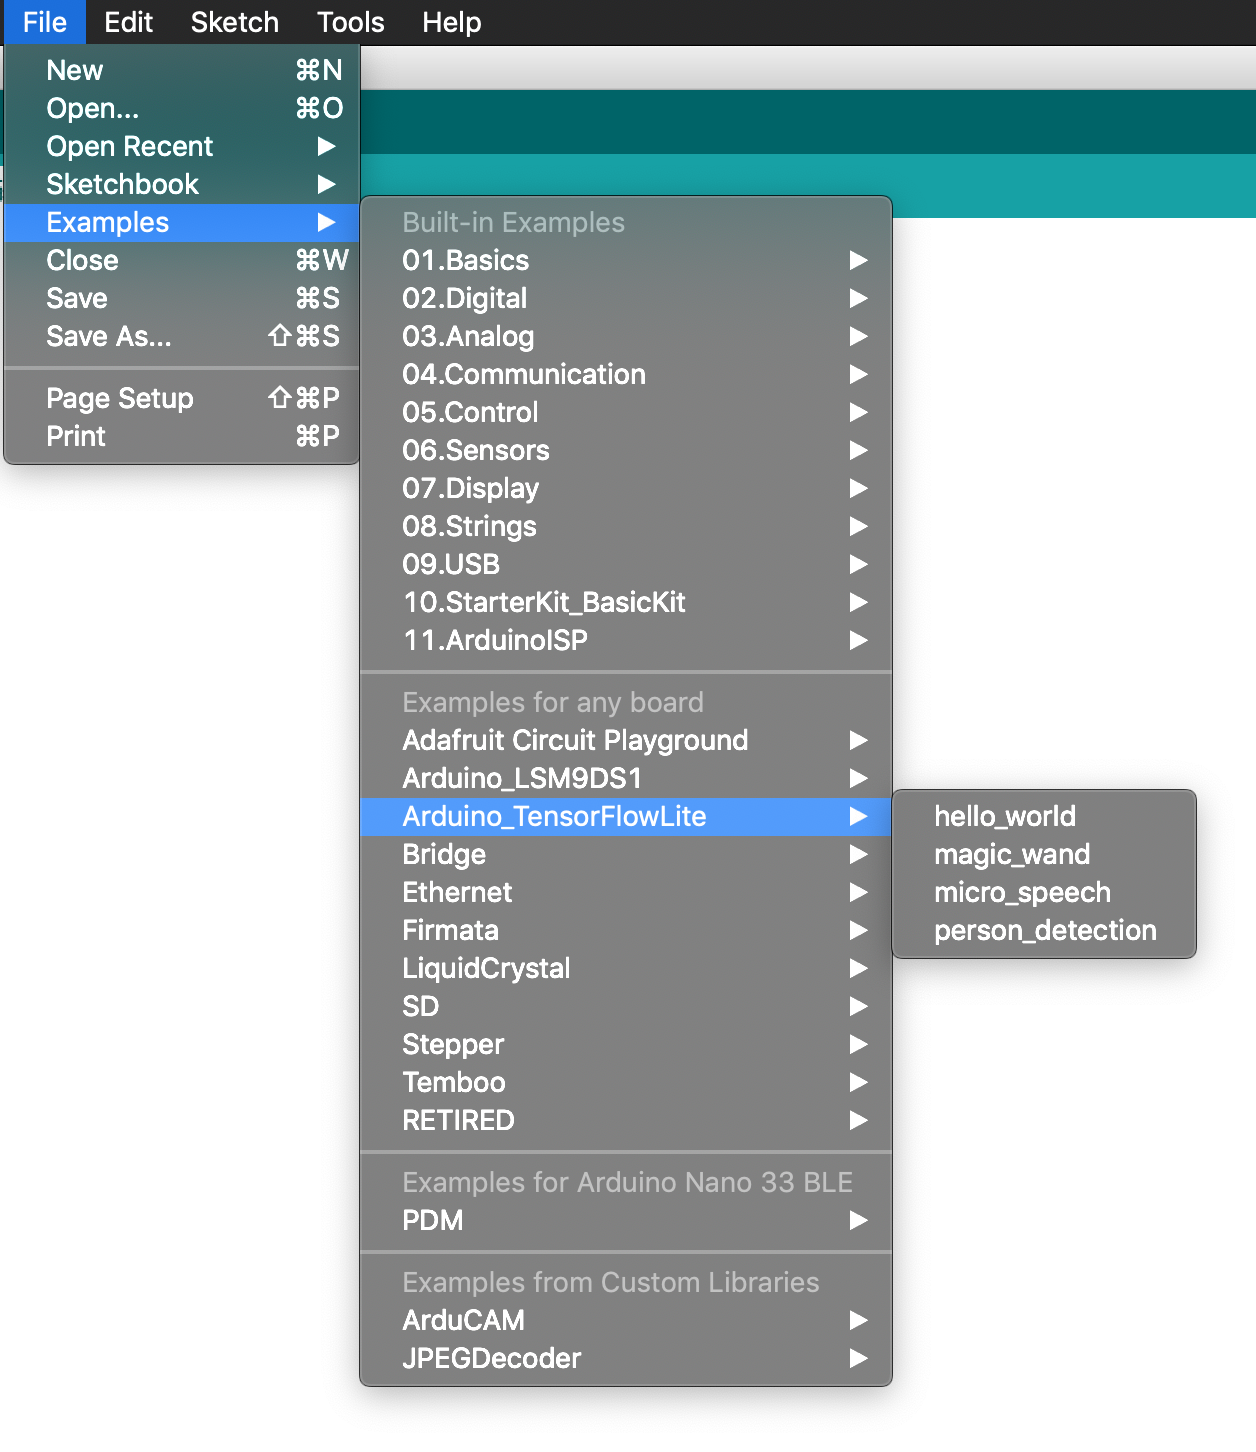
\includegraphics{Arduino/tinyML9-2}
  \caption{Screenshot des Menüs 'Examples'}\label{tinyML9-2}
\end{figure}



Klicken Sie auf \FILE{\glqq person\_detection\grqq}, um das Beispiel zu laden. Es erscheint ein neues Fenster mit einer Registerkarte für jede der Quelldateien. Die Datei in der ersten Registerkarte, \FILE{person\_detection}, entspricht der Datei \FILE{main\_functions.cc}, die wir zuvor durchgelesen haben.

\subsection{Bemerkung}

"Das Ausführen des Beispiels" hat bereits die Struktur des Arduino-Beispiels erklärt, daher werden wir es hier nicht noch einmal behandeln.

Zusätzlich zur TensorFlow-Bibliothek müssen wir zwei weitere Bibliotheken installieren:

\begin{enumerate}
  \item Die Bibliothek \FILE{Arducam}, damit unser Code mit der Hardware interagieren kann
  \item Die Bibliothek \FILE{JPEGDecoder}, damit wir JPEG-kodierte Bilder dekodieren können
\end{enumerate}

Die Arducam-Arduino-Bibliothek ist auf GitHub verfügbar. Um sie zu installieren, laden Sie das Repository herunter oder klonen Sie es. Kopieren Sie anschließend das Unterverzeichnis \FILE{ArduCAM} in Ihr Verzeichnis \FILE{Arduino/libraries}. Um das Bibliotheksverzeichnis auf Ihrem Rechner zu finden, überprüfen Sie den Sketchbook-Speicherort im Voreinstellungsfenster der Arduino IDE.

Nachdem Sie die Bibliothek heruntergeladen haben, müssen Sie eine ihrer Dateien bearbeiten, um sicherzustellen, dass sie für die Arducam Mini 2MP Plus konfiguriert ist. Öffnen Sie dazu \FILE{Arduino/libraries/ArduCAM/memorysaver.h}.

Sie sollten eine Reihe von \PYTHON{\#define}-Anweisungen aufgelistet sehen. Stellen Sie sicher, dass sie alle auskommentiert sind, außer \PYTHON{\#define OV2640\_MINI\_2MP\_PLUS}, wie hier gezeigt:

\begin{code}
    \begin{lstlisting}
//Step 1: select the hardware platform, only one at a time
//#define OV2640_MINI_2MP
//#define OV3640_MINI_3MP
//#define OV5642_MINI_5MP
//#define OV5642_MINI_5MP_BIT_ROTATION_FIXED
#define OV2640_MINI_2MP_PLUS
//#define OV5642_MINI_5MP_PLUS
//#define OV5640_MINI_5MP_PLUS
  \end{lstlisting}
\end{code}

Nachdem Sie die Datei gespeichert haben, sind Sie mit der Konfiguration der Arducam-Bibliothek fertig.

\subsection{Tip}

Das Beispiel wurde mit \SHELL{Commit \#e216049} der Arducam-Bibliothek entwickelt. Wenn Sie Probleme mit der Bibliothek haben, können Sie versuchen, diesen speziellen Commit herunterzuladen, um sicherzustellen, dass Sie genau denselben Code verwenden.

Der nächste Schritt ist die Installation der Bibliothek \FILE{JPEGDecoder}. Sie können dies aus der Arduino-IDE heraus tun. Wählen Sie im Menü "Tools" die Option "Manage Libraries" und suchen Sie nach \FILE{JPEGDecoder}. Sie sollten die Version 1.8.0 der Bibliothek installieren.

Nachdem Sie die Bibliothek installiert haben, müssen Sie sie konfigurieren, um einige optionale Komponenten zu deaktivieren, die nicht mit dem Arduino Nano 33 BLE Sense kompatibel sind. Öffnen Sie \FILE{Arduino/libraries/JPEGDecoder/src/User\_Config.h} und stellen Sie sicher, dass sowohl \PYTHON{\#define LOAD\_SD\_LIBRARY} als auch \PYTHON{\#define LOAD\_SDFAT\_LIBRAR} auskommentiert sind, wie in diesem Auszug aus der Datei gezeigt:

\begin{code}
    \begin{lstlisting}
// Comment out the next #defines if you are not using an SD Card to store
// the JPEGs
// Commenting out the line is NOT essential but will save some FLASH space if
// SD Card access is not needed. Note: use of SdFat is currently untested!

//#define LOAD_SD_LIBRARY // Default SD Card library
//#define LOAD_SDFAT_LIBRARY // Use SdFat library instead, so SD Card SPI can
// be bit bashed
  \end{lstlisting}
\end{code}

Nachdem Sie die Datei gespeichert haben, ist die Installation der Bibliotheken abgeschlossen. Sie sind nun bereit, die Anwendung zur Personenerkennung auszuführen!

Schließen Sie zunächst Ihr Arduino-Gerät über USB an. Vergewissern Sie sich, dass der richtige Gerätetyp in der Dropdown-Liste "Board" im Menü "Tools" ausgewählt ist, wie in Abbildung~\ref{tinyML9-3} gezeigt.

\begin{figure}
    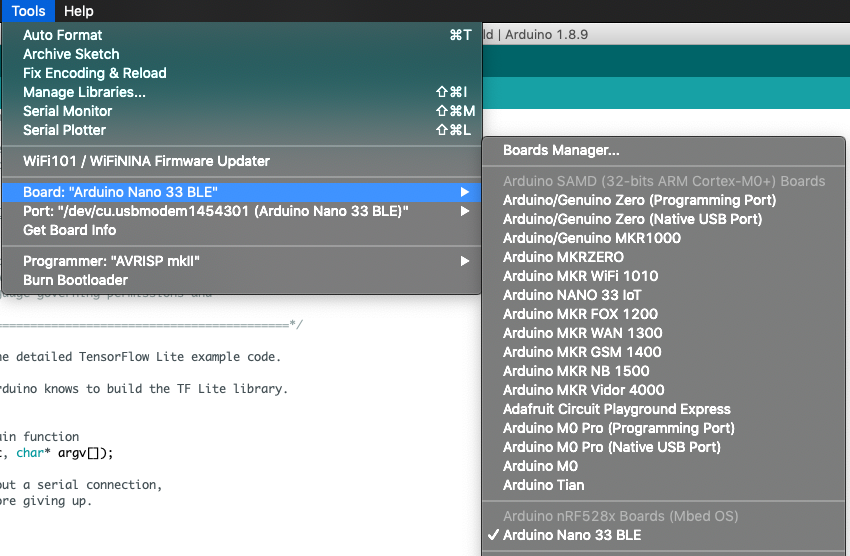
\includegraphics{Arduino/tinyML9-3}
    \caption{Screenshot of the 'Board' dropdown}\label{tinyML9-3}
\end{figure}


Wenn der Name Ihres Geräts nicht in der Liste erscheint, müssen Sie sein Support-Paket installieren. Klicken Sie dazu auf Boards Manager. Suchen Sie in dem daraufhin angezeigten Fenster nach Ihrem Gerät und installieren Sie die neueste Version des entsprechenden Support-Pakets.

Vergewissern Sie sich auch im Menü Tools, dass der Anschluss des Geräts in der Dropdown-Liste Port ausgewählt ist, wie in Abbildung~\ref{tinyML9-4} gezeigt.

\begin{figure}
    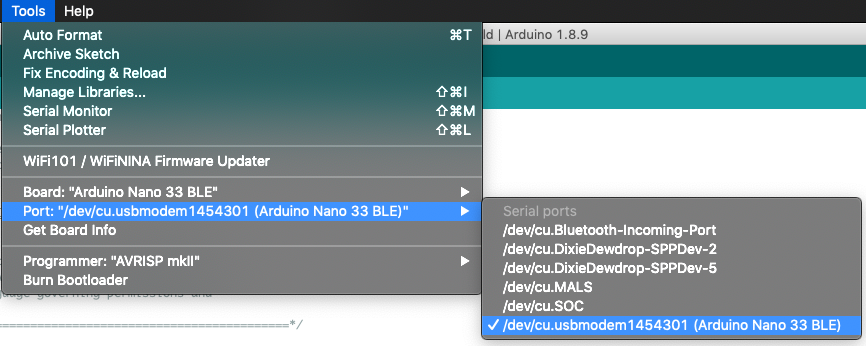
\includegraphics{Arduino/tinyML9-4}
    \caption{Screenshot of the 'Port' dropdown}\label{tinyML9-4}
\end{figure}


Klicken Sie schließlich im Arduino-Fenster auf die Schaltfläche "Hochladen" (in Abbildung~\ref{tinyML9-4} weiß hervorgehoben), um den Code zu kompilieren und auf Ihr Arduino-Gerät hochzuladen.


\begin{figure}
    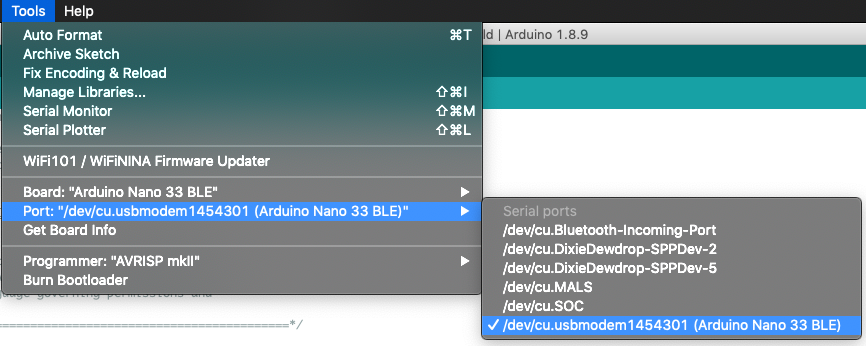
\includegraphics{Arduino/tinyML9-4}
    \caption{Screenshot of the upload button}\label{tinyML9-4}
\end{figure}

Sobald der Upload erfolgreich abgeschlossen ist, wird das Programm ausgeführt.

Um es zu testen, beginnen Sie damit, die Kamera des Geräts auf etwas zu richten, das definitiv keine Person ist oder nur das Objektiv verdeckt. Wenn die blaue LED das nächste Mal blinkt, nimmt das Gerät ein Bild von der Kamera auf und beginnt, die Inferenz auszuführen. Da das Bildverarbeitungsmodell, das wir für die Personenerkennung verwenden, relativ groß ist, wird die Inferenz sehr lange dauern - etwa 19 Sekunden zum Zeitpunkt des Schreibens, obwohl es möglich ist, dass TensorFlow Lite seitdem schneller geworden ist.

Wenn die Inferenz abgeschlossen ist, wird das Ergebnis in eine weitere leuchtende LED übersetzt. Sie haben die Kamera auf etwas gerichtet, das keine Person ist, also sollte die rote LED aufleuchten.

Versuchen Sie nun, die Kamera des Geräts auf sich selbst zu richten! Wenn die blaue LED das nächste Mal blinkt, nimmt das Gerät ein weiteres Bild auf und beginnt, die Inferenz durchzuführen. Nach etwa 19 Sekunden sollte die grüne LED aufleuchten.

Denken Sie daran, dass die Bilddaten vor jeder Inferenz als Schnappschuss aufgenommen werden, wenn die blaue LED blinkt. Das, worauf die Kamera in diesem Moment gerichtet ist, wird in das Modell eingespeist. Es spielt keine Rolle, worauf die Kamera gerichtet ist, bis das nächste Mal ein Bild aufgenommen wird, wenn die blaue LED wieder blinkt.

Wenn Sie scheinbar falsche Ergebnisse erhalten, stellen Sie sicher, dass Sie sich in einer Umgebung mit guter Beleuchtung befinden. Sie sollten auch sicherstellen, dass die Kamera richtig ausgerichtet ist, mit den Stiften nach unten, so dass die Bilder, die sie aufnimmt, richtig herum sind - das Modell wurde nicht darauf trainiert, auf dem Kopf stehende Personen zu erkennen. Außerdem sollten Sie bedenken, dass es sich um ein winziges Modell handelt, bei dem die Genauigkeit gegen die geringe Größe eingetauscht wird. Es funktioniert sehr gut, aber es ist nicht immer zu 100 % genau.

Sie können die Ergebnisse der Inferenz auch über den Arduino Serial Monitor sehen. Öffnen Sie dazu im Menü "Tools" den "Serial Monitor". Sie werden ein detailliertes Protokoll sehen, das zeigt, was passiert, während die Anwendung läuft. Es ist auch interessant, das Kästchen "Show timestamp" (Zeitstempel anzeigen) zu aktivieren, damit Sie sehen können, wie lange jeder Teil des Prozesses dauert:




\begin{code}
    \begin{lstlisting}
14:17:50.714 -> Starting capture
14:17:50.714 -> Image captured
14:17:50.784 -> Reading 3080 bytes from ArduCAM
14:17:50.887 -> Finished reading
14:17:50.887 -> Decoding JPEG and converting to greyscale
14:17:51.074 -> Image decoded and processed
14:18:09.710 -> Person score: 246 No person score: 66
  \end{lstlisting}
\end{code}

Aus diesem Protokoll ist ersichtlich, dass das Erfassen und Lesen der Bilddaten vom Kameramodul ca. 170 ms, das Dekodieren des JPEGs und die Umwandlung in Graustufen 180 ms und die Durchführung der Inferenz 18,6 Sekunden dauerte.

\subsection{Ausführung von Änderungen}

Jetzt, wo Sie die Basisanwendung bereitgestellt haben, können Sie ein wenig herumspielen und einige Änderungen am Code vornehmen. Bearbeiten Sie einfach die Dateien in der Arduino-IDE und speichern Sie sie, und wiederholen Sie dann die vorherigen Anweisungen, um den geänderten Code auf dem Gerät einzusetzen.

Hier sind ein paar Dinge, die Sie ausprobieren können:

\begin{itemize}
  \item Ändern Sie den Erkennungsresponder so, dass er mehrdeutige Eingaben ignoriert, bei denen es keinen großen Unterschied zwischen den Bewertungen "Person" und "keine Person" gibt.
\item Verwenden Sie die Ergebnisse der Personenerkennung, um andere Komponenten zu steuern, z. B. zusätzliche LEDs oder Servos.
\item Bauen Sie eine intelligente Sicherheitskamera, indem Sie Bilder speichern oder übertragen - aber nur solche, die eine Person enthalten.
\end{itemize}





















\cite{Chowdhery:2019}


\url{https://github.com/tensorflow/tensorflow/tree/master/tensorflow/lite/micro/examples/person\_detection}

\subsection{Laufen auf Arduino}

Die folgenden Anweisungen helfen Ihnen, dieses Beispiel zu erstellen und auf Arduino-Geräten einzusetzen.

Das Beispiel wurde mit dem folgenden Gerät getestet:

Arduino Nano 33 BLE Sense
Sie benötigen außerdem das folgende Kameramodul:

Arducam Mini 2MP Plus

Hardware
Schließen Sie die Pins der Arducam wie folgt an:

\begin{tabular}{ll}
  Arducam pin name & Arduino pin name \\ \hline
  CS               & D7 (unlabelled, immediately to the right of D6) \\
  MOSI             & D11 \\
  MISO             & D12 \\
  SCK              & D13 \\
  GND              & GND (either pin marked GND is fine) \\
  VCC              & 3.3 V \\
  SDA              & A4 \\
  SCL              & A5 \\
\end{tabular}

Installieren Sie die Bibliothek \FILE{Arduino\_TensorFlowLite}

Laden Sie den aktuellen nächtlichen Build der Bibliothek herunter: \FILE{person\_detection.zip}

Diese Beispielanwendung ist als Teil der offiziellen TensorFlow Lite Arduino-Bibliothek enthalten. Um sie zu installieren, öffnen Sie den Arduino Bibliotheksmanager in Tools -> Manage Libraries... und suchen Sie nach \FILE{Arduino\_TensorFlowLite}.

\subsection{Installation anderer Bibliotheken}

Zusätzlich zur TensorFlow-Bibliothek müssen Sie noch zwei weitere Bibliotheken installieren:

Die Arducam-Bibliothek, damit unser Code mit der Hardware kommunizieren kann
Die JPEGDecoder-Bibliothek, so dass wir JPEG-kodierte Bilder dekodieren können
Die Arducam-Arduino-Bibliothek ist auf GitHub unter \url{https://github.com/ArduCAM/Arduino} verfügbar. Um sie zu installieren, laden Sie das Repository herunter oder klonen Sie es. Kopieren Sie anschließend das Unterverzeichnis ArduCAM in Ihr Arduino/libraries-Verzeichnis. Um dieses Verzeichnis auf Ihrem Rechner zu finden, überprüfen Sie den Sketchbook-Speicherort im Fenster "Einstellungen" der Arduino IDE.

Nachdem Sie die Bibliothek heruntergeladen haben, müssen Sie eine ihrer Dateien bearbeiten, um sicherzustellen, dass sie für die Arducam Mini 2MP Plus konfiguriert ist. Öffnen Sie dazu die folgende Datei:

\FILE{Arduino/libraries/ArduCAM/memorysaver.h}

You'll see a bunch of \PYTHON{\#define} statements listed. Make sure that they are all commented out, except for \PYTHON{\#define OV2640\_MINI\_2MP\_PLUS}, as so:

\begin{code}
    \begin{lstlisting}
//Step 1: select the hardware platform, only one at a time
//#define OV2640_MINI_2MP
//#define OV3640_MINI_3MP
//#define OV5642_MINI_5MP
//#define OV5642_MINI_5MP_BIT_ROTATION_FIXED
#define OV2640_MINI_2MP_PLUS
//#define OV5642_MINI_5MP_PLUS
//#define OV5640_MINI_5MP_PLUS
  \end{lstlisting}
\end{code}

Sobald Sie die Datei gespeichert haben, sind wir mit der Konfiguration der Arducam-Bibliothek fertig.

Unser nächster Schritt ist die Installation der JPEGDecoder-Bibliothek. Wir können dies aus der Arduino-IDE heraus tun. Gehen Sie zunächst auf die Option "Manage Libraries..." im Menü "Tools" und suchen Sie nach JPEGDecoder. Sie sollten die Version 1.8.0 der Bibliothek installieren.

Sobald die Bibliothek installiert ist, müssen wir sie konfigurieren, um einige optionale Komponenten zu deaktivieren, die nicht mit dem Arduino Nano 33 BLE Sense kompatibel sind. Öffnen Sie die folgende Datei:

\FILE{Arduino/libraries/JPEGDecoder/src/User\_Config.h}

Stellen Sie sicher, dass sowohl \PYTHON{\#define LOAD\_SD\_LIBRARY} als auch \PYTHON{\#define LOAD\_SDFAT\_LIBRARY} auskommentiert sind, wie in diesem Auszug aus der Datei gezeigt:


\begin{code}
    \begin{lstlisting}
// Comment out the next #defines if you are not using an SD Card to store the JPEGs
// Commenting out the line is NOT essential but will save some FLASH space if
// SD Card access is not needed. Note: use of SdFat is currently untested!

//#define LOAD_SD_LIBRARY // Default SD Card library
//#define LOAD_SDFAT_LIBRARY // Use SdFat library instead, so SD Card SPI can be bit bashed-device, then build and upload the example.
  \end{lstlisting}
\end{code}



Um die Kamera zu testen, beginnen Sie damit, die Kamera des Geräts auf etwas zu richten, das definitiv keine Person ist, oder sie einfach zu verdecken. Wenn die blaue LED das nächste Mal blinkt, erfasst das Gerät ein Bild von der Kamera und beginnt mit der Inferenz. Das Bildverarbeitungsmodell, das wir für die Personenerkennung verwenden, ist relativ groß, aber mit den cmsis-nn-Optimierungen dauert es nur etwa 800 ms, um das Modell auszuführen.

Nach einem Moment wird das Ergebnis der Inferenz in das Aufleuchten einer weiteren LED umgesetzt. Da Sie die Kamera auf etwas gerichtet haben, das keine Person ist, sollte die rote LED aufleuchten.

Versuchen Sie nun, die Kamera des Geräts auf sich selbst zu richten! Wenn die blaue LED das nächste Mal blinkt, nimmt das Gerät ein weiteres Bild auf und beginnt, die Inferenz durchzuführen. Nach einer kurzen Pause sollte die grüne LED aufleuchten!

Denken Sie daran, dass die Bilddaten vor jeder Inferenz als Schnappschuss aufgenommen werden, wenn die blaue LED blinkt. Das, worauf die Kamera in diesem Moment gerichtet ist, wird in das Modell eingespeist. Es spielt keine Rolle, wohin die Kamera gerichtet ist, bis das nächste Mal ein Bild aufgenommen wird, wenn die blaue LED wieder blinkt.

Wenn Sie scheinbar falsche Ergebnisse erhalten, stellen Sie sicher, dass Sie sich in einer Umgebung mit guter Beleuchtung befinden. Sie sollten auch sicherstellen, dass die Kamera richtig ausgerichtet ist, mit den Stiften nach unten, so dass die Bilder, die sie aufnimmt, richtig herum sind - das Modell wurde nicht darauf trainiert, auf dem Kopf stehende Personen zu erkennen! Außerdem sollte man bedenken, dass es sich um ein winziges Modell handelt, bei dem die Genauigkeit gegen die geringe Größe eingetauscht wird. Es funktioniert sehr gut, aber es ist nicht immer zu 100 % genau.

Wir können die Ergebnisse der Inferenz auch über den Arduino Serial Monitor sehen. Dazu öffnen Sie den Serial Monitor aus dem Menü Tools. Sie werden ein detailliertes Protokoll dessen sehen, was passiert, während unsere Anwendung läuft. Es ist auch interessant, das Kontrollkästchen Zeitstempel anzeigen zu aktivieren, so dass Sie sehen können, wie lange jeder Teil des Prozesses dauert:



\begin{code}
    \begin{lstlisting}
14:17:50.714 -> Starting capture
14:17:50.714 -> Image captured
14:17:50.784 -> Reading 3080 bytes from ArduCAM
14:17:50.887 -> Finished reading
14:17:50.887 -> Decoding JPEG and converting to greyscale
14:17:51.074 -> Image decoded and processed
14:18:09.710 -> Person score: 246 No person score: 66
  \end{lstlisting}
\end{code}

Aus dem Protokoll geht hervor, dass etwa 170 ms für die Erfassung und das Lesen der Bilddaten vom Kameramodul, 180 ms für die Dekodierung des JPEGs und die Umwandlung in Graustufen und 18,6 Sekunden für die Inferenz benötigt wurden.


\chapter{Hardware the Arduino Nano 33 BLE Sense}

\section{Indroduction}

Arduino has a wide range of Integrated circuit family, depending upon the requirenment and usage. The most commonly available arduino family boards are MKR Family, Arduino Classis, Nano fmaily, Pro Family, and Nicla Family. Each arduino family have further multiple types of boards, e.g the Nano family has a following boards; Nano Classic, Nano 33 BLE, Nano 33 BLE Sense, Nano 33 IoT, and Nano Every, each has a unique specification. The Arduino development board is based on a microcontroller with a large number of standard electronic components and an open source schematic that can be modified as needed.

The BLE (Bluetooth Low Energy) compact and reliable Nano board are built on NINA B306 module for BLE and Bluetooth 5 communication; the NINA B306 module based on Nordic nRF52480 processor that contains a powerful Cortex M4F CPU, Its architecture fully compatible with Arduino IDE Online and Offline. The figure ~\ref{fig:abx00031front12} shows, the Arduino Nano BLE 33 Sense have a following set of sensors on board, ADPS-9960, LPS22HB, HTS221, LSM9DS1,and MP34DT05-A. It is small in size, having all the required sensor on board. \cite{ArduinoNano33:2021}



\begin{figure}[ht]
	\centering
	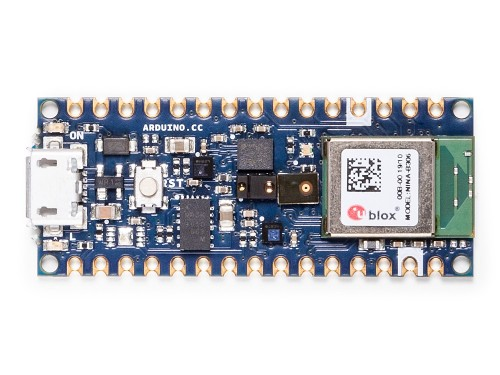
\includegraphics[width=0.5\linewidth]{Nano33BLESense/abx00031_front_1_2}
	\caption{Arduino Nano 33 BLE}
	\label{fig:abx00031front12}
\end{figure}

The Arduino Nano 33 BLE Sense have the following set of Sensors, BLE module and its functionality below.

\begin{itemize}
	\item The Bluetooth is managed by a NINA B306 module.
	\item The ADPS-9960 is a digital proximity, ambient light, RGB and gesture sensor.
	\item The LSM9DS1 is a system-in-package featuring a 3D digital linear acceleration sensor, a 3D digital angular rate sensor, and a 3D digital magnetic sensor.
	\item The LPS22HB reads barometric pressure and environmental temperature.
	\item The HTS221 senses relative humidity.
	\item The MP34DT05 is support the sound detection.
\end{itemize}

\section{On Board Sensors and its Functionality}

\subsection{ADPS-9960 (Gesture, Proximity, and Color Detection Sensor)}

The APDS-9960 device features advanced Gesture detection, Proximity detection, Digital Ambient Light Sense (ALS) and Color Sense (RGB). \cite{ArduinoNano33:2021} Gesture detection utilizes four directional photodiodes to sense reflected IR energy (sourced by the integrated LED) to convert physical motion information (i.e. velocity, direction and distance) to a digital information.



\textbf{Applications}

\begin{itemize}
  \item Gesture Detection
  \item Color Sense
  \item Ambient Light Sensing
  \item Proximity Sensing
\end{itemize}

\subsection{LSM9DS1 (Accelerometer, Gyroscope, and Magnetometre)}
The LSM9DS1 is a system-in-package featuring a 3D digital linear acceleration sensor, a 3D digital angular rate sensor, and a 3D digital magnetic sensor.

\textbf{Aplications}

\begin{itemize}
  \item Indoor navigation
  \item Advanced gesture recognition
  \item Gaming and virtual reality input devices
  \item Display/map orientation and browsing
\end{itemize}
  
\subsection{LPS22HB (Pressure Sensor)}
The LPS22HB is an ultra-compact piezoresistive absolute pressure sensor which functions as a
digital output barometer.

\textbf{Applications}


\begin{itemize}
  \item Altimeters and barometers for portable devices 
  \item Weather station equipment
  \item Sports watchs
\end{itemize}

\subsection{HTS221 (Relative Humidity and Temperature)}
The HTS221 is an ultra-compact sensor for relative humidity and temperature. It includes a sensing element and a mixed signal to provide the measurement information through digital serial interfaces.

\textbf{Applications}

\begin{itemize}
  \item Air conditioning, heating and ventilation 
  \item Air humidifiers
  \item Refrigerators
  \item Smart home automation
  \item Industrial automation
\end{itemize}  


\subsection{MP34DT05-A (Digital Microphone)}

The MP34DT05-A is an ultra-compact, low-power, omni directional, digital microphone built with a capacitive sensing element and an IC interface. The sensing element, capable of detecting acoustic waves, is manufactured using a specialized silicon micromachining process dedicated to producing audio sensors.

\textbf{Applications}

\begin{itemize}
  \item Speech recognition 
  \item Portable media player
  \item Mobile Terminal
\end{itemize}


\subsection{nRF52840 (Bluetooth Module)}

The nRF52840 is an advanced, highly flexible single chip solution for today’s increasingly demanding Ultra low power (ULP) wireless applications for connected devices on our person, connected living environments and the IoT at large. It is designed ready for the major feature
advancements of Bluetooth 5 and takes advantage of Bluetooth 5’s increased performance capabilities. \cite{Arduino:2021b}

\textbf{Applications}

\begin{itemize}
  \item Smart Home products
  \item Industrial mesh networks
  \item Smart city infrastructure
  \item Connected watches
  \item Advanced personal fitness devices
  \item Wearables with wireless payment
  \item Connected Health
\end{itemize}

The Arduino 33 BLE Sense has a wide range of application, by having the set of sensors and Bluetooth low energy (BLE) capability, the communication becomes easy over the Bluetooth. Arduino Nano 33 BLE Sense operate on 3.3 V, so it make sure that do not apply 5v as normally the other boards need to operate. Also, for making the RGB color and person detection, we need to make the interface of Ble 33 Sense with Arducam OV2640 (Camera Shield). The Arducam OV2640 camera use  to detect the RGB, object detetion and also the gesture too. Arduino Nano 33 BLE Sense and Arducam (camera shield) is a perfect mactch for making ML and AI application, by having the set of sensors on board we just need to install the respective library on Arduino boar and it support the funcnality of sensors and Machine learning application.

\section{Arduino Nano 33 BLE Pin Configuration}

Arduino Nano 33 BLE is an advanced version of Arduino Nano board that is based on a powerful processor the nRF52840. The figure ~\ref{Schnittstellen} shows that the board has the following pin configuration. \href{https://www.etechnophiles.com/arduino-nano-33-ble-sense-pinout-introduction-specifications/}{Pin Configuration}

\textbf{Digital pin:}

The number of digital I/O pins are 14 which receive only two values HIGH or LOW. These pins can either be used as an input or output based on the requirement. When these pins receive 5V, they are in a HIGH state and when they receive 0V they are in a LOW state.

\textbf{Analog pin}

Total 8 analog pins available on the board A0 – A7. These pins get any value as opposed to digital pins that only receive two values HIGH or LOW. These pins are used to measure the analog voltage ranging between 0 to 5V.


\textbf{PWM pin}

All digital pins can be used as PWM pins. These pins generate analog results with digital means.


\textbf{SPI pin}

The board supports serial peripheral interface (SPI) communication protocol. This protocol is employed to develop communication between a controller and other peripheral devices like shift registers and sensors. Two pins are used for SPI communication i.e. Master Input Slave Output (MISO) and Master Output Slave Input (MOSI) are used for SPI communication. These pins are used to send or receive data by the controller.

\textbf{I2C pin}

The board carries the I2C communication protocol which is a two-wire protocol. It comes with two pins SDL and SCL.

\textbf{UART pin}

The board features a UART communication protocol that is used for serial communication and carries two pins Rx and Tx. The Rx is a receiving pin used to receive the serial data while Tx is a transmission pin used to transmit the serial data.


\textbf{External Interrupts pin}

All digital pins can be used as external interrupts. This feature is used in case of emergency to interrupt the main running program with the inclusion of important instructions at that point.

\textbf{LED at Pin 13 and AREF pin}

There is an LED connected to pin 13 of the board. And AREF is a pin used as a reference voltage for the input voltage.



\begin{figure}[ht]
	\centering
	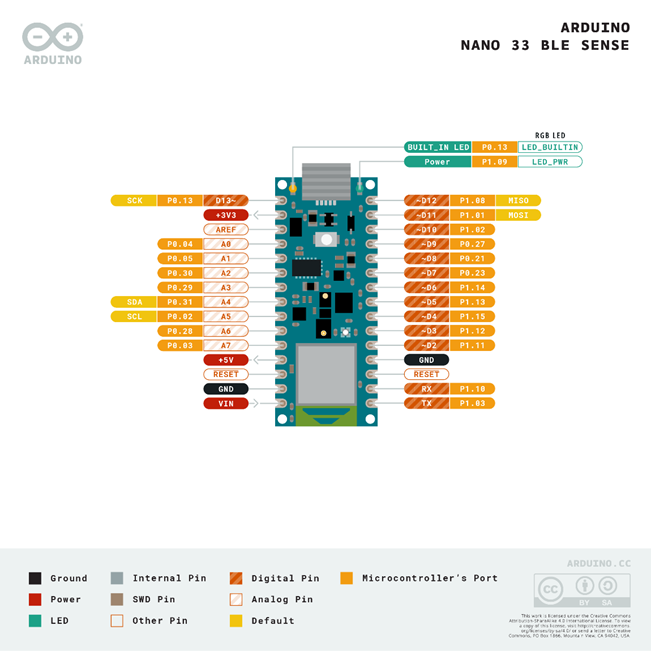
\includegraphics[width=0.5\linewidth]{Nano33BLESense/Schnittstellen}
	\caption{Arduino Nano 33 BLE Pin Configuration}
	\label{Schnittstellen}
\end{figure}


\chapter{ArduCAM OV2640}

\section{Indroduction}

ArduCAM is Arduino based open source camera platform which is well mated to Arduino boards. It is a high definition 2MP SPI camera, which reduce the complexity of the camera control interface. It integrates 2MP CMOS image sensor OV2640, and provides miniature size, as well as the easy to use hardware interface and open source code library. The ArduCAM mini can be used in any platforms like Arduino, Raspberry Pi, Maple, Chipkit, Beaglebone black, as long as they have SPI and I2C interface and can be well mated with standard Arduino boards. The figure ~\ref{Arducam} shows the mini ArduCAM Camera. The mini ArduCAM OV2640 is well suited for tinyML application, it is easy to configure with Arduino boards. For making the ML applications, especially Images caputuring, object and gesture detection, it supports to take capture and send back to Arduino microcontroller for getting desire results. \href{https://www.arducam.com/product/arducam-2mp-spi-camera-b0067-arduino/}{[Arducam]}

\begin{figure}[ht]
	\centering
	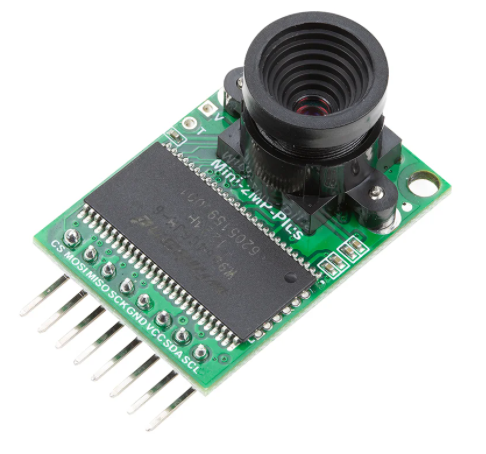
\includegraphics[width=0.5\linewidth]{Nano33BLESense/Arducam 2}
	\caption{ArduCAM interface with Arduino}
	\label{Arducam}
\end{figure}

\subsection{Pin Configuration of Arducam 0V2640 2MP Mini}

Arducam Mini 2MP OV2640 is a small mini size camera, we can easily embed this camera with any kind of Arduino or other electronics boards, if they have the serial peripheral interface (SPI) and  chip select (CS) . It has has 8 pins, the following figure ~\ref{pin config} shows the functionality of each pin.

\begin{figure}[ht]
	\centering
	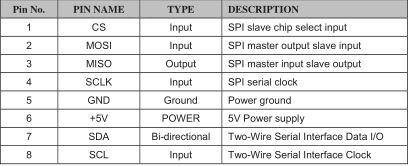
\includegraphics[width=0.8\linewidth]{Nano33BLESense/pin config}
	\caption{ArduCAM Pin Config}
	\label{pin config}
\end{figure}

It offers to add a camera interface with microcontroller the one who dont have camera capability, also there is a option to add multiple cameras with microcontroller.

\section{ArduCAM Interface with Arduino}

ArduCAM OV2640 needs the  SPI and I2C connection with the arduino boards. It will be connecting untill these two connections are make sure. The figure ~\ref{1} shows the ArduCAM connection with Arduino Mega 2560, the same connection will need with the other arduino boards too untill the availabity of  SPI and I2C connection. These ArduCAM cameras are easy to configure with arduino and depends upon the application, it is possible to connect multiple camera with sigle board to make the edge computing application. \href{https://www.arducam.com/product/arducam-2mp-spi-camera-b0067-arduino/}{Arducam Interface}

\begin{figure}[ht]
	\centering
	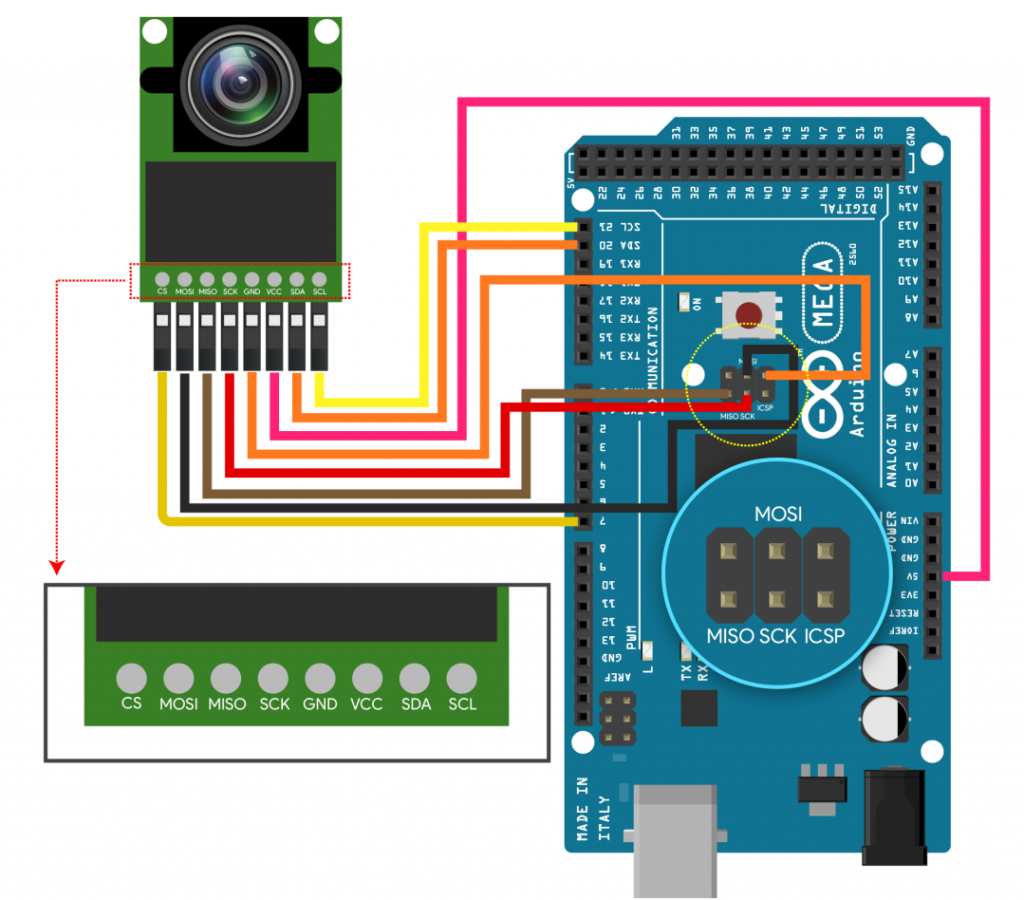
\includegraphics[width=0.6\linewidth]{Nano33BLESense/1}
	\caption{ArduCAM Interface with Arduin Mega 2560} 
	\label{1}
\end{figure}

ArduCAM is very small in size, even it is possible to fix the camera on the Arduino board. There is no external battery require for ArduCam to operate, It needs 5V/70mA operating power supply, so it will get the power from the arduino board too. By having the innovative funcnality with arduino boards, this can be use in the following applications.

\textbf{Application}

\begin{itemize}
  \item IOT Cameras
  \item Robot Cameras
  \item Wildlife Cameras
\end{itemize}  


\chapter{Software}

\section{Arduino IDE on PC}

\subsection{Installation}

Arduino Nano 33 BLE Sense can provide an energy-efficient and cost-effective solution for manufacturers who want to use Bluetooth Low Energy connectivity in their projects.\\

Arduino Nano 33 BLE Sense uses the Arduino software integrated development environment (IDE) for programming, which is the most widely used and common (IDE) for all arduino boards that can be run online and offline. This is a open-source Arduino Software (IDE) makes it easy to write code and upload it to the board. There are various version of software which is supported for each operating system (OS) e.g: mac, linux, and windows. Arduino community also provide us to start coding online and save our sketches in the cloud, this online arduino editor is most up-to-date version of the IDE includes all libraries and also supports new Arduino boards. For getting access to these software packages go to the following link \url{https://www.arduino.cc/en/software}  and get more up to date inforamtion, because every single day there are some updates occurs which is available on the link mention above. These software can be used with any Arduino board, the most recent offline arduino IDE 1.8.15 can be seen in Figure, \ref{fig:arduino-creat-agent-installieren} it is also supportive for all operating systems.

\begin{figure}[h]
	\centering
	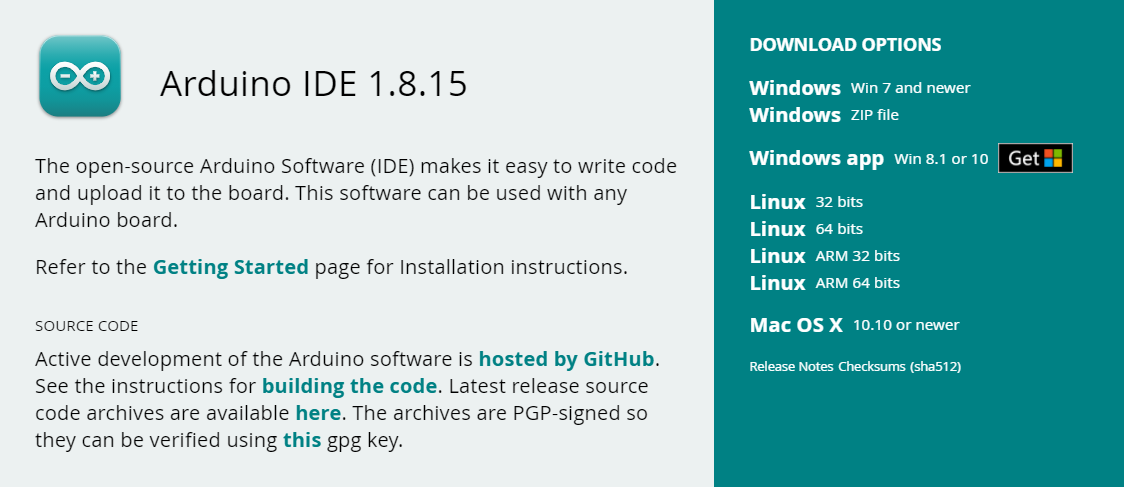
\includegraphics[width=1.0\linewidth]{Nano33BLESense/Installation-1}
	\caption{Arduino Creat Agent Installation}
	\label{fig:arduino-creat-agent-installieren}
\end{figure}


\subsection{Configuration}

To program the Arduino Nano 33 BLE Sense in offline state, we need to install one of the latest arduino IDE on our desktop. After installation, for getting access to the Arduino nano 33 ble sense board, we need to make configuration in our IDE. By opening the IDE, go to tool which can be seen on the uper left corner in IDE, in the tool there is an option for managed board. At this point we need to write our board name in the search which is Arduino Nano 33 BLE Sense as shown in figure, \ref {fig:Arduino-Mbed-Boards Installation} select the Arduino Mbed OS Boards and install it. The Mbed OS nano board supports also other nano family boards including Arduino nano 33 ble sense, after installing simply connect the Arduino Nano 33 BLE Sense to the computer via USB cable. 

\begin{figure}[h]
	\centering
	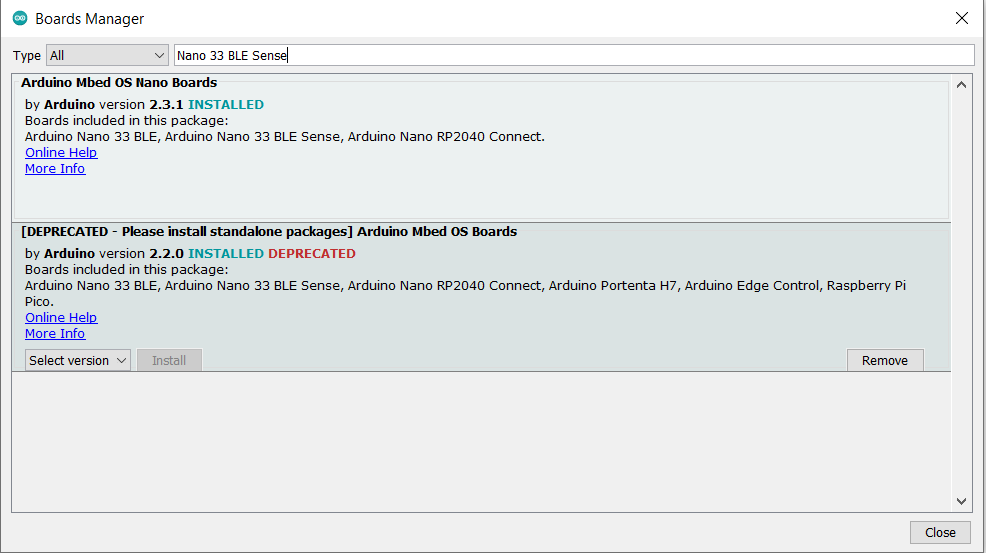
\includegraphics[width=1.0\linewidth]{Nano33BLESense/Nano Mbed}
	\caption{Arduino Mbed OS Nano Boards Installation}
	\label{fig:Arduino-Mbed-Boards Installation}
\end{figure}


\subsection{Test Example}

There are set of examples which are build in Arduino (IDE) for the testing purpose, for checking all the configuration and setting up the board we can open one of the basic LED blink example first as shown in the figure.  \ref{fig:LED-Example}.

\begin{figure}[h]
	\centering
	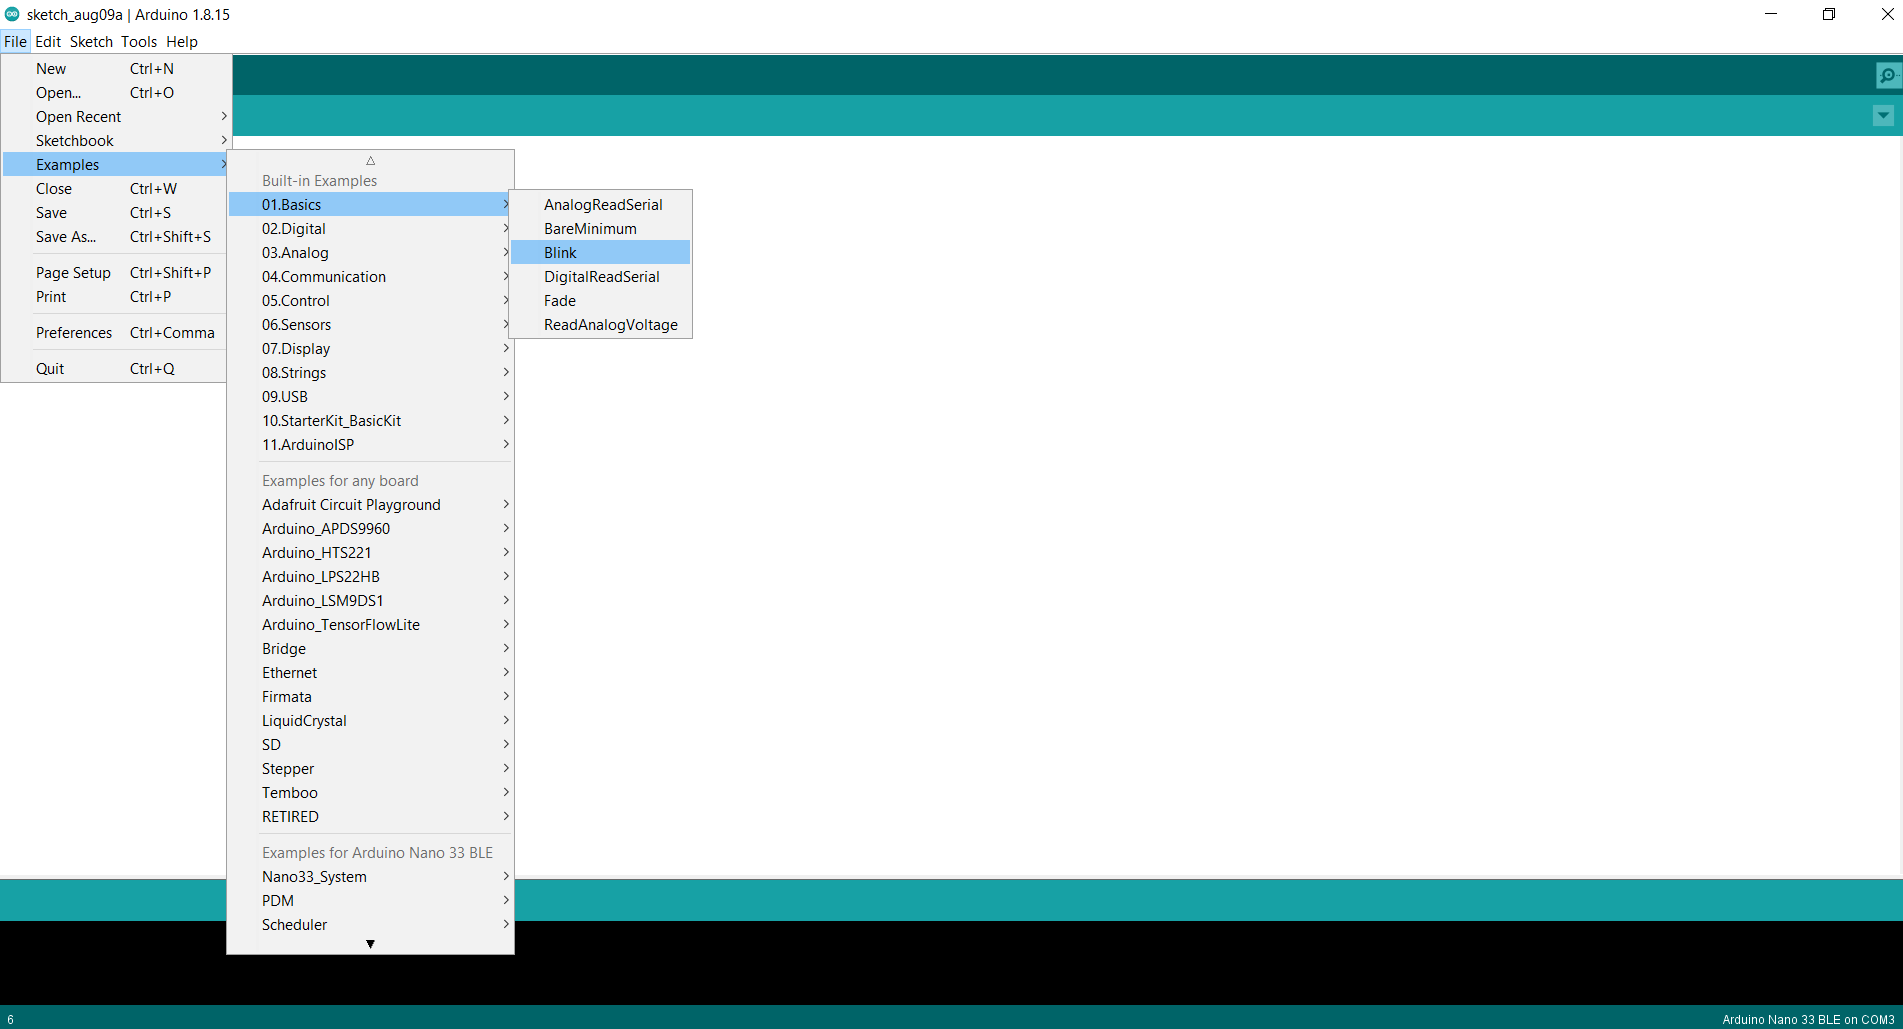
\includegraphics[width=1.0\linewidth]{Nano33BLESense/LED}
	\caption{LED-Example Test}
	\label{fig:LED-Example}
\end{figure}

This LED-blink example support all the arduino boards, for the checking purposes just need to run this basic example on any arduino embed board and it will blink the LED on our Arduino board after pre-set miliseconds. In the same example folder, there are also number of build in usefull example written in Arduino IDE for embedded boards. These examples are very usefull for getting the basic knowledge about the board and programming.

\section{Pre-requisite settings for Uploading the program}

There are some pre-requisite steps need to follow either we need to run the build in example or run by our own written program. By operating the Arduino board with Laptop with the help of USB connection, need to open the Arduino IDE on desktop, it appears a blank arduino environment page just a Void setup and void loop written on it. At this step we need to go to the tool-Arduino board and select the connected board which is Arduino Nano 33 Ble Sense as shown in the figure \ref{fig:Check Board}

\begin{figure}[h]
	\centering
	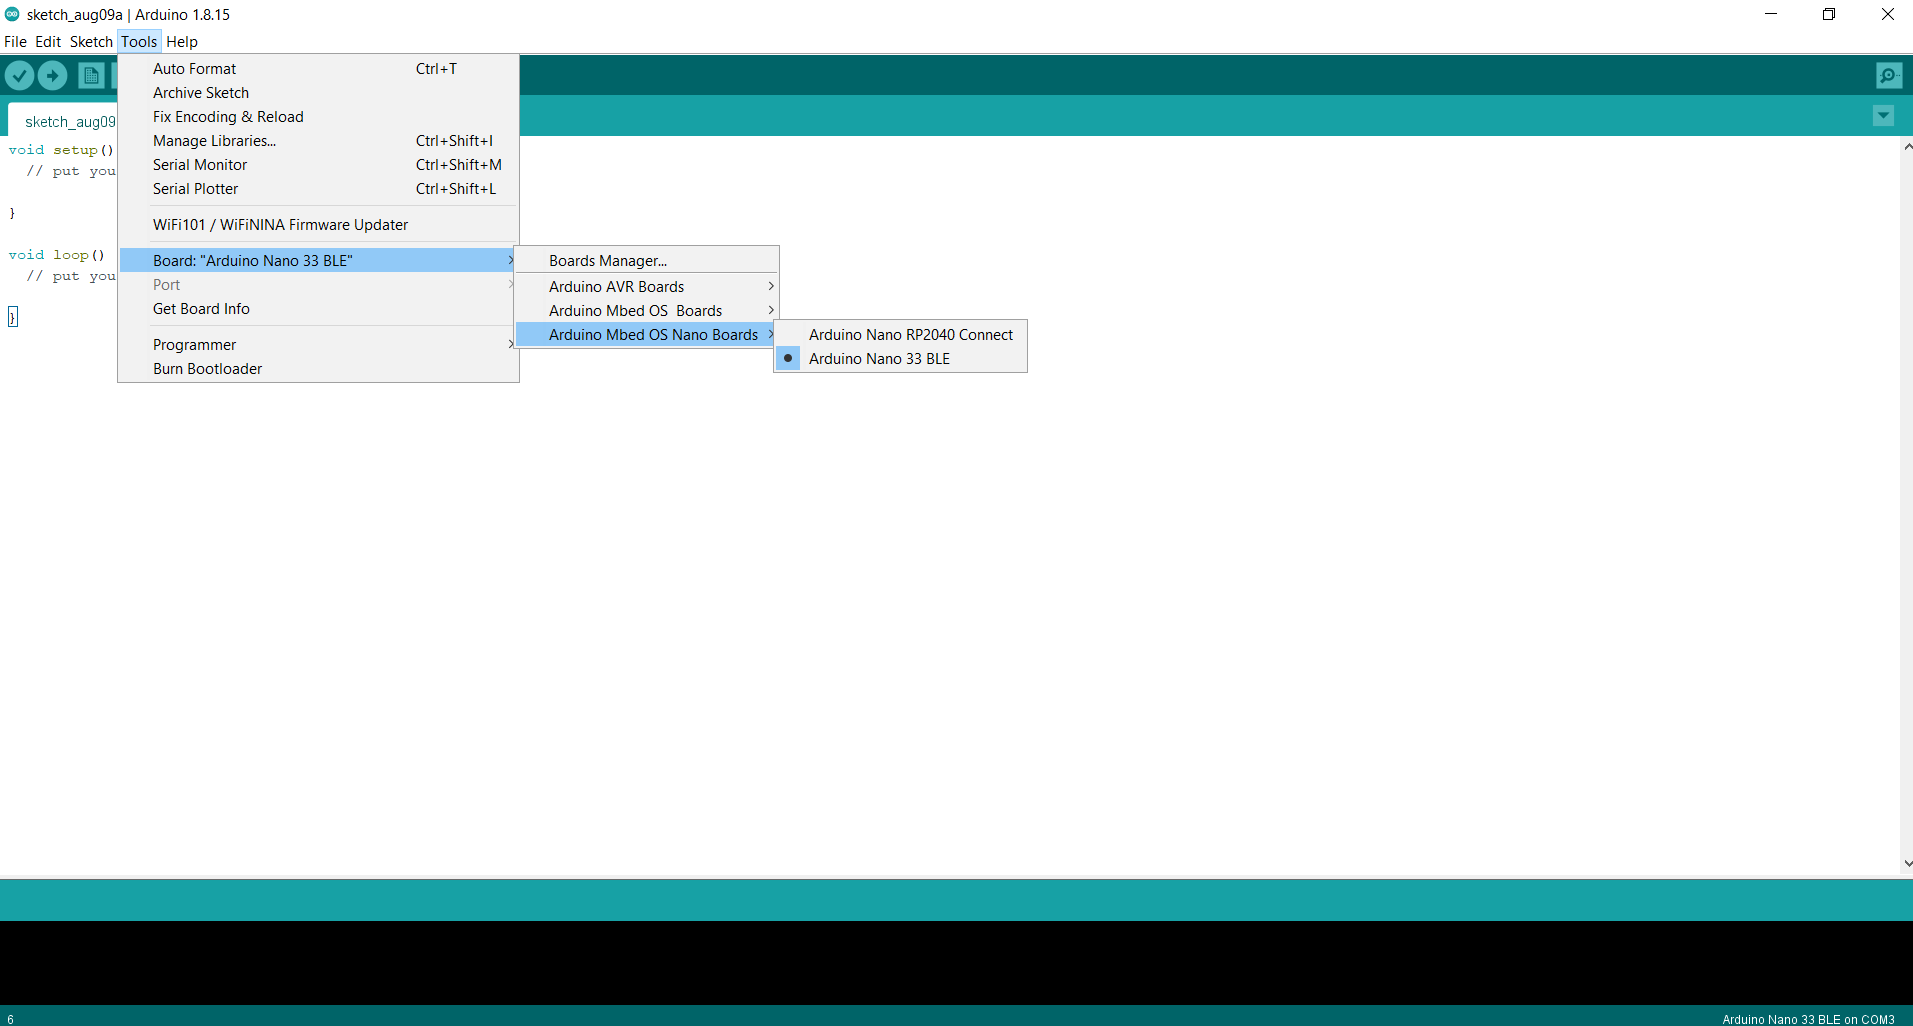
\includegraphics[width=1.0\linewidth]{Nano33BLESense/Check-board}
	\caption{Select the Connected board}
	\label{fig:Check Board}
\end{figure}

\subsection{Select the Appropriate Port}

By selecting the Arduino nano 33 BLE sense board, next we need to check the connected port. For doing this, we need to set our arduino borad in Boot setup by clicking the white reset button on arduino as show in figure\ref{fig:Check-Reset}.

\begin{figure}[h]
	\centering
	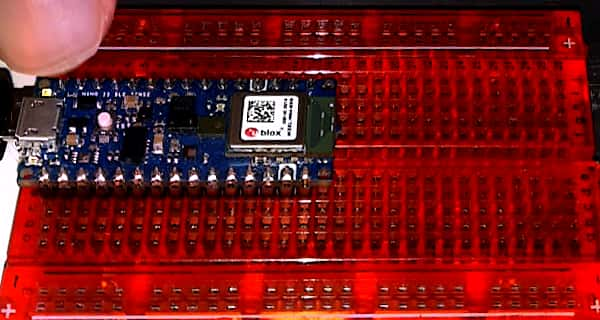
\includegraphics[width=1.0\linewidth]{Nano33BLESense/Click-Reset}
	\caption{Reset Button}
	\label{fig:Check-Reset}
\end{figure}

By clicking the white reset button, the arduino borad will be in boot setup and make sure to check the orange LED glow as shown in the figure \ref{fig:LED-Glow}.

\begin{figure}[h]
	\centering
	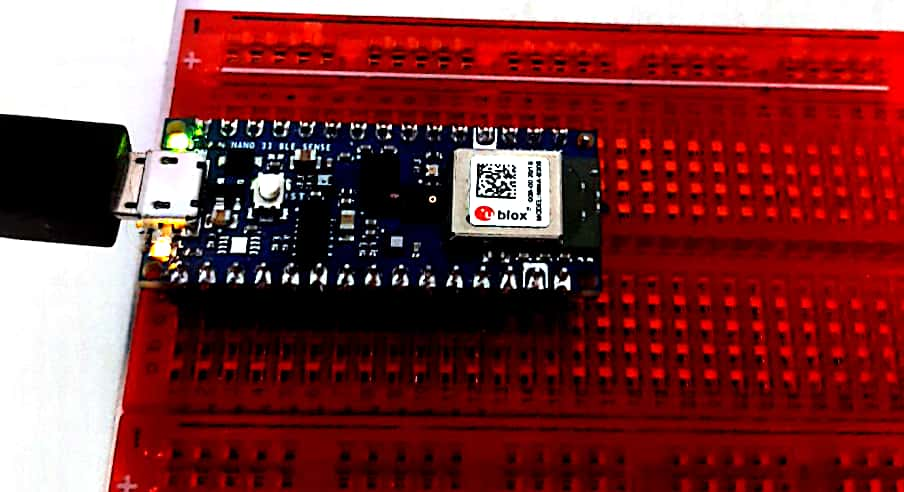
\includegraphics[width=1.0\linewidth]{Nano33BLESense/Orange LED}
	\caption{Orange LED Glow}
	\label{fig:LED-Glow}
\end{figure}

After successfully applying the above mention step, next we need to select the connected port before upload the program. For this, go to tool select arduino port and make sure to check it available port for uploading the program as shown in figure \ref{fig:Port-Selection}

\begin{figure}[h]
	\centering
	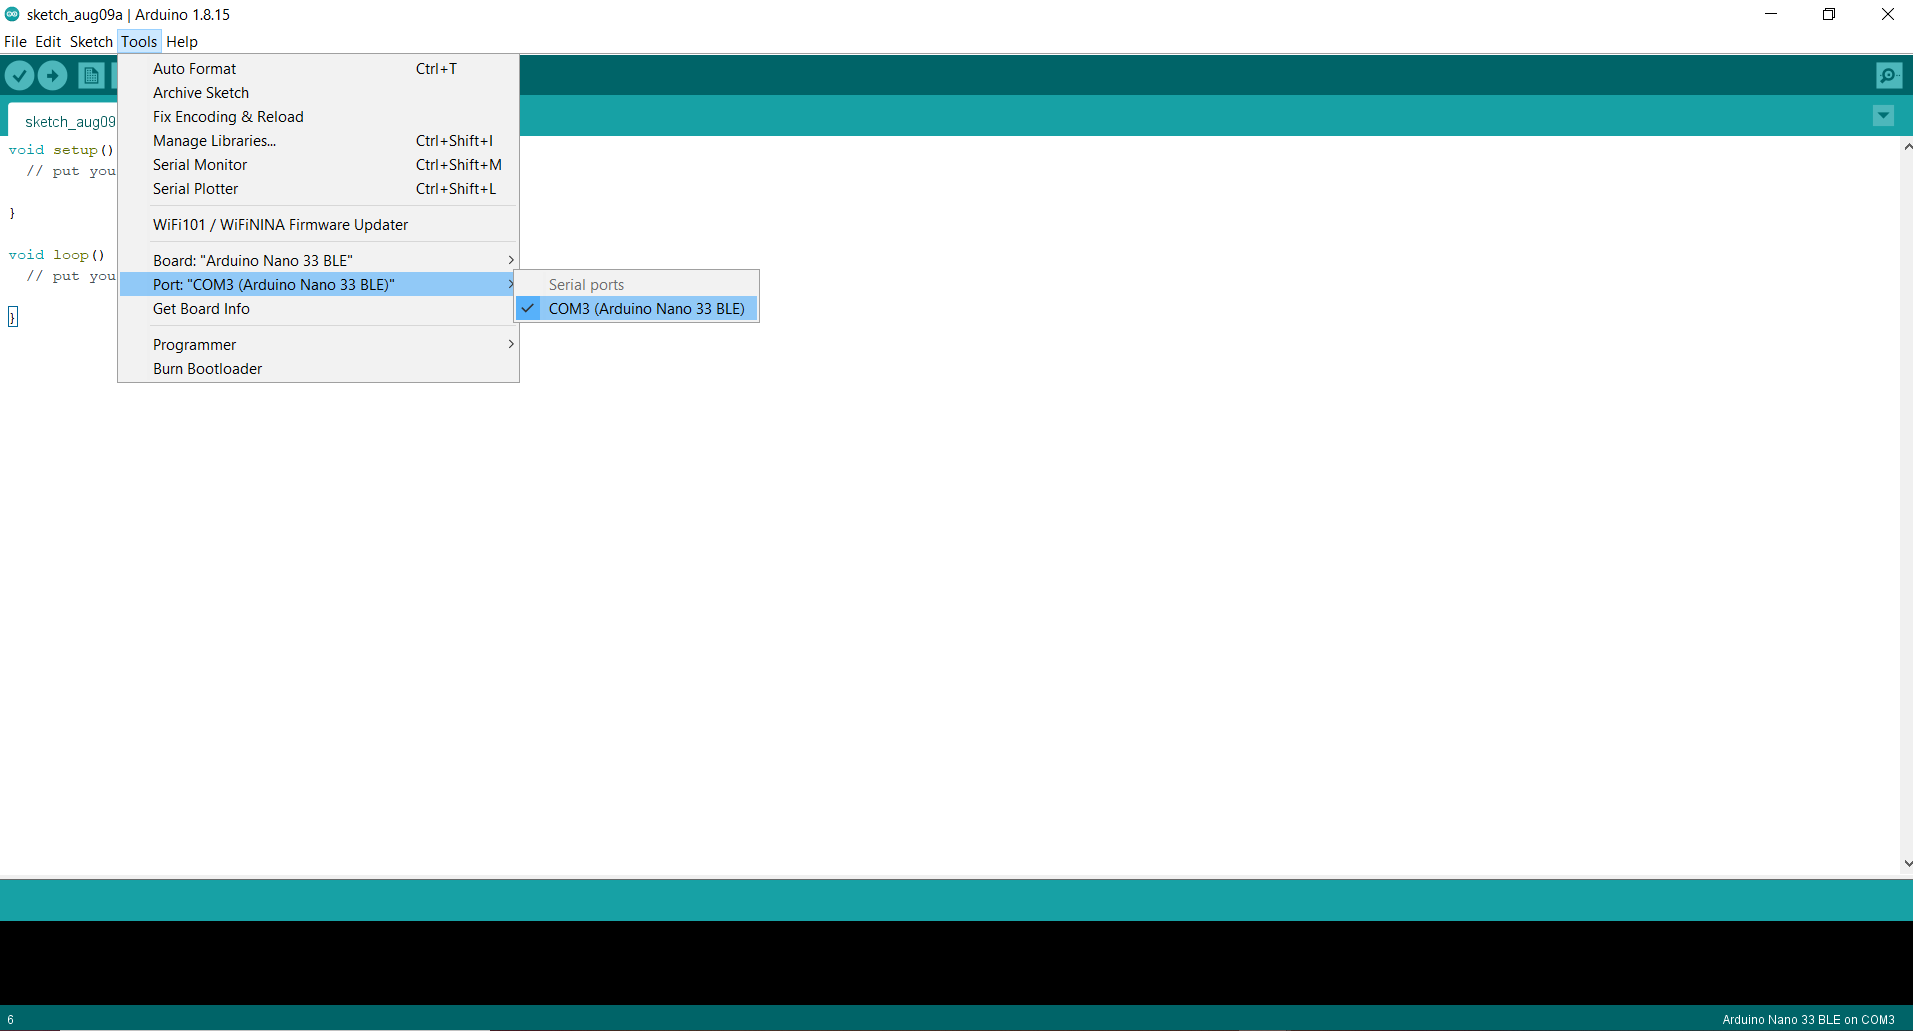
\includegraphics[width=1.0\linewidth]{Nano33BLESense/Port-Select}
	\caption{Select Available Port for Uploading Arduino Sketch}
	\label{fig:Port-Selection}
\end{figure}

\subsection{Upload Code in Arduino Board}

By making sure to select the appropriate port, it's time to upload the Arduino program. There are five icons (verify, upload, new, open, save) below the file section, before uploading the program the best practice is to verify the program first, it show us if there are any error or warning in the program exist or not. By successfully verifying the program we can safely upload the program by click the upload button in the top below the file section as shown in figure. \ref{fig:Upload}.


\begin{figure}[h]
	\centering
	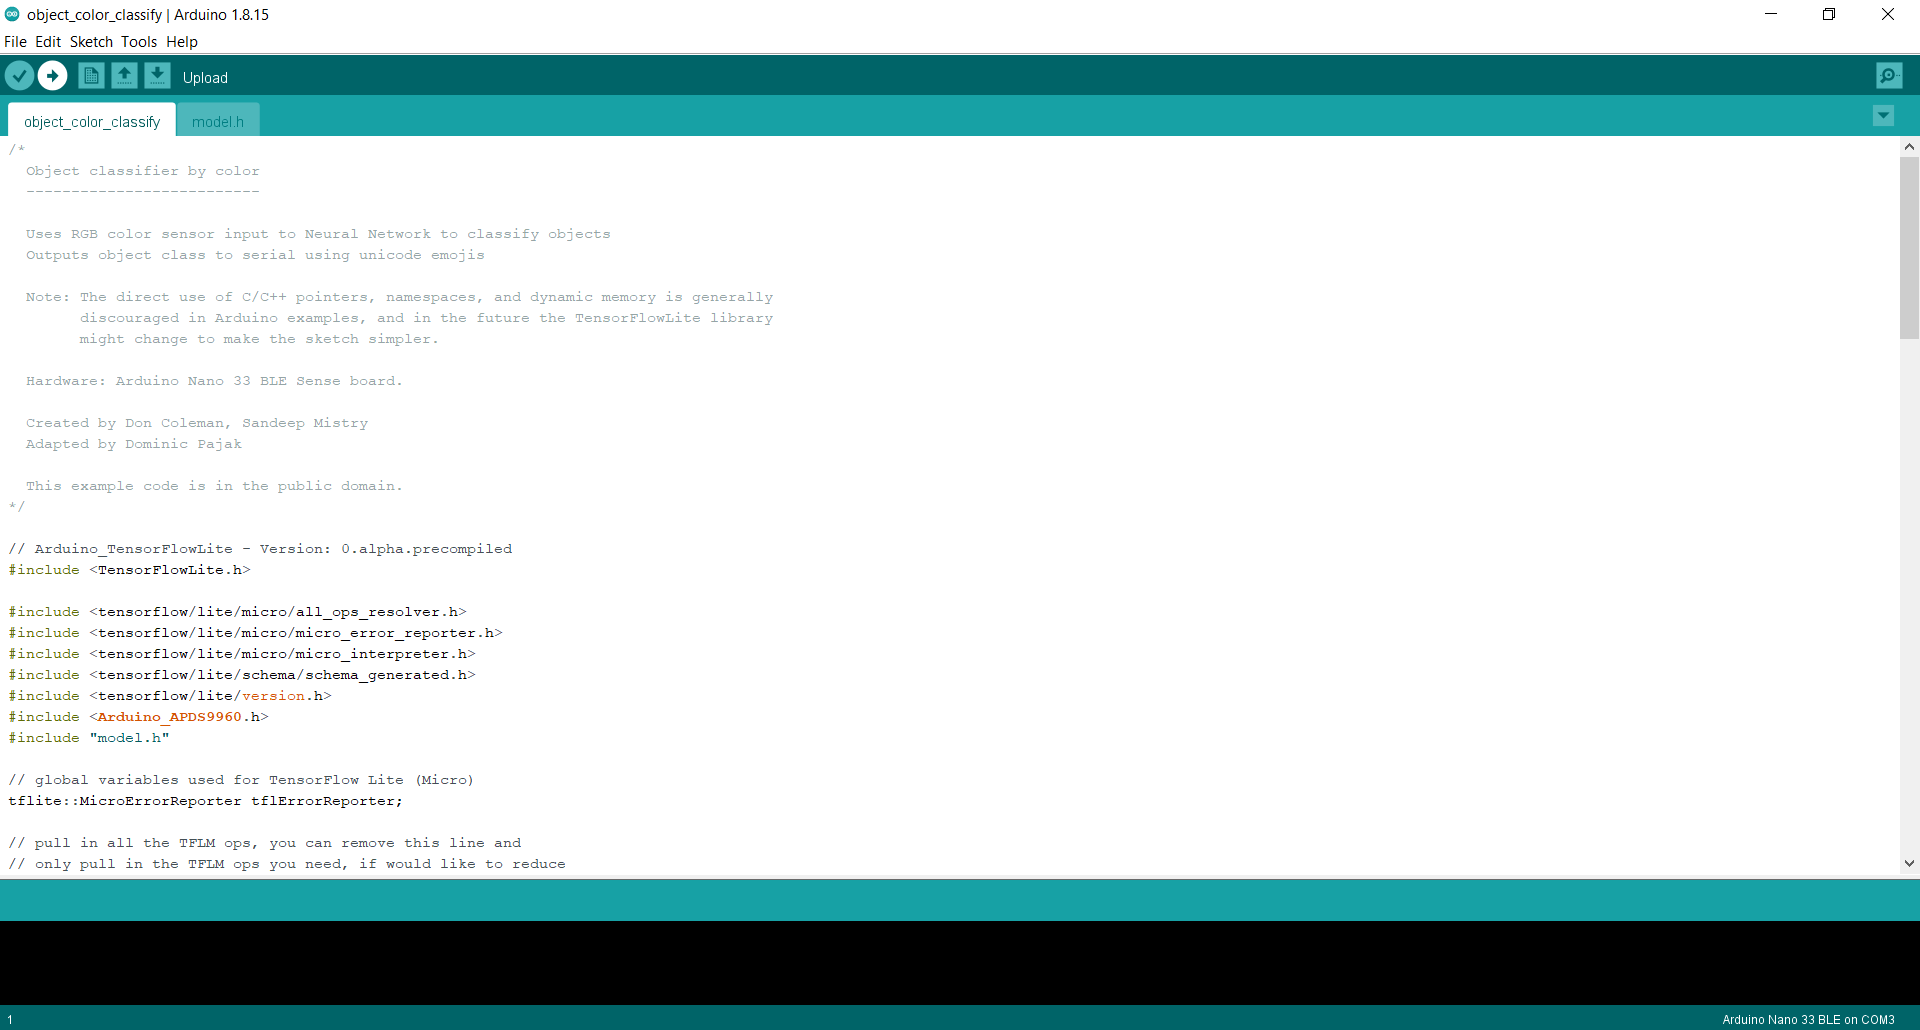
\includegraphics[width=1.0\linewidth]{Nano33BLESense/Upload}
	\caption{Upload the Program in Arduino board}
	\label{fig:Upload}
\end{figure}

After uploading, the code will compile and if there is any issue in our program it will pop up in the bottom black window as well.

After successfully uploading and compiling the code in Arduino board, it also require to change the port again as we did it previously. Go to tool select arduino port and make sure to check the port again as shown in figure \ref{fig:Port} by getting output in the serial monitor.

\begin{figure}[h]
	\centering
	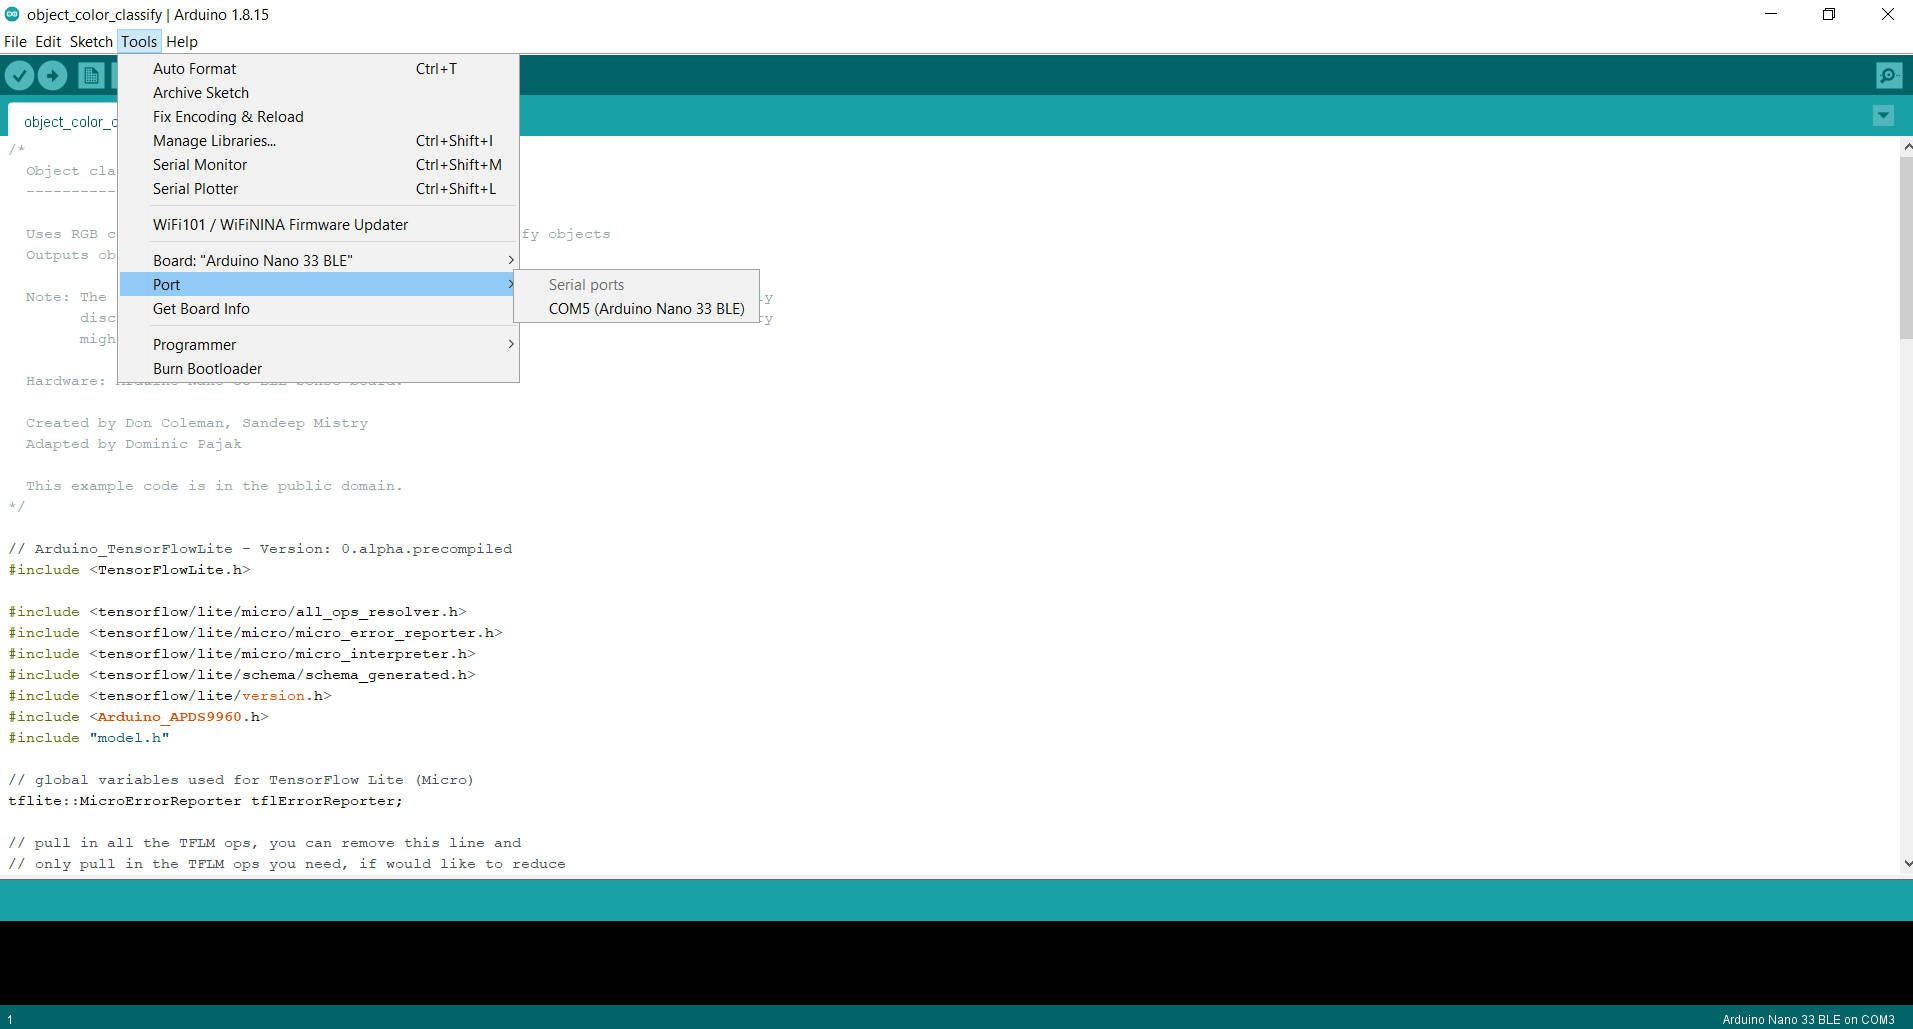
\includegraphics[width=1.0\linewidth]{Nano33BLESense/Port}
	\caption{Setting the Port}
	\label{fig:Port}
\end{figure}

\section{Output Window (Serial Monitor)}

Serial Monitor is the another window on the Arduino IDE, which shows the Input/Output of our program and results appear on it as per the required output. For getting access to Serial monitor, we need to go extreme right in the Arduino IDE, the small circle pop up when we reach it is the serial monitor as show in the figure. \ref{fig:Serial Monitor}

\begin{figure}[h]
	\centering
	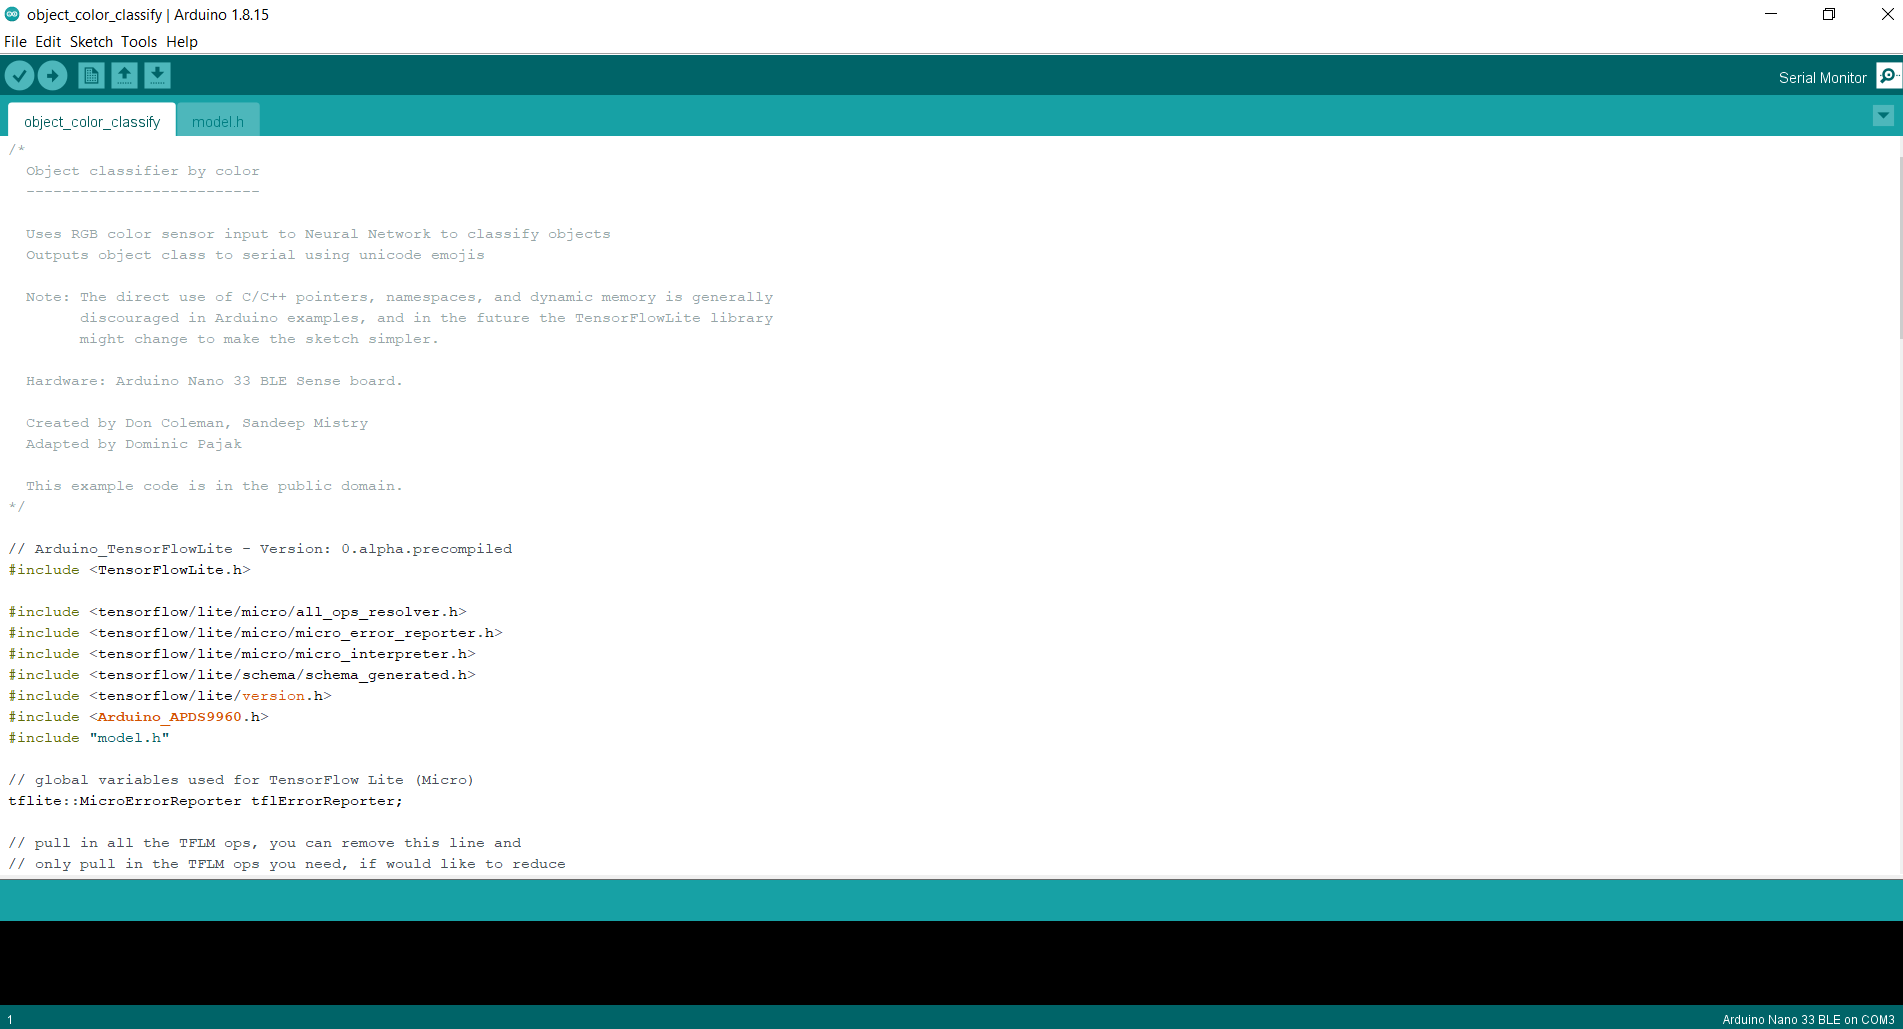
\includegraphics[width=1.0\linewidth]{Nano33BLESense/Serial Monitor}
	\caption{Serial Monitor Icon}
	\label{fig:Serial Monitor}
\end{figure}

The Final results, all the variables, input, sensor values are shown in the serial monitor the (Output Window)  as shown in the figure \ref{fig:Output Window} by clicking the serial monitor button.

\begin{figure}[h]
	\centering
	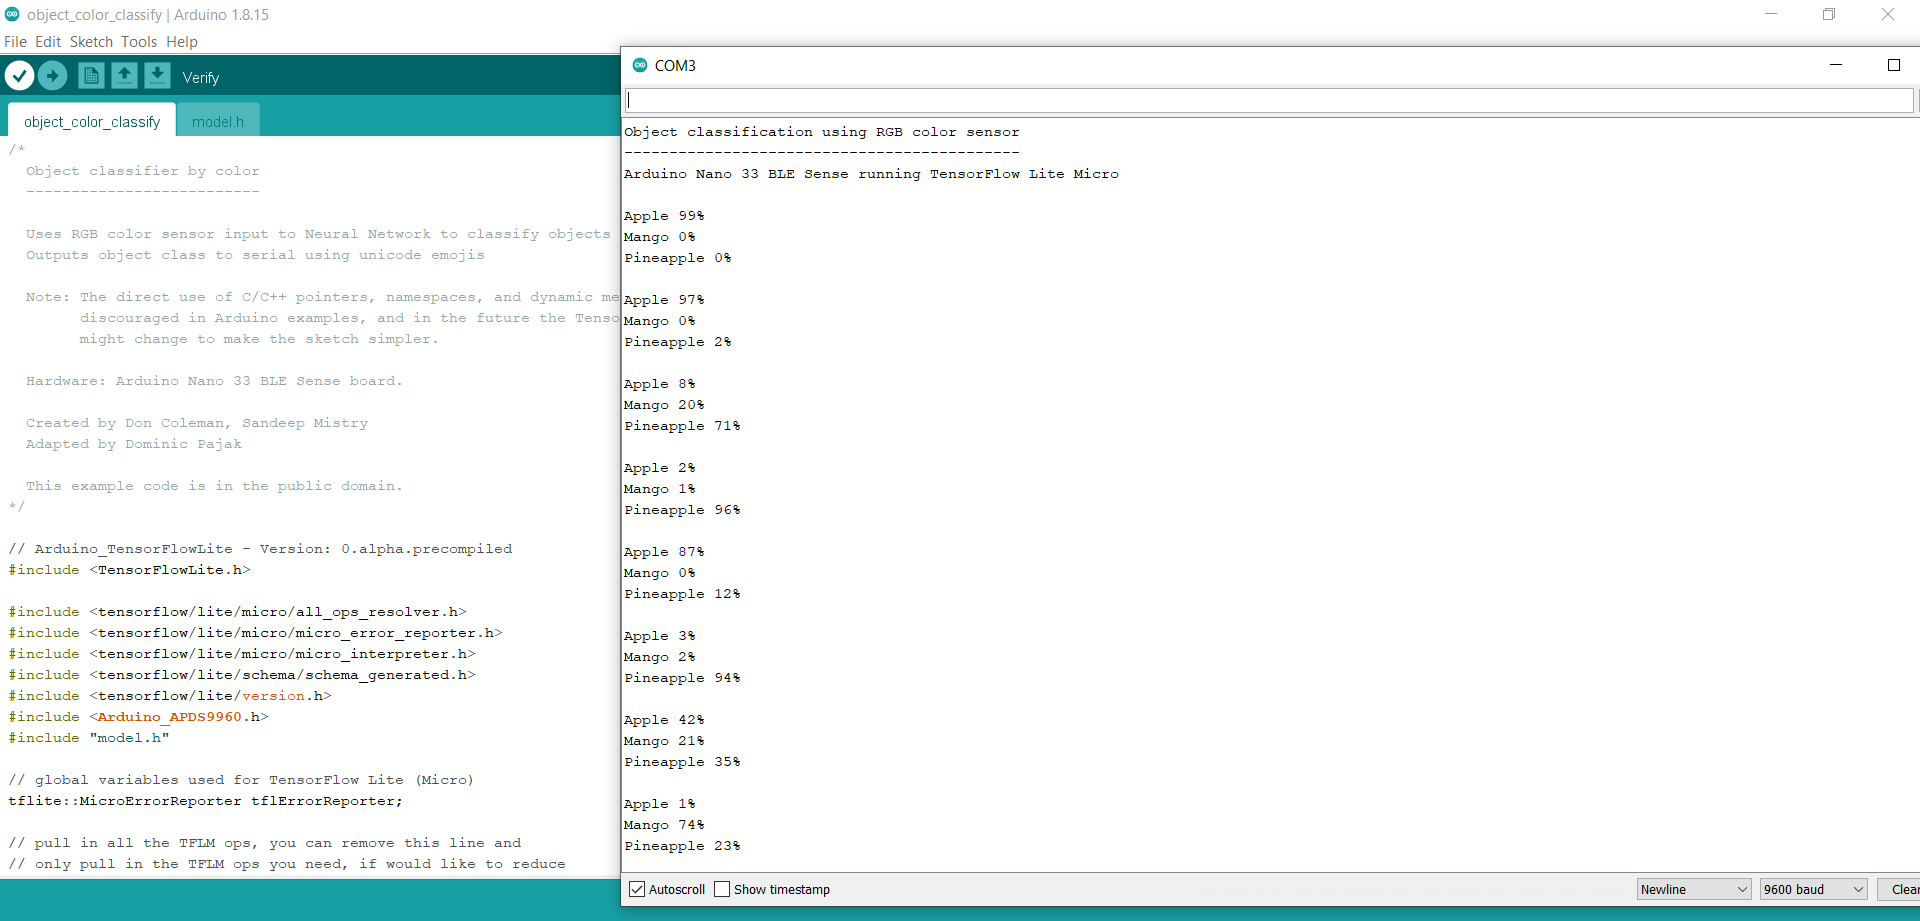
\includegraphics[width=1.0\linewidth]{Nano33BLESense/4}
	\caption{Output Window}
	\label{fig:Output Window}
\end{figure}

\section{Python on Pycharm}

PyCharm is an integrated development environment (IDE) from the JetBrains company for the Python programming language. This Integrated development environment offers only the python programming environment, which will be usefull later in our project for running some computer vision python module.


\subsection{Pycharm Installation}

For getting up to date latest version of pycharm, we need to go \href{https://www.jetbrains.com/pycharm/download/#section=windows}{JetBrains-Link} and install the appropriate version as per our Operating system. 

\section{Python Installation}

Python is commonly used for developing websites and software, task automation, data analysis, and data visualization. Since it's relatively easy to learn, Python has been adopted by many non-programmers such as accountants and Data scientists, for a variety of everyday tasks, like organizing finances. It is an interpreted, object-oriented, high-level programming language with dynamic semantics. \href{https://www.python.org/downloads/}{Python Installation} at the time of writing this report the latest version of python is 3.9.7 release.\ref{Python Installation}

\begin{figure}[h]
	\centering
	\includegraphics[width=1.0\linewidth]{Nano33BLESense/python}
	\caption{Python Installation}
	\label{Python Installation}
\end{figure}

\section{Anaconda supporting framework for Jupyter Notebook}

Anaconda is a distribution of the Python and R programming languages for scientific computing (data science, machine learning applications, large-scale data processing, predictive analytics, etc.), that aims to simplify package management and deployment. It is the most popular toolkit for data science environment. It support every package of Machine learning and Artificial Intelligence. The most widely used packages in machine learning are TensorFlow, OpenCV, and MediaPipe. the other supporting libraries include Numpy, Pandas, Matplotlib, Sklearn and many more. For getting up to date documentation and installation guide available at \href{https://www.anaconda.com/products/individual}{Jupyter notebook}. Anaconda support Jupyter notebook web application, it is the most widely used notebook for writing and training the Machine learning models.


\chapter{Test}

\section{General Tests}

All the Arduino boards need power to operate, either it comes from the USB connection with Laptop, Ac power adapter, Battery or a regulated power supply. The most easiest way to operate arduino board is USB connection with laptop, normally these boards need 5V direct current (DC) to operate. Arduino Nano 33 BLE sense also need these types of power sources for funcnality, when applying one of the above mention power source the green LED glows as shown in the figure \ref{fig:Test}, it shows the sign of Arduino board working.

\begin{figure}[htbp]
	\centering
	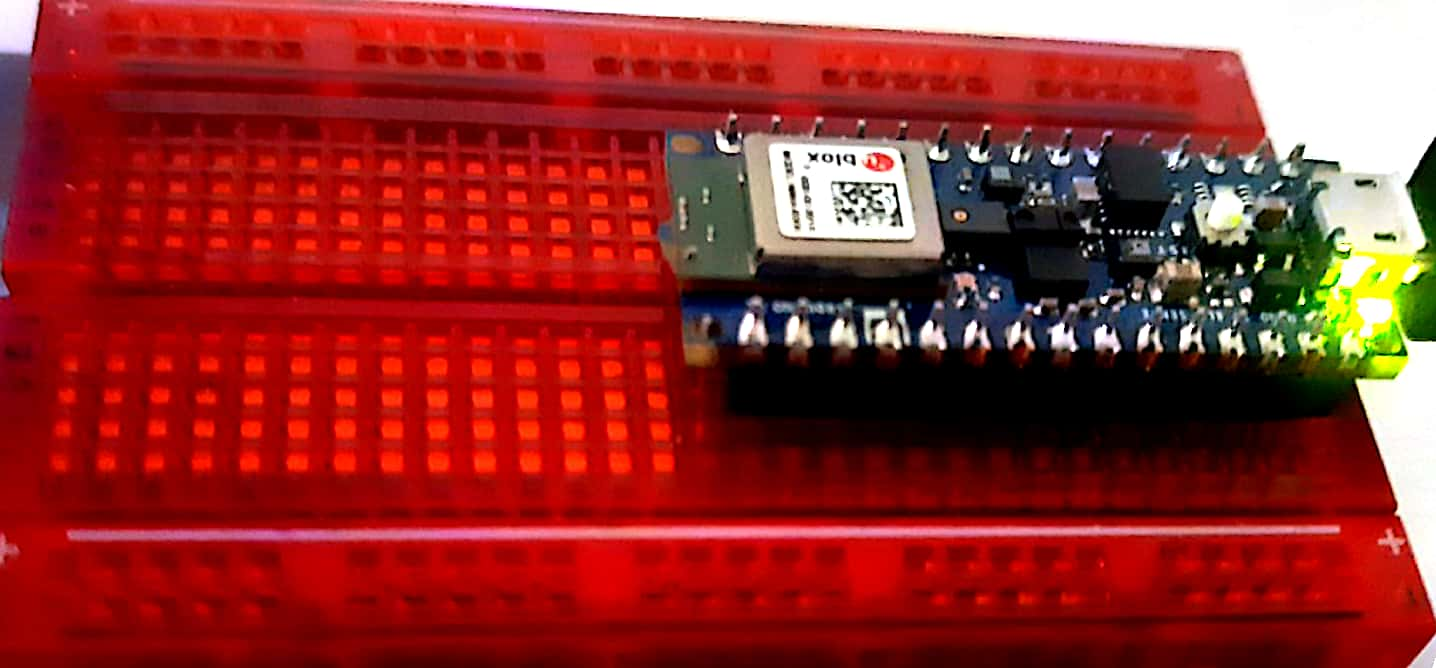
\includegraphics[width=6.5cm]{Nano33BLESense/Test-1}
	\caption{Power On Arduino Nano 33 BLE Sense}
	\label{fig:Test}
\end{figure}

\section{Testing the On-Board Sensor}

Arduino Nano 33 BLE sense have a set of on-board sensor embed on it. These sensor also start working when arduino board operate. These are the following set of sensors available in Arduino Nano 33 BLE Sense board.
\begin{itemize}
	\item The IMU is a LSM9DS1 and it is managed through I2C.
	\item The LPS22HB reads barometric pressure and environmental temperature.
	\item The HTS221 senses relative humidity.
	\item The ADPS-9960 is a digital proximity, ambient light, RGB and gesture sensor.
	\item The MP34DT05 is the digital microphone.
\end{itemize} 

\subsection{LSM9DS1 (Accelerometer, Gyroscope, and Magnetometre Sensor)}

The 9-axis inertial measurement unit (IMU) sensor is work as a accelerometre, gyroscope, and magnetic sensor. It measures 3D linear acceleration, 3D angular Velocity and 3D magnetic field aroud the sensor. This 9-axis IMU sensor use to measure Position, vibration, orientation and magnetic field around the sensor. To check the funcnality of this sensor there is avialable library in the example section as shown in the figure. \ref{fig:Testware} Go to examples check LSM9DS1 sensor, it shows all the functionality of this sensor i.e: (Accelerometer, Gyroscope, and Magnetometer).


\begin{figure}[htbp]
	\centering
	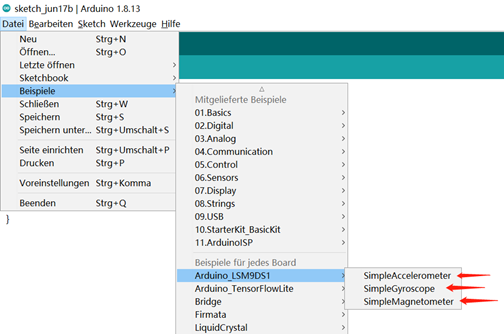
\includegraphics[width=7.5cm]{Nano33BLESense/Testware3Sensoren}
	\caption{9-Axis IMU Sensor}
	\label{fig:Testware}
\end{figure}

By getting the results and output of the 9-axis IMU sensor, first we need to upload the available library program into Arduino nano 33 BLE Sense. To avoid any trouble during uploading the program, make sure to follow all the steps as we discussed in previous chapter e.g; (choose the board, select the port during upload and change the port when need to see output in serial monitor, reset arduino when needed). By uploading the program successfully, open the serial monitor and see the result as shown in figure.\ref{fig:IMU-Test} Make sure to change the position and orientation of board and also place some Magnet aroud the borad, it shows visible changes in the output too.

\begin{figure}[htbp]
	\centering
	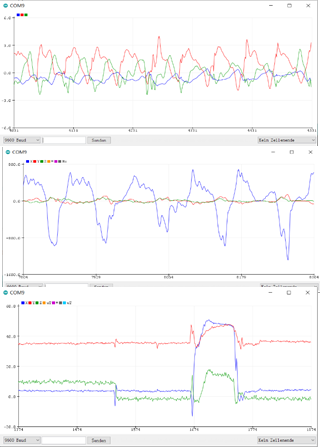
\includegraphics[width=7.5cm]{Nano33BLESense/ErgebnisseIMUTests}
	\caption{Results of IMU-Tests}
	\label{fig:IMU-Test}
\end{figure}

The above 9-Axis IMU output, shows the 3-axis values for each accelerometer, gyroscope and magnetometer. It shows how powerful the Arduino Nano 33 ble sense board and compatible with Arduino IDE the integrated development environment. These values changes as the sensor observes some changing in the sorroundings too, and it shows in the form of graph in the serial monitor. 


\subsection{APDS-9960 (Gesture, Proximity, and Color Detection Sensor)}
APDS-9960 sensor has the funcnality of proximity distance measure, RGB color detection, and Gesture detection too. It is also on-board embed sensor on Arduino nano 33 BLE Sense and has the same procedure for uploading and compiling the program as the 9-axis IMU sensor has. Go to example, check the APDS-9960 library and upload the complete program as shown in the figure. \ref{fig:1} Full example includes the RGB color detection code, gesture detection code, and also proximity distance measure code.

\begin{figure}[htbp]
	\centering
	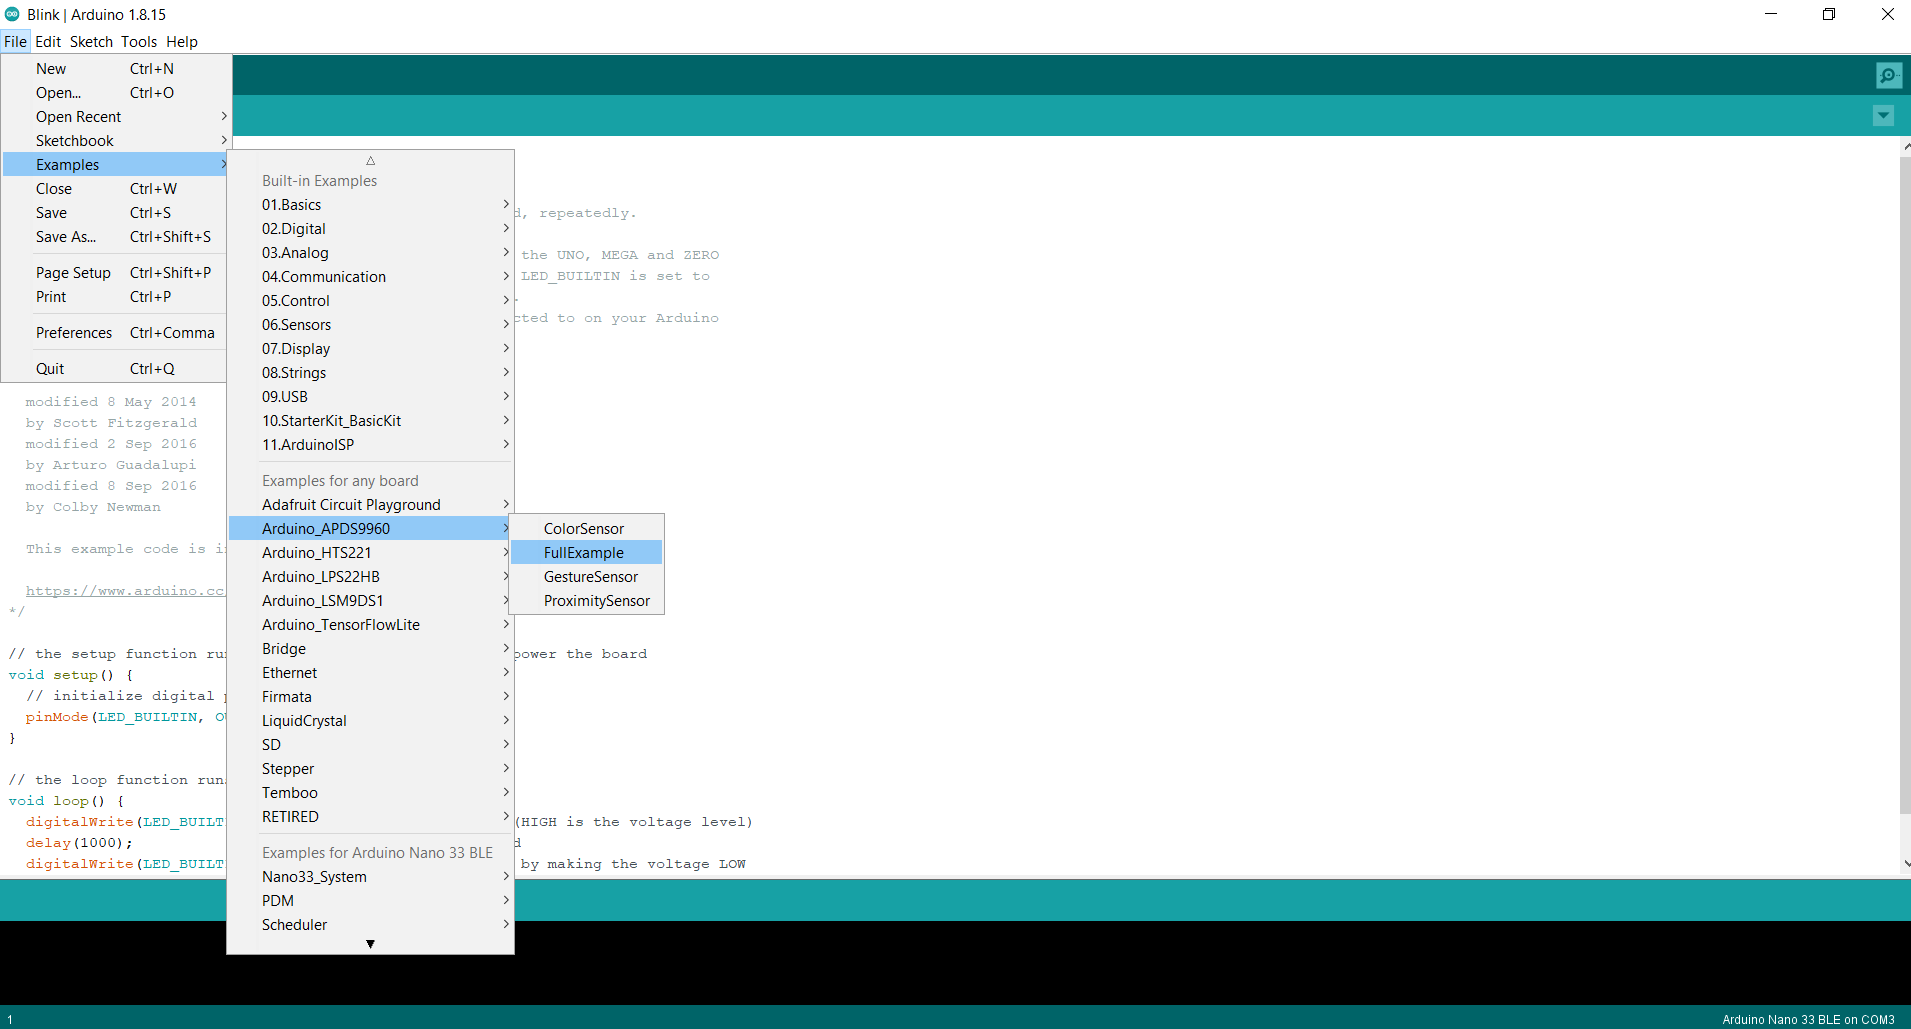
\includegraphics[width=7.5cm]{Nano33BLESense/APDS}
	\caption{APDS-9960 Gesture, Proximity, Color Sensor}
	\label{fig:1}
\end{figure}

Similarly, by following all the steps for uploading and compiling the program we can see the results of APDS-9960 Sensor on serial monitor too. For seeing the different output, we can change the input for the sensor too, e.g: for color detection we can switch the colors, for gesture detection we can also switch the gestures, and for proximity also do the same. The resulted output as shown in the figure.  \ref{fig:2} 

\begin{figure}[htbp]
	\centering
	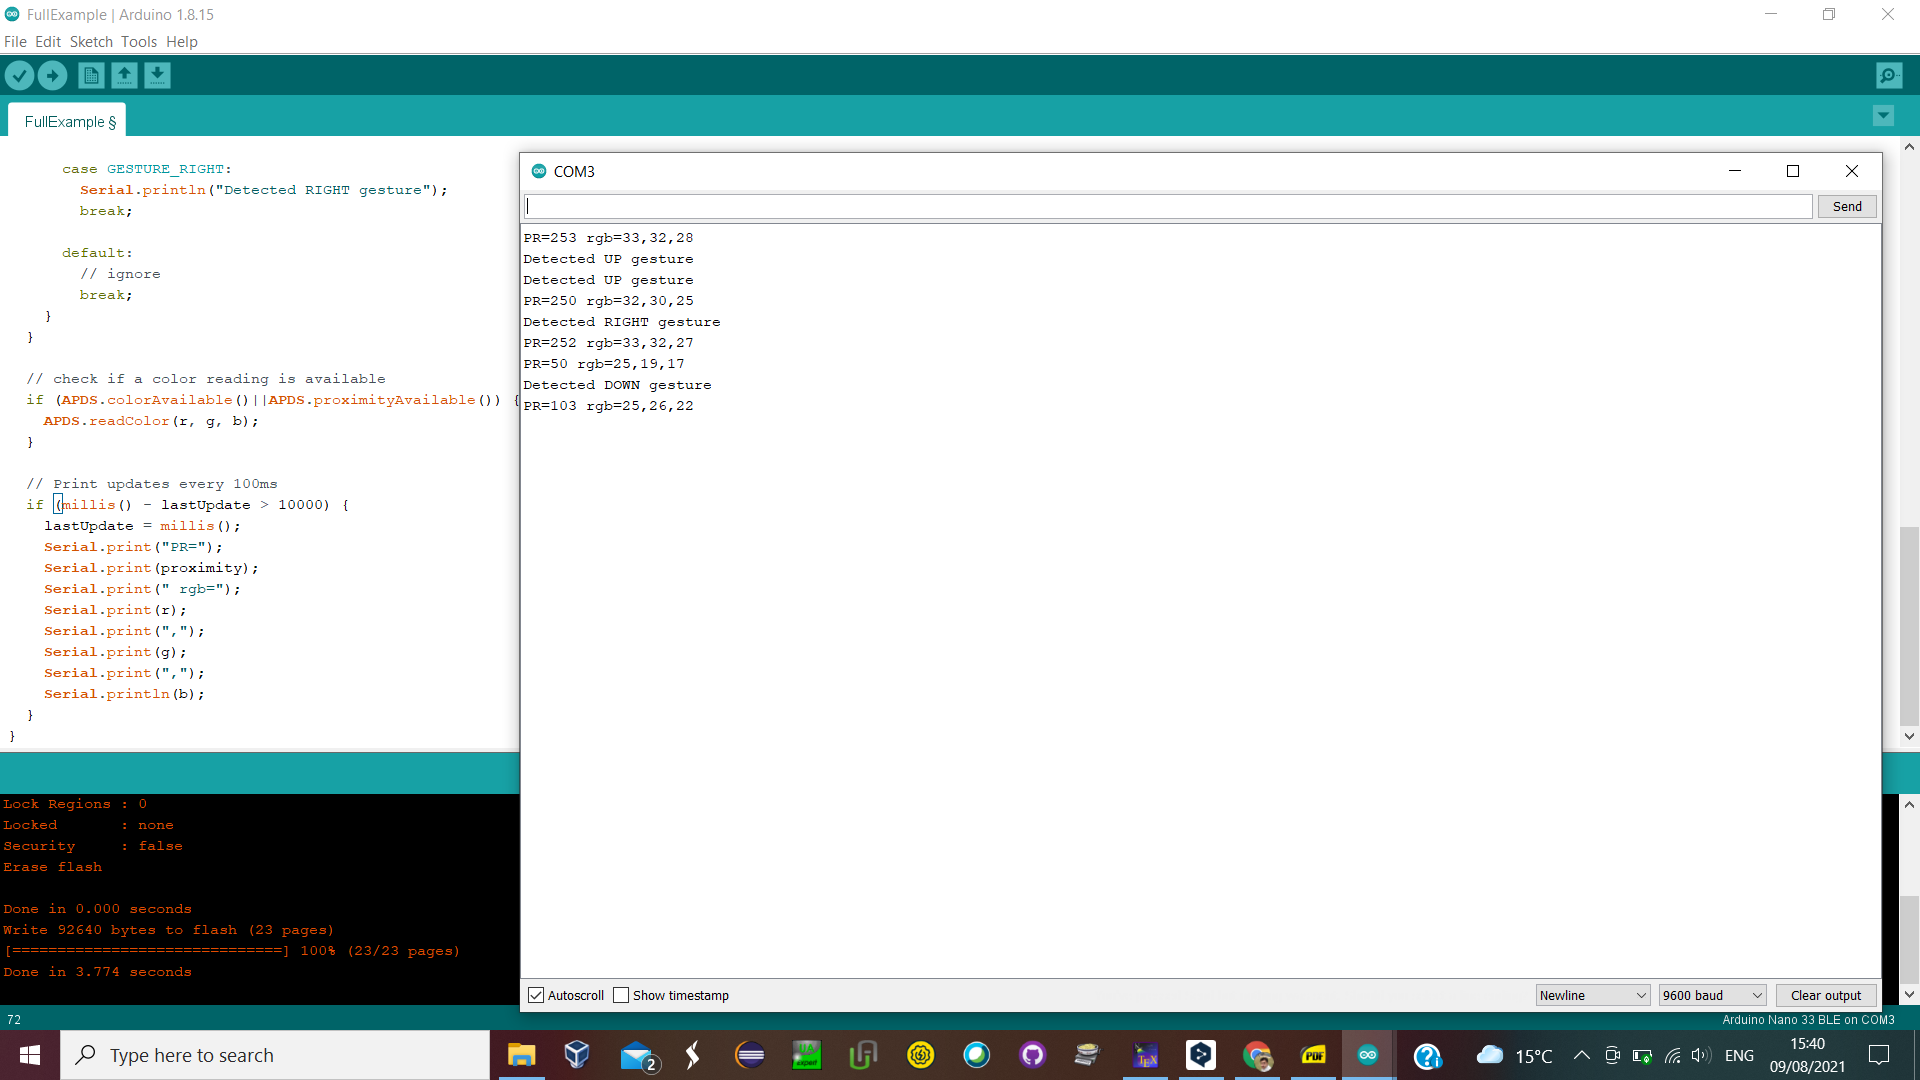
\includegraphics[width=9.5cm]{Nano33BLESense/APDS-Output}
	\caption{Gesture, Proximity, Color Sensor Output Window}
	\label{fig:2}
\end{figure}

We can also run the single funcnality of this sensor too, e.g; if we just need to capture the color of product, we can also run the color detection program. It depends upon the application and we can implement our application and modify the code as per our desire results.

\subsection{LPS22HB (Pressure Sensor)}
Arduino Nano 33 BLE sense also capable of measuring environmental or ambient pressure with the help of LPS22HB on-board embed sensor on it. There is also available library program in Arduino IDE, we need to install the appropriate library and use it or  modify it as per the required application. The procedure for uploading and compiling the code is same as the above sensors have. By opening the example section from file, then go to LPS22HB and click on read or measuring pressure as shown in the figure.  \ref{fig:3} 

\begin{figure}[htbp]
	\centering
	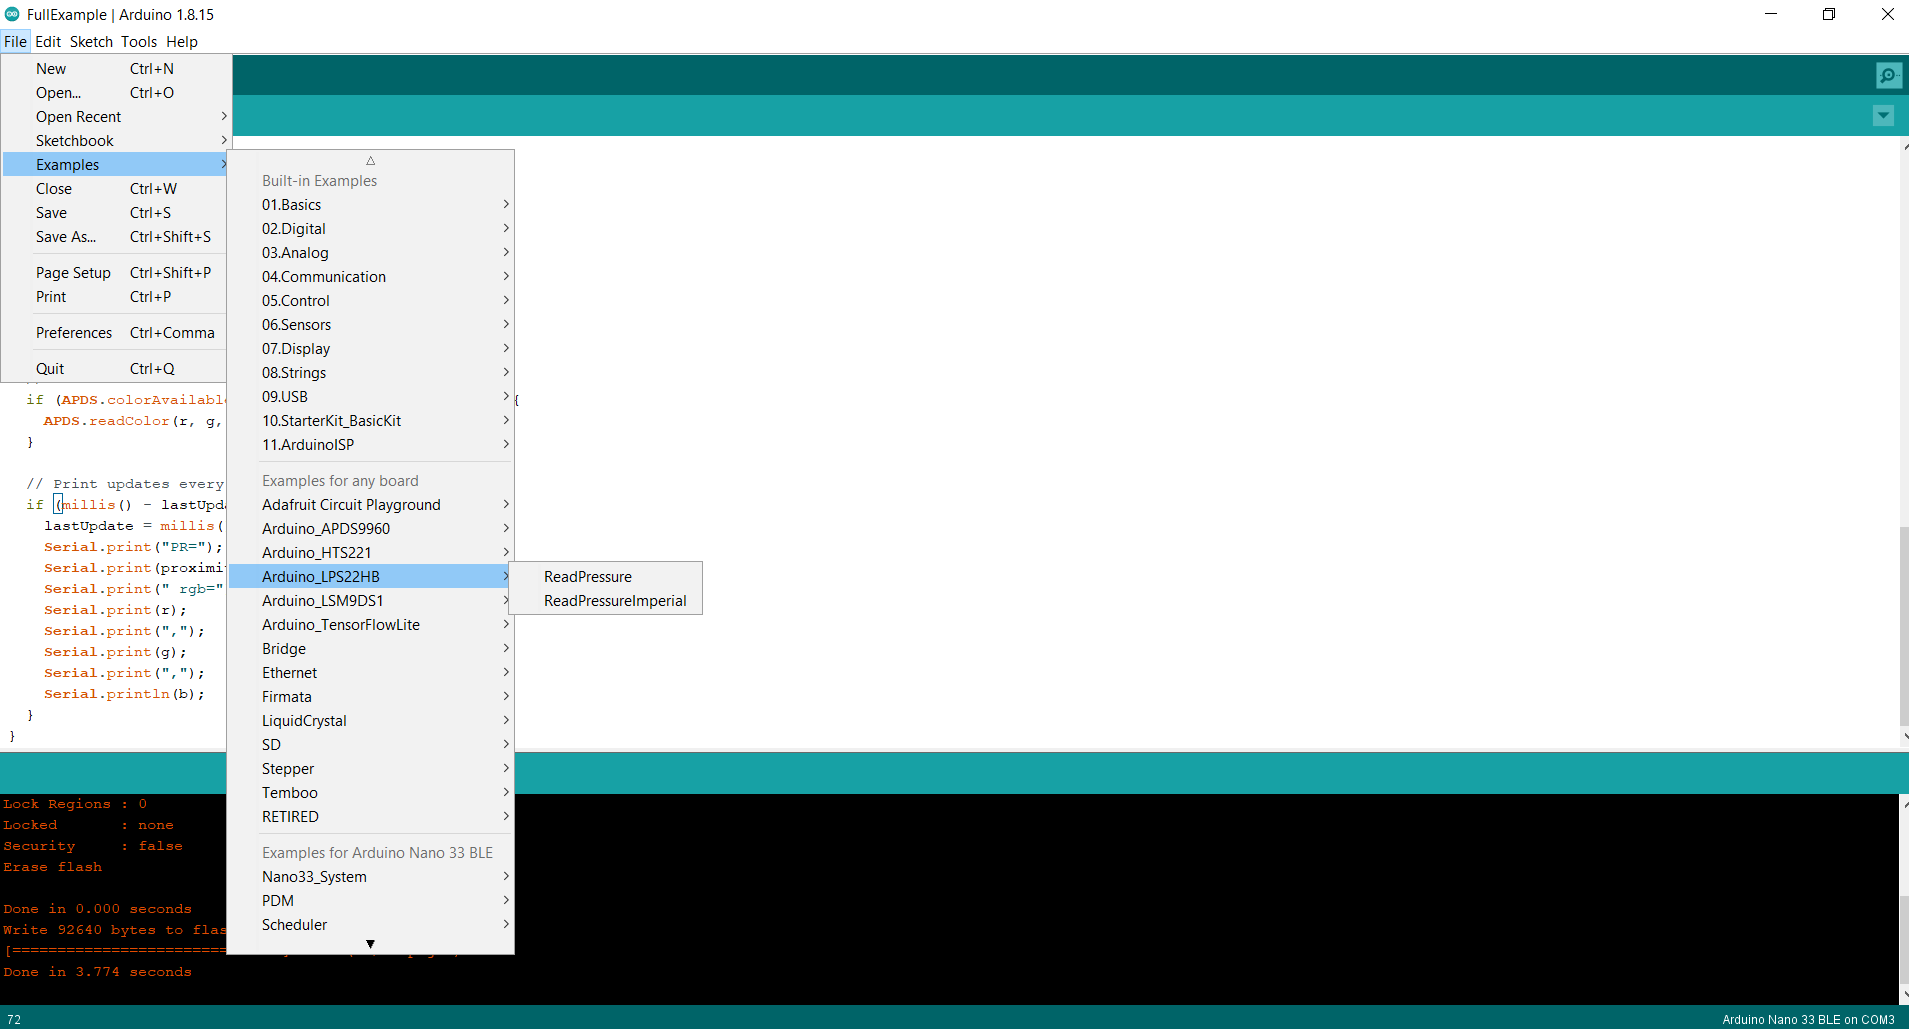
\includegraphics[width=8.5cm]{Nano33BLESense/5}
	\caption{LPS22HB, Pressure and Temperature sensor}
	\label{fig:3}
\end{figure}

The results for LPS22HB the environmental pressure also showed in the serial monitor as shown in the figure.  \ref{fig:4} With the help of these values and modifying the code we can operate some external devices or also just measure the external or internal pressure and apply it wherever it needs.

\begin{figure}[htbp]
	\centering
	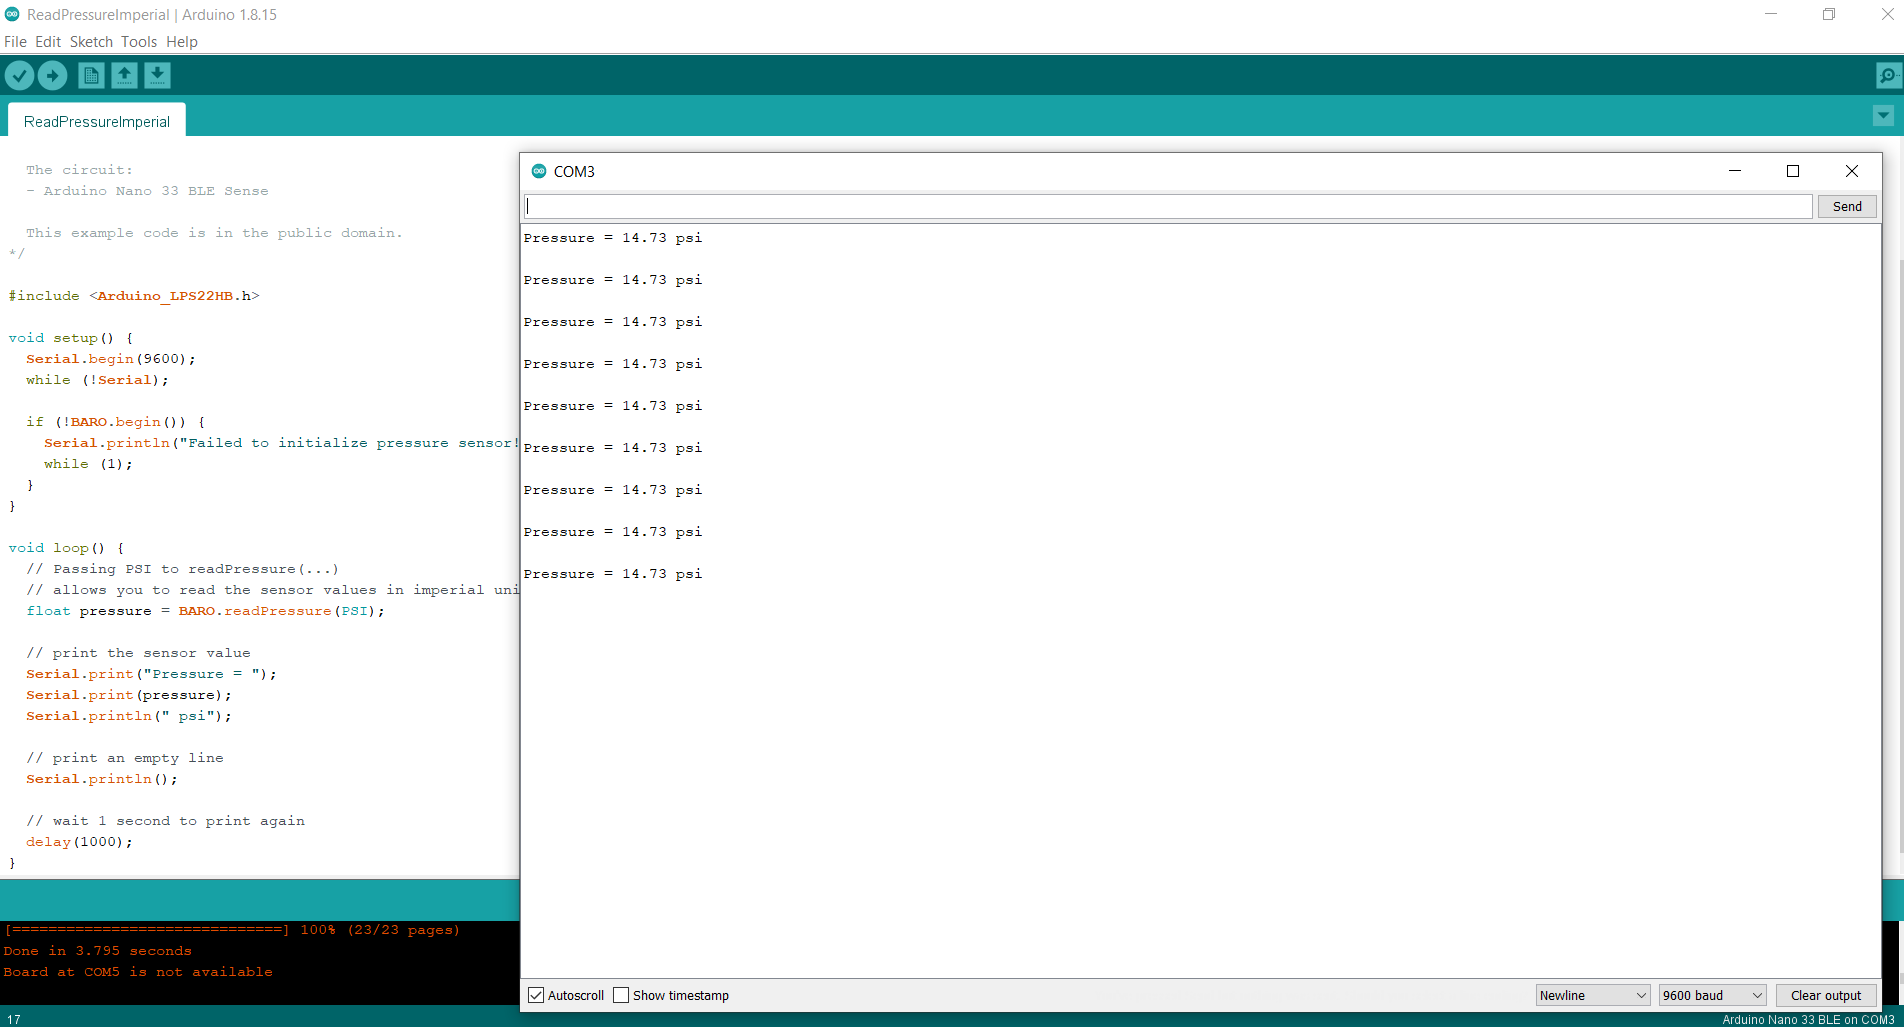
\includegraphics[width=8.5cm]{Nano33BLESense/6}
	\caption{LPS22HB, Output}
	\label{fig:4}
\end{figure}

\subsection{HTS221 (Humidity and Temperature Sensor)}

\begin{figure}[htbp]
	\centering
	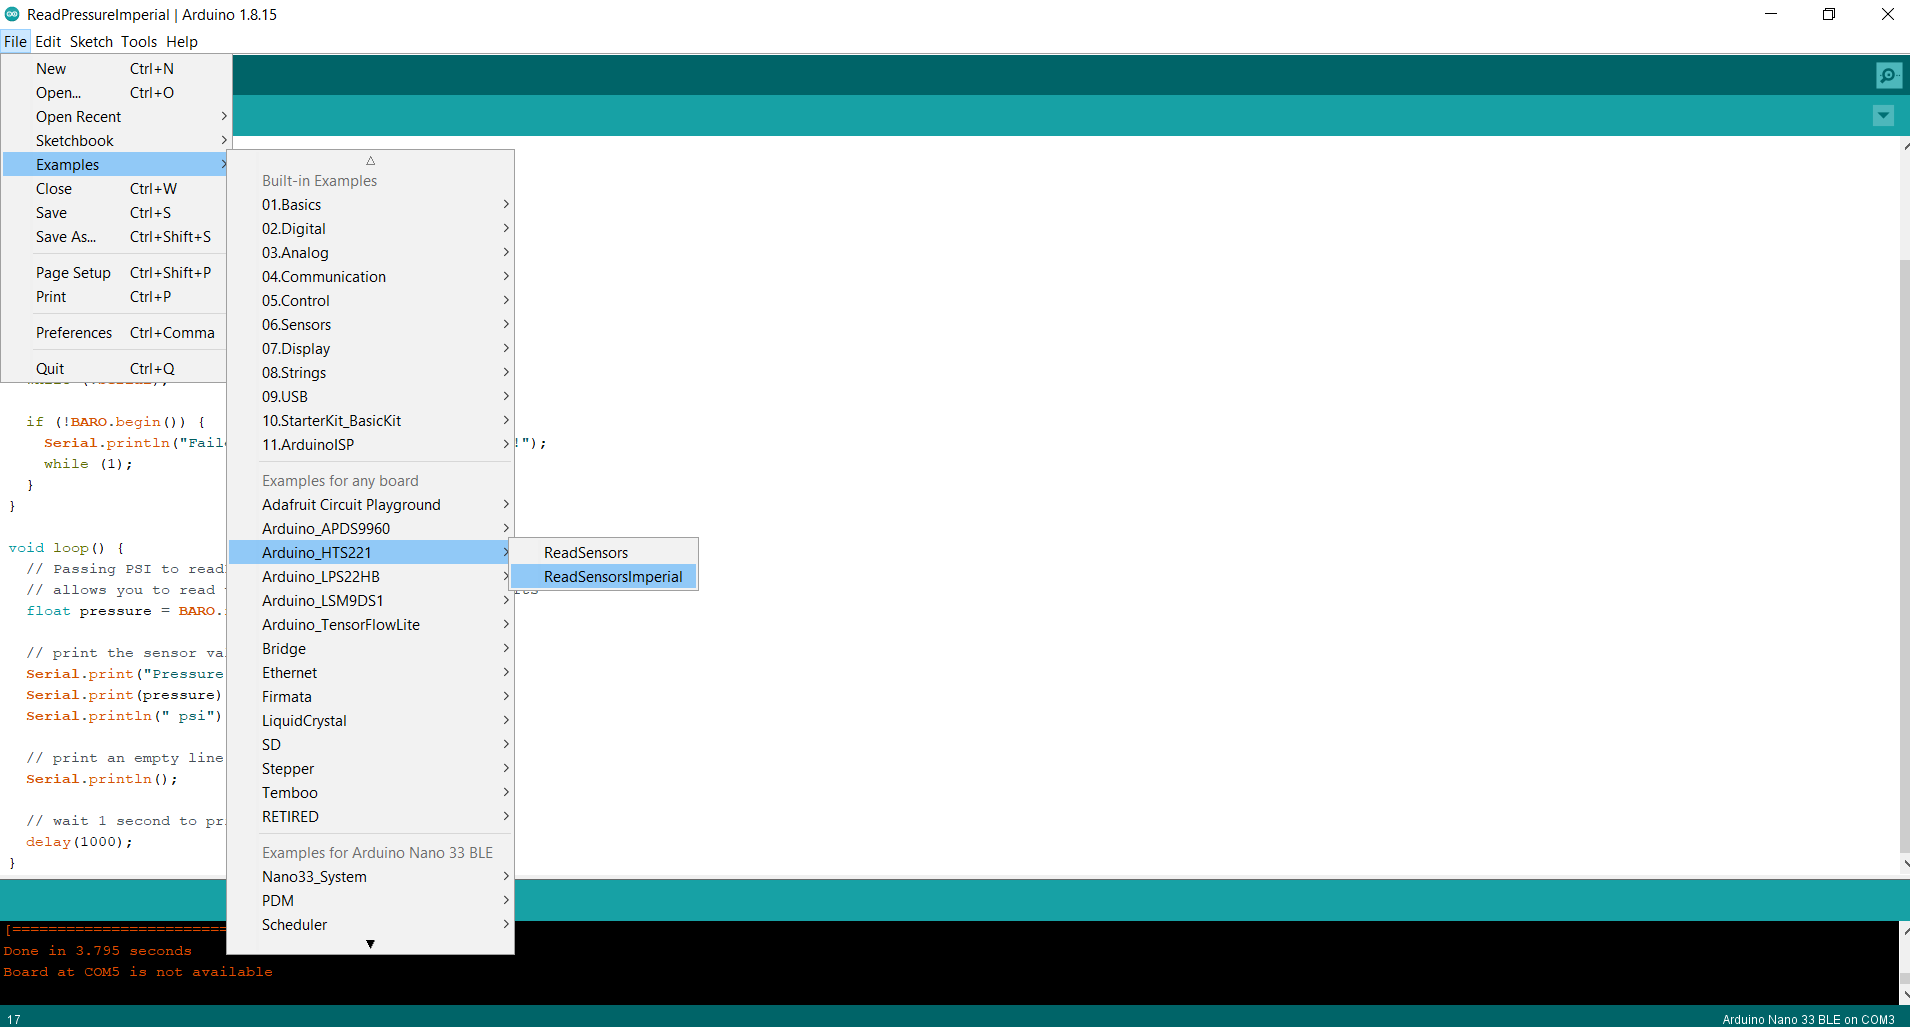
\includegraphics[width=8cm]{Nano33BLESense/7}
	\caption{HTS221, Humidity and Temperature Sensor}
	\label{fig:5}
\end{figure}

The on-board embed HTS221 sensor on Arduino Nano 33 BLE Sense has the funcnality to measure the relative humadity and temperature in the environment. The procedure for getting access to his library and code also the same as the other sensors have as shown in the figure.  \ref{fig:5}

After Uploading and compiling the program, the environmental humidity and temperature also display in the serial monitor as shown in the figure.  \ref{fig:6} By getting access to these values, change the port again after compiling the program for opening the serial monitor, these values help us to make the application with electrical appliances regarding energy savings or modify the code and add some external devices with the GPIO of Arduino Nano 33 BLE Sense too and control it as per the humidity and temperature values.

\begin{figure}[htbp]
	\centering
	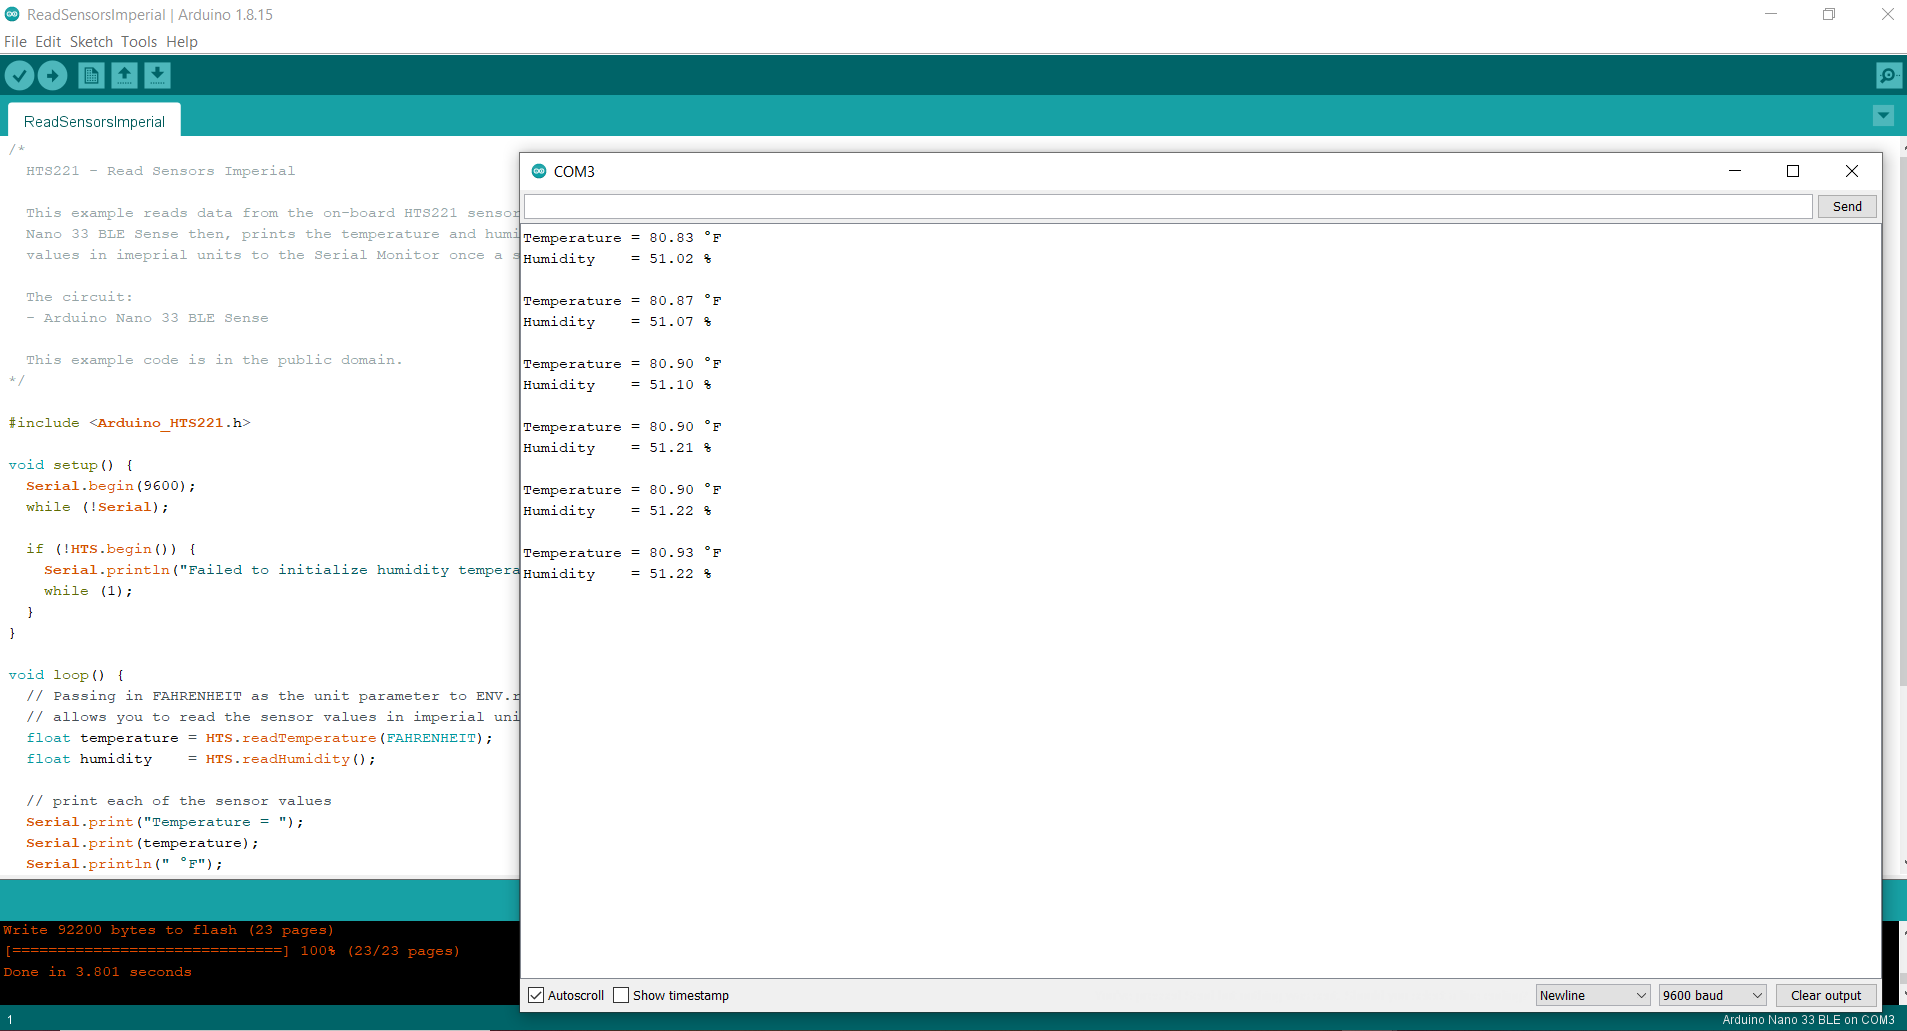
\includegraphics[width=8.5cm]{Nano33BLESense/8}
	\caption{HTS221, Output Window}
	\label{fig:6}
\end{figure}

\subsection{MP34DT05 (Digital Microphone)}

The embed on-board MP34DT05 sensor in Arduino Nano 33 BLE Sense has the funcnality to sense audio voice from the environment. There is build in Arduino library for this particular sensor, which is PDM as shown in the figure.  \ref{fig:7}

\begin{figure}[htbp]
	\centering
	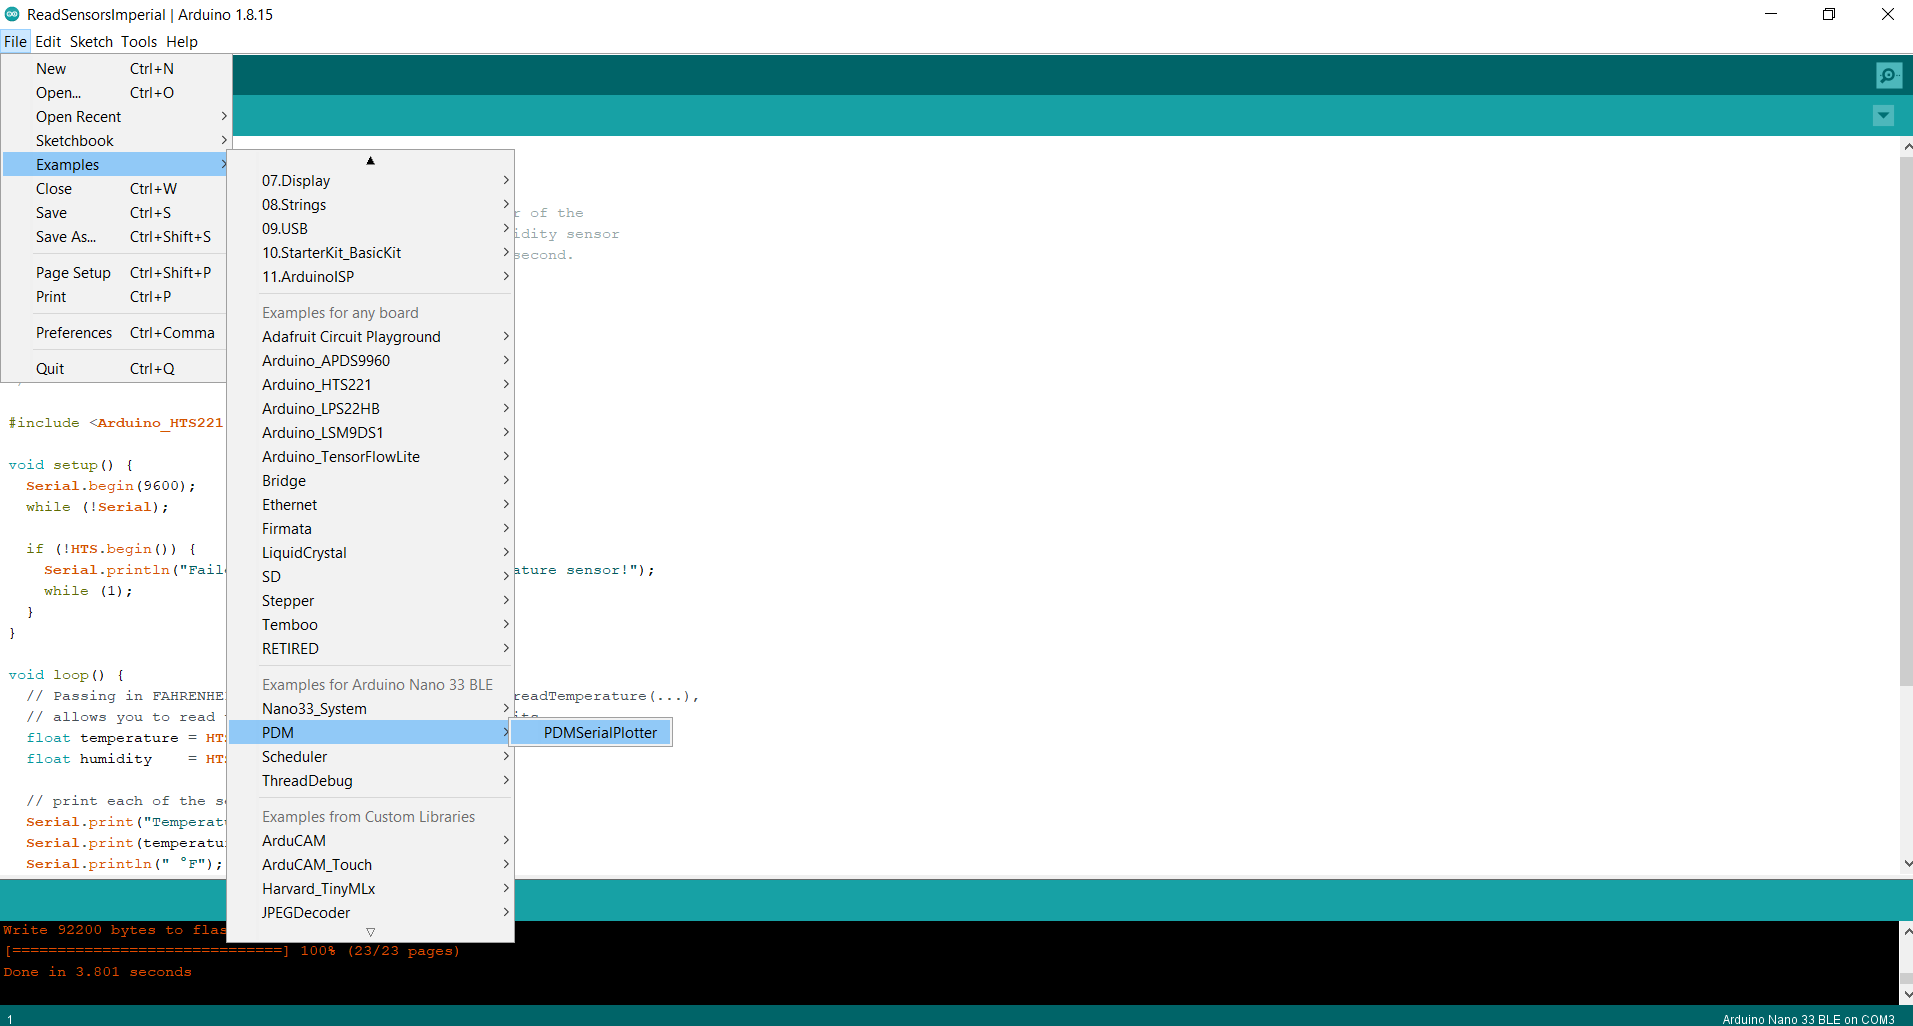
\includegraphics[width=8.5cm]{Nano33BLESense/9}
	\caption{MP34DT05, Digital Microphone}
	\label{fig:7}
\end{figure}

By following the same steps, for this sensor we can see the output the resulted frequency in the serial plotter instaed of serial monitor as shown in figure.  \ref{fig:8}  It is more convenient to understand if we change the loudness of voice the plotter shows us a different frequency curve. MP34DT05 use to detect different voices or words too, with the help of these funcnality we can easily make the valuable application with Arduino Nano 33 BLE Sense by adding some external devices with GPIO pins with the help of 3.3V relay.

\begin{figure}[htbp]
	\centering
	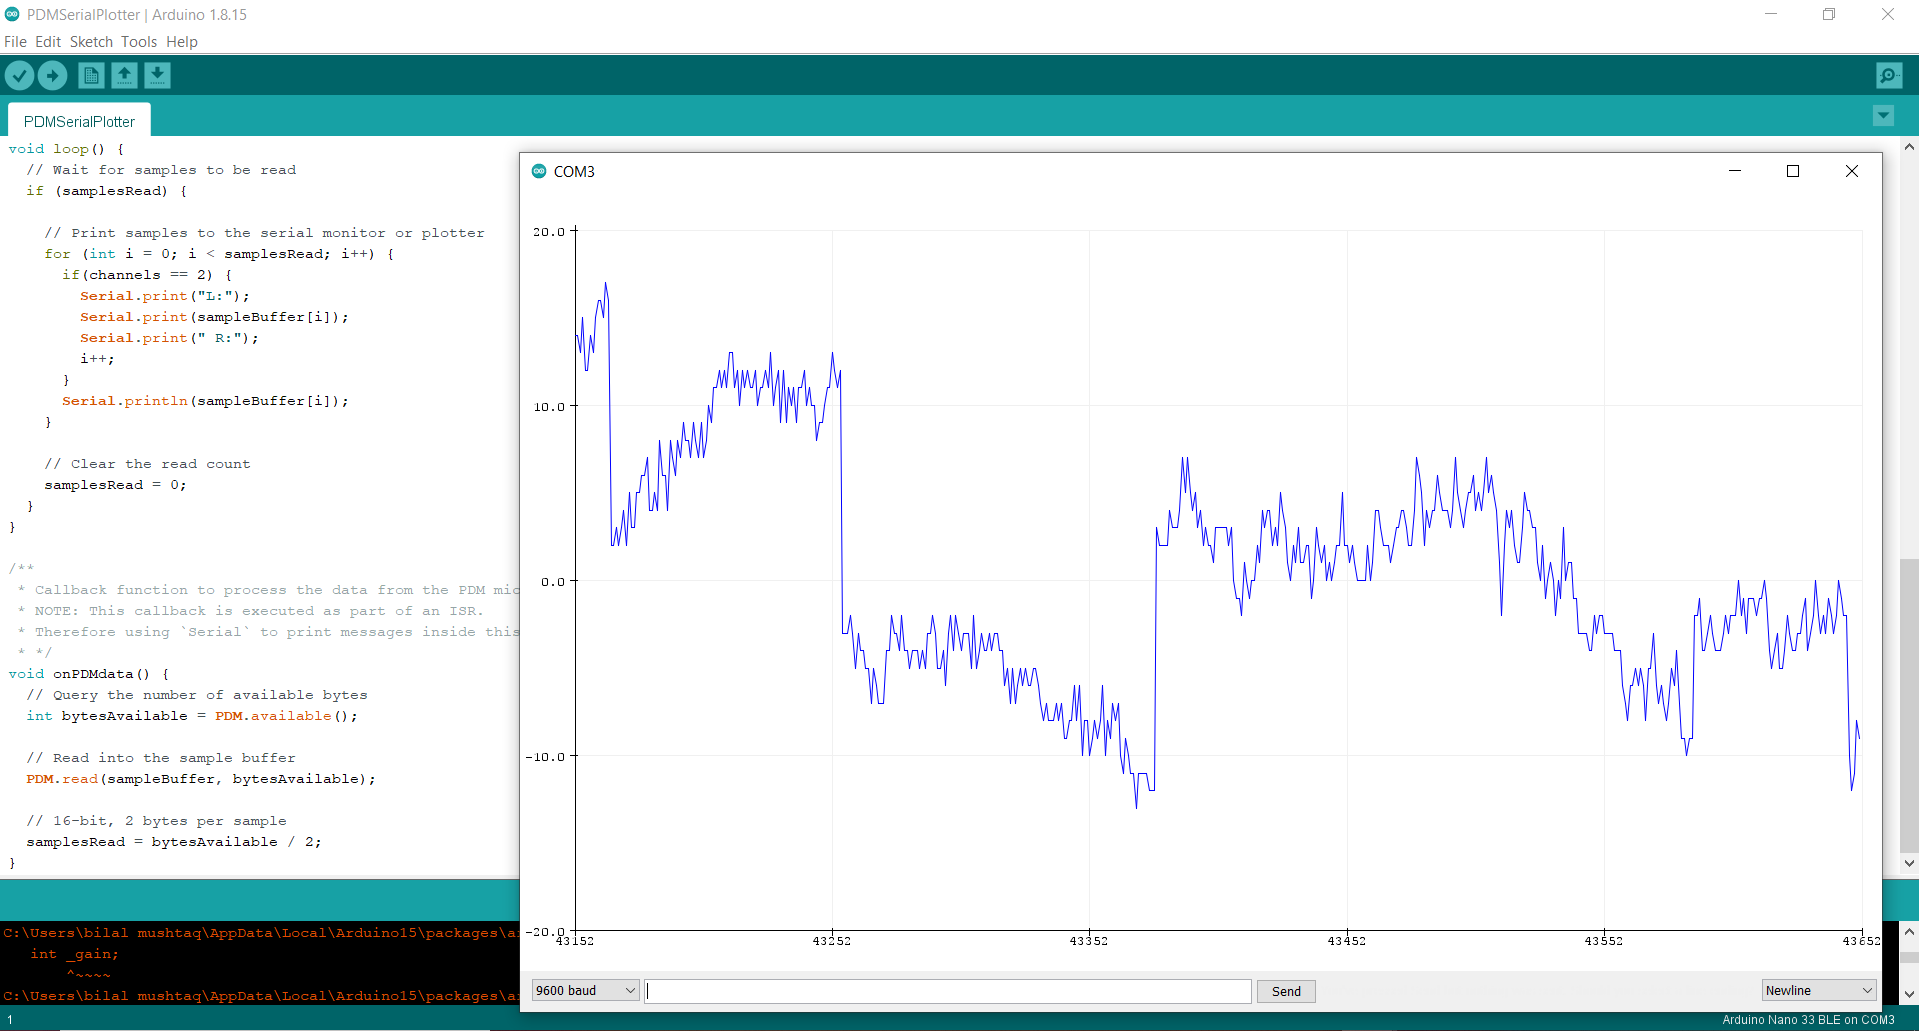
\includegraphics[width=8.5cm]{Nano33BLESense/10}
	\caption{MP34DT05, Serial Plotter}
	\label{fig:8}
\end{figure}

\section{Test with Bluetooth Module Connection}

The same procedure we need to follow for making the successful bleutooth coonection, the one we follow for on-board sensors. Below figure \ref{fig:testsoftware-fur-bluetooth} shows the ArduinoBLE library in the example section of Arduino IDE.



\begin{figure}[h]
	\centering
	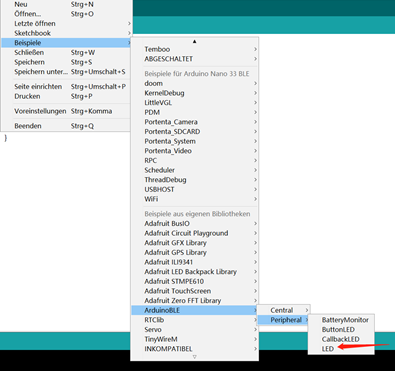
\includegraphics[width=0.7\linewidth]{Nano33BLESense/TestsoftwareBluetooth}
	\caption{Bluetooth Connection}
	\label{fig:testsoftware-fur-bluetooth}
\end{figure}

Bluetooth wireless technology allows us to share the data, the voice, the music, the video, and a lot of information between paired devices, It is built into many products, from mobile phones, cars to medical devices and computers. It has lower power consumption. It is easily upgradeable. It has range better than Infrared communication. Bluetooth is used for voice and data transfer, we can communicate by recieving and sending the data with other bluetooth connected devices. It is also possible to output a value on the phone side or also on the laptop by making the proper pairing. 


